%% -----------------------------------------------------------------------
%% -----------------------------------------------------------------------
%% Copyright 2024 by Bárbara Circe (barbara.circe@outlook.com)
%% **** Copyright notice: the following code is adapted from abnTeX2 package
%%									provided by Lauro César Araujo ****
%% -----------------------------------------------------------------------
%% This work may be distributed and/or modified under the
%% conditions of the LaTeX Project Public License, either version 1.3
%% of this license or (at your option) any later version.
%% 
%% Last Update: Janeiro 2024
% ------------------------------------------------------------------------
% ------------------------------------------------------------------------
% Modelo de Trabalho Acadêmico - Universidade Federal do Maranhão (UFMA)
% tese de doutorado, dissertação de mestrado e trabalhos monográficos 
% em geral em conformidade com ABNT NBR 14724:2011
% ------------------------------------------------------------------------
% ------------------------------------------------------------------------

\documentclass[
	% -- opções da classe memoir --
	12pt,				% tamanho da fonte
	openright,			% capítulos começam em pág ímpar (insere página vazia caso preciso)
	twoside,			% para impressão em recto e verso. Oposto a oneside
	a4paper,			% tamanho do papel. 
	% -- opções da classe abntex2 --
	chapter=TITLE,		% títulos de capítulos convertidos em letras maiúsculas
	%section=TITLE,		% títulos de seções convertidos em letras maiúsculas
	%subsection=TITLE,	% títulos de subseções convertidos em letras maiúsculas
	%subsubsection=TITLE,% títulos de subsubseções convertidos em letras maiúsculas
	% -- opções do pacote babel --
	english,			% idioma adicional para hifenização
	french,				% idioma adicional para hifenização
	spanish,			% idioma adicional para hifenização
	brazil				% o último idioma é o principal do documento
	]{abntex2}

% -----------------------------------
% Carregamento e configuração pacotes
% -----------------------------------
\usepackage{ufma-circe}
\citeoption{num}
\citebrackets{[}{]}
\usepackage{multirow}
% ---------------------------------------------------
% Informações de dados para CAPA e FOLHA DE ROSTO
% ---------------------------------------------------
\titulo{CLASSIFICAÇÃO DE ESPECTROS DE IMPEDÂNCIA POR INTELIGÊNCIA ARTIFICIAL}
\autor{JHERFSON CASTRO GOMES}
\local{São Luís - MA}
\data{2026}
\orientador{Prof. Dr. Clenilton Costa dos
Santos}
\coorientador{Prof. Dr. Rodolpho Mouta Monte Prado
}
\curso{CENTRO DE CIÊNCIAS EXATAS E TECNOLOGIA - CCET

CURSO DE FÍSICA - LICENCIATURA/CCET}
\instituicao{%
  Universidade Federal do Maranhão
  \par
  \imprimircurso
  \par
  Programa de Pós-Graduação}
\tipotrabalho{Monografia}		%Tese (Doutorado)}

% O preambulo deve conter o tipo do trabalho, o objetivo, 
% o nome da instituição e a área de concentração

\preambulo{Trabalho de Conclusão do Curso, como requisito obrigatório para a obtenção do título
de Licenciatura em Física pela da Universidade Federal do Maranhão (UFMA), Campus de São Luís, MA. }
% ---

% ----------------------------------------------------
% Configurações de aparência do PDF final
% ----------------------------------------------------
% alterando o aspecto da cor azul
\definecolor{blue}{RGB}{0,0,0}

% informações do PDF
\makeatletter
\hypersetup{
     	%pagebackref=true,
			pdftitle={\@title}, 
			pdfauthor={\@author},
    	pdfsubject={\imprimirpreambulo},
	    pdfcreator={LaTeX with abnTeX2},
			pdfkeywords={abnt}{latex}{abntex2}{trabalho acadêmico}{ufma}, 
			colorlinks=true,       													% false: boxed links; true: colored links
    	linkcolor=black,          												% color of internal links
    	citecolor=black,        													% color of links to bibliography
    	filecolor=magenta,      													% color of file links
			urlcolor=blue,
			bookmarksdepth=4
}
\makeatother

% ---
% compila o indice
% ---
\makeindex

% ---------------------------------------------------------
% Início do documento
% ---------------------------------------------------------
\begin{document}

%% Language 
%\selectlanguage{english}
\selectlanguage{brazil}

\frenchspacing 										% Retira espaço extra obsoleto entre as frases.

%!TEX root = ./main.tex
%%%%%%%%%%%%%%%%%%%%%%%%%%%%%%%%%%%%%%%%%%%%%%%%%%%%%%%%%%%%%%%%%%%%%%%%%%%%%%%%%%
% ----------------------------------------------------------
% ELEMENTOS PRÉ-TEXTUAIS
% ----------------------------------------------------------
% \pretextual

% ---
% Capa
% ---

\begingroup

\newgeometry{left=3cm,right=3cm,top=2cm,bottom=1.25cm}
\centering
\imprimircapa

% ---
% Folha de rosto
% (o * indica que haverá a ficha bibliográfica)
% ---

\imprimirfolhaderosto*

\endgroup

% ---
% Inserir a ficha bibliografica
% ---

% Isto é um exemplo de Ficha Catalográfica, ou ``Dados internacionais de
% catalogação-na-publicação''. Você pode utilizar este modelo como referência. 
% Porém, provavelmente a biblioteca da sua universidade lhe fornecerá um PDF
% com a ficha catalográfica definitiva após a defesa do trabalho. Quando estiver
% com o documento, salve-o como PDF no diretório do seu projeto e substitua todo
% o conteúdo de implementação deste arquivo pelo comando abaixo:
%
% \usepackage{pdfpages}		% necessário para comando \includepdf
% \begin{fichacatalografica}
%     \includepdf{fig_ficha_catalografica.pdf}
% \end{fichacatalografica}

% ficha catalográfica meio zoada mas funciona! :p
\begingroup
\newgeometry{left=3cm,right=3cm,top=2cm,bottom=2cm}
\centering
\begin{fichacatalografica}
	\sffamily
	\vspace*{\fill}					% Posição vertical
	\begin{center}				% Minipage Centralizado
	\framebox[130mm]{\indent\begin{minipage}[75mm]{125mm}		% Largura
	\smallskip
	\small
	\justifying{

	% \imprimirautor
	%Sobrenome, Nome do autor
	Castro Gomes, Jherfson  

 \imprimirtitulo  / \imprimirautor. -- \imprimirlocal, \imprimirdata- \\
	
 \thelastpage p. : il. (algumas color.) ; 30 cm. \\
	
 \imprimirorientadorRotulo~\imprimirorientador \par
 {\imprimirtipotrabalho~--~\imprimirinstituicao, \imprimirdata.} \\
	
		1. espectro de impedância.
		2. deep learning.
		2. machine learning. 
    I. Prof. Dr. Clenilton Costa dos Santos. 
    II. Universidade Federal do Maranhão.
		III. Física.
		IV. Título. 			}

	\smallskip
	\end{minipage}}
	\end{center}
\end{fichacatalografica}
\restoregeometry
\endgroup

% ---

% ---
% Inserir errata
% ---
% sem errata
% ---

% ---
% Inserir folha de aprovação
% ---

% Isto é um exemplo de Folha de aprovação, elemento obrigatório da NBR
% 14724/2011 (seção 4.2.1.3). Você pode utilizar este modelo até a aprovação
% do trabalho. Após isso, substitua todo o conteúdo deste arquivo por uma
% imagem da página assinada pela banca com o comando abaixo:
%
% \begin{folhadeaprovacao}
% \includepdf{folhadeaprovacao_final.pdf}
% \end{folhadeaprovacao}
%
\begingroup

\newgeometry{left=3cm,right=3cm,top=3cm,bottom=1.25cm}
\centering
\begin{folhadeaprovacao}

  \begin{center}
    {\ABNTEXchapterfont\normalfont\normalsize\MakeUppercase\imprimirautor}

    \vspace*{\fill}\vspace*{\fill}
    \begin{center}
      \ABNTEXchapterfont\bfseries\large\MakeUppercase\imprimirtitulo
    \end{center}
    \vspace*{\fill}
    
    \hspace{.45\textwidth}
    \begin{minipage}{.5\textwidth}
        \imprimirpreambulo
    \end{minipage}%

   \vspace*{\fill}
   \vfill     
   Trabalho aprovado. \imprimirlocal, -- de julho de 2026

   \end{center}

   \assinatura{\textbf{ Prof. Dr. Clenilton Costa dos Santos} (Orientador) \\ Universidade Federal do Maranhão - UFMA}   
   \assinatura{\textbf{ Prof. Dr. Rodolpho Mouta Monte Prado} (Coorientador) \\ Universidade Federal do Ceará - UFC}
    \assinatura{\textbf{Prof. Me. Micael Rocha de Azevêdo} 
    \\ Universidade Estadual do Sudoeste da Bahia - UESB}    
    \assinatura{\textbf{Profa. Dra. Carleane Patrícia da Silva Reis}
     \\Laboratório Ibérico Internacional de Nanotecnologia - INL}
   %\assinatura{\textbf{Professor} \\ Convidado 3}
   %\assinatura{\textbf{Professor} \\ Convidado 4}
      
   \begin{center}
    \vspace*{2.5cm}
    {\large\imprimirlocal}
    \par
    {\large\imprimirdata}
    \vspace*{1cm}
  \end{center}
  
\end{folhadeaprovacao}
\endgroup

% ---

% ---
% Dedicatória
% ---
% sem dedicatória
% ---

% ---
% Agradecimentos
% ---
\begin{agradecimentos}
Agradeço ao professo Rodolpho e ao professor Clenilton pela orientação, pela disponibilidade e pelo conhecimento compartilhado ao longo deste trabalho e do curso. A dedicação de vocês foi fundamental para que este projeto se tornasse realidade. 

À minha amiga Itxasne e a todos que estiveram presentes durante esses anos de cursos, pelas conversas, pelo apoio nos momentos difíceis, pelas risadas e por tornarem essa jornada muito mais leve. A companhia de vocês fez toda a diferença. 

À minha esposa, Iatamana, meu maior suporte. Obrigado pela paciência, pelo incentivo constante e por estar ao meu lado em cada etapa – especialmente nas mais difíceis. Sem você, nada disso faria sentido.  

À minha família, pelo amor incondicional e pela torcida de sempre. Vocês são a minha base. 

Agradeço à Fundação de Amparo à Pesquisa e ao Desenvolvimento Científico e Tecnológico do Maranhão (FAPEMA) e ao Conselho Nacional de Desenvolvimento Científico e Tecnológico (CNPq) pelo apoio concedido ao longo deste trabalho, por meio do incentivo à pesquisa científica.

Portanto, agradeço a todas as pessoas que de alguma forma passaram pela minha vida e deixaram algo. Cada encontro, cada conversa e cada experiência contribuiu para quem eu sou hoje e para chegar até aqui. 

\end{agradecimentos}
% ---

% ---
% Epígrafe
% ---
% sem epígrafe

% ---
% RESUMOS
% ---

% resumo em português
\setlength{\absparsep}{18pt} % ajusta o espaçamento dos parágrafos do resumo
\begin{resumo}
 O desenvolvimento de materiais para baterias recarregáveis tem despertado crescente interesse devido à expansão dos dispositivos de armazenamento de energia e à necessidade de tecnologias mais eficientes e sustentáveis. Nesse cenário, a Espectroscopia de Impedância (IS) constitui uma das principais técnicas para caracterizar eletrólitos sólidos para baterias recarregáveis, permitindo determinar propriedades como a condutividade iônica. No entanto, a interpretação dos espectros e a seleção do circuito equivalente mais adequado para o ajuste dos dados ainda dependem, em grande parte, da experiência do pesquisador, tornando esse processo demorado e sujeito a interpretações distintas. Diante desse desafio, este trabalho propõe a aplicação de técnicas de Inteligência Artificial (AI) para automatizar a classificação de espectros de impedância.
 Para o treinamento dos modelos, foi desenvolvido um banco de dados composto por espectros sintéticos gerados a partir de diferentes circuitos equivalentes e combinações de valores dos parâmetros doa elementos desses circuitos. Inicialmente, foram avaliados modelos baseados em \textit{Deep Learning} (DL), cujos resultados evidenciaram a importância da etapa de pré-processamento dos dados. Após a normalização dos espectros, observou-se um aumento significativo na precisão da classificação. Em seguida, foram implementados e comparados diferentes algoritmos de \textit{Machine Learning} (ML	), que apresentaram desempenho superior para o conjunto de dados estudado. A otimização dos hiperparâmetros também contribuiu para melhorar a capacidade de classificação dos modelos.
 Os resultados obtidos demonstram que técnicas de \textit{Machine Learning} constituem uma alternativa promissora para auxiliar na identificação automática do circuito equivalente associado aos espectros de impedância, reduzindo o tempo de análise e a subjetividade do processo. Como perspectivas futuras, destacam-se a incorporação de ruídos aos espectros sintéticos, a ampliação do banco de dados com diferentes faixas de frequência e a avaliação dos modelos utilizando dados experimentais. Espera-se que a metodologia proposta contribua para acelerar a caracterização de materiais e o desenvolvimento de novos eletrólitos sólidos e eletrodos para baterias recarregáveis, tornando o processo de pesquisa mais eficiente e confiável.

 \textbf{Palavras-chave}: Espectro de impedância. Deep learning. Machine Learning. 
\end{resumo}

% resumo em inglês
\begin{resumo}[Abstract]
 \begin{otherlanguage*}{english}
  The development of materials for rechargeable batteries has attracted increasing interest due to the rapid expansion of energy storage devices and the growing demand for more efficient and sustainable technologies. In this context, electrochemical impedance spectroscopy (EIS) has become one of the primary techniques for characterizing solid electrolytes and electrode materials, enabling the determination of properties such as ionic conductivity. However, the interpretation of impedance spectra and the selection of the most appropriate equivalent circuit for data fitting still rely heavily on the researcher's expertise, making the analysis time-consuming and subject to different interpretations. To address this challenge, this work proposes the application of artificial intelligence (AI) techniques to automate the classification of impedance spectra.  
  To train the models, a database consisting of synthetic spectra generated from different equivalent circuits and combinations of electrical parameters was developed. Initially, deep learning-based models were evaluated, and the results highlighted the importance of the data preprocessing stage. After spectrum normalization, a significant improvement in classification accuracy was observed. Subsequently, different machine learning (ML) algorithms were implemented and compared, demonstrating superior performance for the dataset investigated. Hyperparameter optimization further enhanced the classification capability of the models.  
  The results demonstrate that machine learning techniques provide a promising approach for assisting in the automatic identification of the equivalent circuit associated with impedance spectra, reducing both the analysis time and the subjectivity of the process. Future work includes incorporating noise into the synthetic spectra, expanding the database to cover different frequency ranges, and evaluating the models using experimental data. The proposed methodology is expected to accelerate the characterization of materials and the development of new solid electrolytes and electrode materials for rechargeable batteries, making the research process more efficient, reliable, and reproducible. 

   \vspace{\onelineskip}
 
   \noindent 
   \textbf{Keywords}: Impedance spectrum. Deep Learning. Machine Learning.
 \end{otherlanguage*}
\end{resumo}



\input{ListasSumario.tex}

% ----------------------------------------------------------
% ELEMENTOS TEXTUAIS
% ----------------------------------------------------------
\textual 													% início de elementos textuais, páginas com algarismos arábicos

%!TEX root = ./main.tex
%%%%%%%%%%%%%%%%%%%%%%%%%%%%%%%%%%%%%%%%%%%%%%%%%%%%%%%%%%%%%%%%%%%%%%%%%%%%%%%%%%
% ----------------------------------------------------------
% Introdução (exemplo de capítulo sem numeração, mas presente no Sumário)
% ----------------------------------------------------------
\chapter{Introdução}
Tem havido grande busca por fontes de energia limpa, devido à urgência climática
para que haja o abandono de uso dos combustíveis fósseis, e essa energia deve ser armazenada
em dispositivos como baterias recarregáveis de baixo custo e seguras. Pela mesma razão, o mercado
de veículos elétricos (EVs) tem crescido e recebido muitos investimentos. Em 2025, as vendas
de EVs corresponderam a aproximadamente 14\% de carros vendidos de todo o mundo \cite{IEA2026}. Para os EVs terem
uma maior utilização e aceitação no mercado, as baterias precisarão, entre outros fatores, ser
mais seguras \cite{olivetti2017lithium,armand2008building}. A segurança das baterias pode, em princípio, ser melhorada pela
substituição dos eletrólitos líquidos por eletrólitos sólidos ou pelo uso de revestimento dos
cátodos. Um dos requerimentos básicos tanto para eletrólitos quando para revestimento de cátodos
de baterias e íons de lítio (LIBs, do inglês \textit{lithium-ion batteries}) é ter condutividade iônica da ordem
de $1\,\mathrm{mS/cm}$. A determinação experimental dessa propriedade requer o ajuste de espectros de
impedância (IS, do inglês \textit{Impedance Spectroscopy}) usando um circuito equivalente como modelo \cite{sinfronio2018effect,santos2018chitosan}, que
consiste em componentes como resistores, capacitores, indutores e outros elementos.
Dependendo da qualidade do circuito e da experiência do pesquisador, pode se tornar uma
tarefa difícil identificar o modelo do circuito, além de consumo bastante tempo nessa
tarefa. Uma possível ferramenta que pode ser utilizada para identificar o modelo do circuito é a inteligência artificial \cite{zhu2019equivalent,huang2021towards,obregon2023convolutional,buteau2019analysis}. Portanto, neste trabalho, projetamos modelos
de inteligência artificial para identificar os modelos de circuitos equivalentes do espectro de
impedância equivalente.

\pagebreak

\chapter{Fundamentação Teórica}

\section{Espectroscopia de Impedância}

A espectroscopia de impedância (ES) é uma técnica utilizada para estudar, dentre outros sistemas, sólidos cerâmicos, monocristais
 em equilíbrio ou estado estacionário. Ela consiste na aplicação de um sinal senoidal (diferença de
potencial ou uma corrente alternada) em uma ampla faixa de frequências, perturbando o
sistema, e em seguida, monitorando a resposta senoidal do sistema em relação à perturbação
aplicada. Ademais, pode ser usada para analisar processos em interfaces eletrodo-eletrólito. 

Ao realizar a transição de um circuito em corrente continua (DC) para um circuito
em corrente alternada (AC), é necessário levar em conta que, além de os resistores (R) oferencerem resistência à passagem de corrente
os capacitores (C) e indutores (L) também são responsáveis por uma oposição à variação da corrente alternada, denominada reatância. 
A principal diferença entre resistência e reatância, em termos de dissipação de energia, é que a resistência está associada à dissipação de energia na forma de calor, 
enquanto a reatância está associada ao armazenamento periódico de energia em campos elétricos e magnéticos, sem perdas de calor.
A combinação de resistências e reatância é conhecida como impedância (Z) que é
calculada analisando a tensão em cada um dos componentes em série, como ilustrado na Figura~\ref{figura1}. Nessa análise, consideramos que a corrente que passa por eles segue a expressão $i = I \cos(\omega t)$, na qual $i$ representa o valor instantâneo da corrente em um determinado instante $t$.

As tensões instantâneas $v_{R}$, $v_{L}$ e $v_{C}$ em $R$, $L$ e $C$ são expressas, respectivamente,
por:
\begin{equation}
v_R = Ri = RI \cos(\omega t),
\label{eq:1}
\end{equation}
\begin{equation}
v_L = L\frac{di}{dt}
     = -\omega LI \sin(\omega t)
     = \omega LI \cos\left(\omega t + \frac{\pi}{2}\right),
     \label{eq:2}
\end{equation}
\begin{equation}
v_C = \frac{q}{C}
     = \frac{1}{\omega C}I \sin(\omega t)
     = \frac{1}{\omega C}I \cos\left(\omega t - \frac{\pi}{2}\right),
     \label{eq:3}
\end{equation}
%----imagem------
\begin{figure}[htbp]
    \centering
    \caption{Corrente $i$ fluindo através de $R$, $L$ e $C$ em série.}
    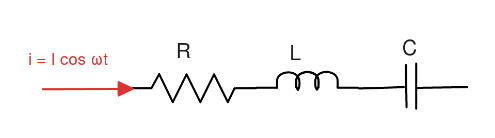
\includegraphics[width=0.6\textwidth]{Figuras/corrente_i.png}
    \legend{Fonte: Própria autoria.}
    \label{figura1}
\end{figure}
onde, na equação~\eqref{eq:3}, usamos a relação $q = \int i \, dt$. A equação~\eqref{eq:1} indica que o potencial $v_R$ está em fase com a corrente, enquanto $v_L$ está adiantada em $\frac{\pi}{2}$ em relação à corrente e $v_C$ está atrasada em $\frac{\pi}{2}$ em relação à corrente, podemos observar na Figura~\ref{figura2} as relações da corrente, tensão e fase.
\begin{figure}[htbp]
    \centering
    \caption{Diagrama de fasores (esquerda) e as formas de ondas sinusoidais correspondente à tensão $v(t)$ e à corrente $i(t)$, relações dos componentes: $(A)$
    resistor, $(B)$ capacitor e $(C)$ o indutor.}
    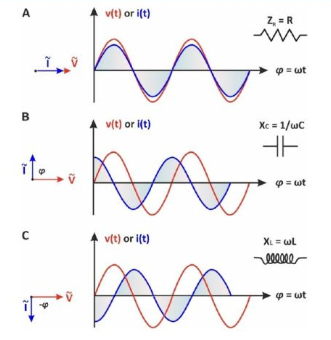
\includegraphics[width=0.5\textwidth]{Figuras/digrama_fasores.png}
    \legend{Fonte: Adaptado de \cite{lazanas2023electrochemical}.}
    \label{figura2}
\end{figure}

Os coeficientes $RI$, $\omega LI$ e $\left(\frac{1}{\omega C}\right)I$ têm unidade de volt e representam as amplitudes das tensões em $R$, $L$ e $C$, respectivamente. As Equações~\eqref{eq:1}, \eqref{eq:2} e \eqref{eq:3} indicam que, para uma frequência angular $\omega$ constante, existe uma relação de proporcionalidade entre as amplitudes da diferença de potencial e da corrente em cada elemento. Dessa forma, as Equações~\eqref{eq:2} e \eqref{eq:3} podem ser reescritas como:

\begin{equation}
    X_L = \omega L,
    \label{eq:4}
\end{equation}

\begin{equation}
    X_C = \frac{1}{\omega C},
    \label{eq:5}
\end{equation}
tanto $X_{L}$ quanto $X_{C}$ são expressões em ohm e medem a resistência oferecida pela indutância e pela capacitância, respectivamente, à corrente alternada em uma determinada frequência. A reatância indutiva é denominada por $X_{L}$, enquanto $X_{C}$ é chamada de reatância capacitiva. Podemos realizar a soma algébrica das três componentes $v_{R}$ + $v_{L}$ + $v_{C}$, portanto:
\begin{equation}
    v = RI\cos\omega t + \left(\frac{1}{\omega C} - \omega L\right) I \operatorname{sen} \omega t.
    \label{eq:6}
\end{equation}
Usando a relação trigonométrica do tipo $a \cos x + b \operatorname{sen} x$, ficando na forma $A\cos(x + \phi)$ e $\operatorname{tg}\phi = -\dfrac{b}{a}$, podemos reescrever a equação \eqref{eq:6} da seguinte forma:
\begin{equation}
    v = RI(\omega t + \phi) \rightarrow V\cos(\omega t + \phi).
    \label{eq:7}
\end{equation}
A amplitude da tensão pode ser escrita como
\begin{equation}
    V = \sqrt{(RI)^2 + \left[\left(\frac{1}{\omega C} - \omega L\right) I\right]^2},
    \label{eq:8}
\end{equation}
\begin{equation}
V = I\sqrt{R^2 + \left(\omega L - \frac{1}{\omega C}\right)^2} \rightarrow I\sqrt{R^2 + (X_L - X_C)^2}.
    \label{eq:9}
\end{equation}
O ângulo de defasagem entre a tensão e a corrente é dado por
\begin{equation}
    \phi = \operatorname{arctg}\frac{\omega L - \dfrac{1}{\omega C}}{R} \rightarrow \operatorname{arctg}\frac{X_L - X_C}{R}.
    \label{eq:10}
\end{equation}
O termo da radical na equação \eqref{eq:9}, geralmente é representado pela letra $Z$, é definido como a impedância dos elementos em série. Utilizando $Z$, podemos reescrever a equação:
\begin{equation}
    V = ZI.
    \label{eq:11}
\end{equation}
 Portanto, a equação é formalmente idêntica à lei de Ohm, na qual a impedância $Z$ desempenha o papel
equivalente à resistência em um circuito de corrente contínua.

\subsection{Resistor}
A corrente que atravessa um resistor é proporcional à tensão a que ele é submetido, de acordo com a seguinte equação:
\begin{equation}
    V = RI,
    \label{eq:12}
\end{equation}
sendo a constante de proporcionalidade $R$ na equação denominada resistência. Ao comparar a equação \eqref{eq:12} com a equação \eqref{eq:11}, podemos concluir que a impedância de um resistor é igual à resistência:
\begin{equation}
    Z_{R} = R.
    \label{eq:13}
\end{equation}
Considerando que a resistência é uma grandeza real, a impedância de um resistor é puramente real. Dessa forma, podemos representar o módulo da impedância da seguinte forma:
\begin{equation}
    |Z| = R.
    \label{eq:14}
\end{equation}
Sendo a parte real:
\begin{equation}
    Z' = R,
    \label{eq:15}
\end{equation}
e a parte imaginária:
\begin{equation}
    Z" = 0.
    \label{eq:16}
\end{equation}
Assim, com base na relação \eqref{eq:15}, podemos observar que a parte real da impedância permanece constante independentemente da frequência.
Em um circuito puramente resistivo, a impedância não possui uma parte imaginária, sendo representada apenas pela resistência do elemento. Assim, um resistor ideal é representado em um diagrama de Nyquist, além disso é representado por uma série de pontos sobrepostos na mesma posição, na qual cada ponto corresponde a uma frequência medida. Podemos ver essa representação na Figura~\ref{figura3}.
\begin{figure}[htbp]
    \centering
    \caption{Diagrama de Nyquist de um resistor.}
    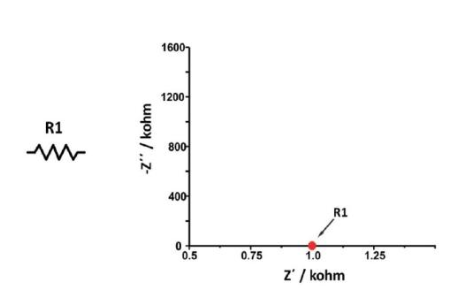
\includegraphics[width=0.8\textwidth]{Figuras/diagrama de Nyquist de um resistor..png}
    \legend{Fonte: Adaptado de \cite{lazanas2023electrochemical}.}
    \label{figura3}
\end{figure}

\subsection{Capacitor}
Uma corrente constante não pode fluir através de um capacitor, mas a carga elétrica pode se acumular nele, além disso, essa carga é diferente para cada tensão aplicada. Vimos a relação fundamental entre a carga e tensão na equação \eqref{eq:3} e, também, a reatância capacitiva na
expressão \eqref{eq:5}. Então, a impedância de um capacitor será descrita como:
\begin{equation}
    Z_C = \frac{i}{\omega C'},
    \label{eq:17}
\end{equation}
uma vez que a capacitância é uma grandeza real, a impedância de um capacitor é
puramente imaginária. Portanto, podemos expressar o módulo da impedância da seguinte forma:
\begin{equation}
    |Z| = \frac{1}{\omega C'}.
    \label{eq:18}
\end{equation}
Sendo a parte real:
\begin{equation}
    Z' = 0,
    \label{eq:19}
\end{equation}
e a parte imaginária:
\begin{equation}
    Z'' = \frac{1}{\omega C'}.
    \label{eq:20}
\end{equation}
Ao analisar as equações \eqref{eq:18}, \eqref{eq:19} e \eqref{eq:20}, é possível notar que a parte imaginária da impedância
apresenta um sinal oposto ao módulo da impedância. Além disso, é importante ressaltar que a
impedância de um capacitor não possui uma parte real, somente a parte imaginária. Da mesma
forma que o resistor, podemos representar no diagrama de Nyquist da contribuição do capacitor
na Figura~\ref{figura4}.
\begin{figure}[htbp]
    \centering
    \caption{Diagrama de Nyquist de um capacitor.}
    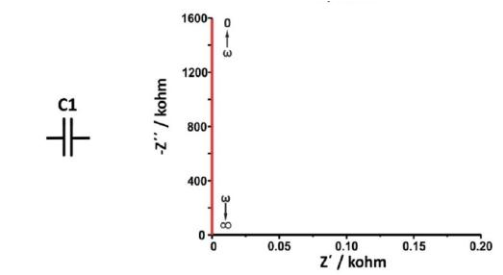
\includegraphics[width=0.8\textwidth]{Figuras/diagrama de Nyquist de um capacitor.png}
    \legend{Fonte: Adaptado de \cite{lazanas2023electrochemical}.}
    \label{figura4}
\end{figure}

\subsection{Indutor}
Quando uma corrente elétrica flui através de um indutor, ela gera um campo magnético ao seu redor. Esse campo magnético armazena energia e produz uma força que se
opõe a quaisquer alterações na corrente elétrica que o percorre. Além disso, observamos a relação fundamental
entre a carga e tensão na \eqref{eq:2}. Vimos também a reatância indutiva na expressão \eqref{eq:4} e,
dessa forma, podemos expressar a impedância de um indutor como:
\begin{equation}
    Z_{L}= i\omega L.
    \label{eq:21}
\end{equation}
A impedância de um indutor, assim como a impedância do capacitor, também é uma grandeza
puramente imaginária. Então, podemos escrever o módulo da impedância da seguinte forma:
\begin{equation}
    |Z| = \omega L.
    \label{eq:22}
\end{equation}
Sendo a parte real:
\begin{equation}
    Z' = 0,
    \label{eq:23}
\end{equation}
e a parte imaginária:
\begin{equation}
    Z" = \omega L.
    \label{eq:24}
\end{equation}
por meio das equações \eqref{eq:22}, \eqref{eq:23} e \eqref{eq:24}, observa-se que a parte imaginária da impedância corresponde
à impedância total do indutor. Na Figura~\ref{figura5}, temos o comportamento de um indutor representado
pelo diagrama de Nyquist.
\begin{figure}[htbp]
    \centering
    \caption{ Diagrama de Nyquist de um indutor ideal.}
    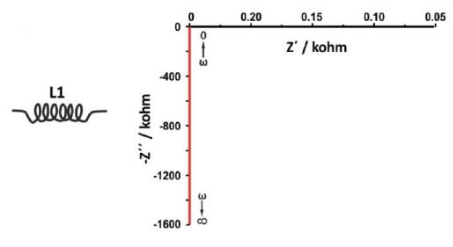
\includegraphics[width=0.8\textwidth]{Figuras/diagrama de Nyquist de um indutor ideal.png}
    \legend{Fonte: Adaptado de \cite{lazanas2023electrochemical}.}
    \label{figura5}
\end{figure}

\subsection{Impedância de Uma Associação de Elementos de Circuito}
Umas das grandes vantagens do EIS é a possibilidade de simular os dados em um
circuito elétrico equivalente e, dessa forma, obter valores numéricos para os componentes presentes no circuito. Para esse propósito, é possível utilizar o software fornecido junto aos analisadores de resposta em frequência ou software mais especializados, como o Zview \cite{dreher2005correlation} e outros existente no mercado. A qualidade da modelagem dos dados em relação a um circuito elétrico equivalente específico é avaliada pelo valor da distribuição \textit{chi-square} ($\chi^2$) \cite{lancaster2005chisquare}. No entanto, é importante destacar que não há um único modelo de circuito para um determinado espectro de impedância. Ademais, é possível simular um espectro de impedância com mais de um circuito, já que alguns circuitos podem ser matematicamente idênticas.

Para modelar as amostras, é usado a lei de Kirchoff, de modo que é calculado a
impedância em associações em série, indicada na equação \eqref{eq:25}, e em paralelo, indicada na equação \eqref{eq:26}, da seguinte forma:
\begin{equation}
Z = \sum_{i} Z_i = Z_1 + Z_2 + \cdots,
\label{eq:25}
\end{equation}

\begin{equation}
\frac{1}{Z} = \sum_{i} \frac{1}{Z_i}
= \frac{1}{Z_1} + \frac{1}{Z_2} + \cdots,
\label{eq:26}
\end{equation}
onde $Z{i}$ é a impedância do elemento $i$.
No caso de um circuito elétrico equivalente simples, temos o exemplo do circuito (RC) em paralelo (Figura~\ref{figura6}). Dessa forma, o inverso da impedância é dado por:
\begin{equation}
\frac{1}{Z}
=
\frac{1}{Z_R}
+
\frac{1}{Z_C}
=
\frac{1}{R}
+
\frac{1}{\frac{1}{\omega C}},
\label{eq:27}
\end{equation}
\begin{equation}
\frac{1}{Z}
=
\frac{1}{R}
+
\omega C
=
\frac{1+\omega C R}{R}.
\label{eq:28}
\end{equation}
Portanto, a impedância é expressa da seguinte forma: 
\begin{equation}
Z
=
\frac{R}{1+i\omega RC}
=
\frac{R}{R^{2}C^{2}\omega^{2}+1}
-
i\,\frac{CR^{2}\omega}{R^{2}C^{2}\omega^{2}+1}.
\label{eq:29}
\end{equation}

\begin{figure}[htbp]
    \centering
    \caption{Representação de circuito RC paralelo.}
    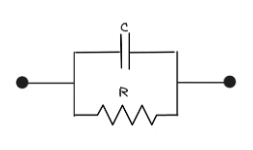
\includegraphics[width=0.5\textwidth]{Figuras/representação de circuito RC paralelo.png}
    \legend{Fonte: Própria autoria.}
    \label{figura6}
\end{figure}
Podemos substituir o $RC$ pelo $\tau$, que seria a constante de tempo de um processo ou o tempo de relaxamento \cite{lazanas2023electrochemical}. O circuito $RC$ pode ser representado usando o diagrama de Nyquist e é ilustrado como um semicírculo, na qual sob frequências muito altas a reatância capacitiva tente a zero
($\omega$ → $\infty$, $X_{c}$ → 0), resultando em toda a corrente fluindo pelo capacitor. Assim, o circuito se comporta
como um curto-circuito, e a impedância é zero. Por outro lado, em frequência muito baixas, a
reatância capacitiva tende ao infinito ($\omega$ → 0, $X_{c}$ → $\infty$), fazendo com que toda a corrente passe
pelo resistor. A impedância consiste apenas na parte real, $Z^{'}$ = $R1$.

Em resposta à discussão
anterior, quando $\omega$ → 0, a corrente se mantém constante. Essa corrente constante não pode
passar pelo capacitor, ela flui somente pelo resistor. Em frequência intermediárias, a corrente
passa simultaneamente pelo capacitor e pelo resistor, sendo a proporção das correntes
determinada pela oposição ao fluxo de corrente em cada ramo.
Ao transitar de frequências altas
para médias, a reatância capacitiva aumenta, porém ainda permanece menor que a resistência
ôhmica ($X_{c}$ < $R1$), o que resulta em uma maior passagem de corrente alternada pelo capacitor, enquanto menos corrente constante flui pelo resistor, como mostra na Figura ~\ref{figura7}.

No entanto, existe uma única frequência característica em que a reatância e a resistência possuem valores iguais ($X_c = R_1$). Nessa frequência, a parte imaginária da impedância ($Z''$) atinge seu valor máximo. Chamamos essa frequência angular de $\omega_{Z''\_max}$.
Como nessa frequência específica $\omega = \omega_{Z''\_max}$, substituímos na equação \eqref{eq:5}:

\begin{equation}
	R_1 = \frac{1}{\omega_{Z''\_max} \, C}.
	\label{eq:zma}
\end{equation}
Isolando $\omega_{Z''\_max}$,

\begin{equation}
	\omega_{Z''\_max} = \frac{1}{R_1 C}.
	\label{eq:30}
\end{equation}
Essa expressão pode ainda ser escrita em termos da constante de tempo $\tau = R_1 C_1$:

\begin{equation}
	\omega_{Z''\_max} = \frac{1}{R_1 C_1}= \frac{1}{\tau} .
	\label{eq:r1c1}
\end{equation}

Portanto, a constante de tempo característica do sistema, é representada por $\tau$ = $R_{1}C_{1}$, é determinada quando a parte imaginária e a parte real da impedância se igualam.

Um capacitor com um dielétrico imperfeito é melhor representado por um circuito RC em paralelo. Isso ocorre porque o dielétrico imperfeito causa uma perda de energia, o que faz com que o desfasamento entre a tensão aplicada e a corrente não seja exatamente de $90^\circ$. Nesse caso, os circuitos RC em paralelo são substituídos por um elemento de fase constante
(CPE), que são capazes de representar capacitores imperfeitos \cite{santos2018chitosan}, da seguinte forma:
\begin{equation}
Z_{\mathrm{CPE}}=\frac{1}{T(i\omega)^p},
\label{eq:31}
\end{equation}
na qual $\omega$ = 2$\pi f$ é a frequência angular em $rad/s$, sendo $p$ um parâmetro que varia de 0 à 1 que
descreve o deslocamento de fase e $T$ como pseudocapacitância $\mathrm{F}\cdot\frac{\mathrm{s}^{p-1}}{\mathrm{rad}^{p-1}}$. Quando temos
o resistor e o CPE em paralelo, pode ser nomeado como circuito RQ, podendo ser representada na equação \eqref{eq:32} e na Figura ~\ref{figura8}:
\begin{equation}
Z_{R\text{-}\mathrm{CPE}}
=
\frac{R}{1+\left(i\omega\tau\right)^p}.
\label{eq:32}
\end{equation}
\begin{figure}[htbp]
    \centering
    \caption{Representação do diagrama de Nyquist do circuito RC.}
    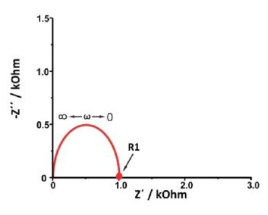
\includegraphics[width=0.5\textwidth]{Figuras/a representação do diagrama de Nyquist do circuito RC.png}
    \legend{Fonte: Adaptado de \cite{lazanas2023electrochemical}.}
    \label{figura7}
\end{figure}
\begin{figure}[htbp]
    \centering
    \caption{Representação do circuito RC.}
    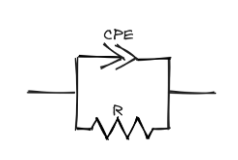
\includegraphics[width=0.3\textwidth]{Figuras/representação do circuito RQ.png}
    \legend{Fonte: Própria autoria.}
    \label{figura8}
\end{figure}

Dessa forma, podemos incluir mais componentes na simulação da modelagem dos
circuitos equivalentes e, consequentemente, aumentar sua complexidade ao identificar os
componentes.

\section{Aprendizado de Máquina (\textit{Machine Learning})}
Aprendizado de máquina (AM) é um ramo da inteligência artificial que se destaca por
sua capacidade de automatizar tarefas complexas através da análise de dados. Por meio de
algoritmos matemáticos e estatísticos, os computadores aprendem a identificar padrões e tomar
decisões sem serem explicitamente programados. Embora seus primórdios remontem a décadas
de 60, AM avançou nas últimas décadas impulsionado pelo avanço tecnológico. Inicialmente
restrito a aplicações computacionais, o AM expandiu-se para o campo interdisciplinar com
aplicações em diversas áreas, como medicina, economia, pesquisa cientifica, indústria,
marketing, detecção de fraudes, veículos autônomos e muitas outras aplicações \cite{geron2017handson}.

Os algoritmos de AM podem ser divididos em tipos de aprendizado de acordo com a
quantidade e o tipo de supervisão, sendo, aprendizado supervisionado e não supervisionado. Alguns autores, também consideram outros algoritmos, como o semi-
supervisionado e aprendizado por reforço\cite{geron2017handson,ludermir2021inteligencia}, conforme podemos ver na Figura~\ref{figura9}.
\begin{figure}[htbp]
    \centering
    \caption{Diagrama com os tipos de aprendizado em \textit{Machine Learning}.}
    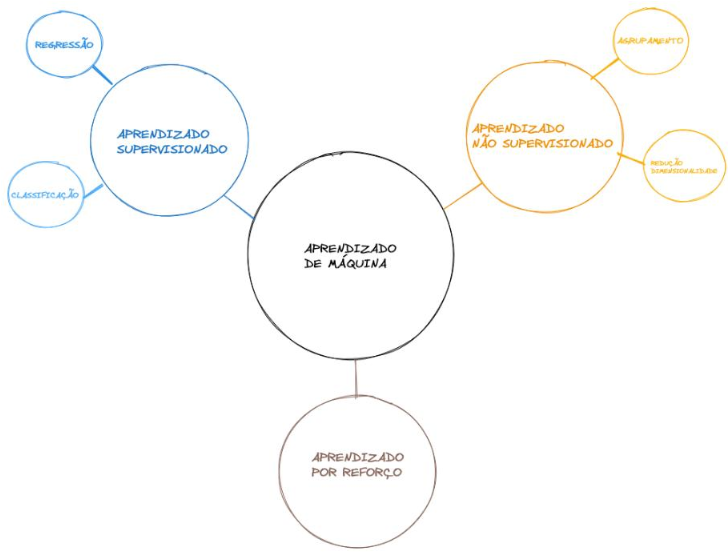
\includegraphics[width=0.8\textwidth]{Figuras/diagrama dos tipos de aprendizado em machine learning.png}
    \legend{Fonte: Própria autoria.}
    \label{figura9}
\end{figure}

No aprendizado supervisionando é fornecido conjuntos de dados com suas respectivas
saídas para o modelo, no caso, o modelo irá aprender com o problema e a solução fornecida.
Existem dois tipos de aprendizado supervisionado: a regressão, que é um método que utiliza
técnica estatística para modelar relações entre variáveis dependentes e independentes. E a
classificação, que é utilizado neste trabalho, e que será abordado com mais detalhes
posteriormente.
No aprendizado não supervisionado é treinando sem nenhum dado rotulado ou
categorias pré-definidas. Esse tipo de modelo identifica padrões, estruturas ou relações
referentes aos dados. Os principais algoritmos de aprendizado não supervisionado são:
agrupamento (clusterização), visualização e redução de dimensionalidade, detecção de
anomalias e de novidades, aprendizado de regras por associação ~\cite{geron2017handson, kubat2017introduction, goodfellow2016deep}.

\subsection{Classificação}
Conforme mencionado no subtópico anterior, a classificação é uma subcategoria do
aprendizado supervisionado, onde o algoritmo é treinado com um conjunto de dados que
contém rótulos ou classes associadas aos dados. O objetivo deste treinamento é preparar o
modelo para prever a classe ou categoria à qual os dados pertencem, com base nos padrões identificados nos dados de treinamento. Na classificação, o programa é solicitado a especificar
a qual das $k$ categorias uma entrada pertence. Para resolver essa tarefa, o algoritmo de
aprendizado é geralmente solicitado a produzir uma função $f$:$\mathbb{R}^{n}\rightarrow\{1,\ldots,k\}$. Quando $y$ = $f(x)$ o modelo associa uma entrada, descrita pelo vetor $x$, a uma categoria identificada por um
código numérico $y$ \cite{geron2017handson,kubat2017introduction,goodfellow2016deep}.

A classificação é uma técnica amplamente utilizada em diversas aplicações, tais como:
classificação de e-mail como spam, diagnóstico médico, reconhecimento de padrões de
imagens, como identificação de objetos, detecção de fraudes em transações financeiras e análise
de sentimento em processamento de linguagem natural. No campo da classificação, existem
diversos algoritmos, cada um com suas características distintas. Neste trabalho, foram
utilizados os seguintes algoritmos: \textit{Random Forest} (floresta aleatória), \textit{k-nearest neighbors} (k vizinhos mais próximos ou KNN), \textit{Decision Tree} (árvore de decisão), \textit{Logistic Regression}, \textit{Gaussian Naive Bayes}, \textit{Linear Support Vector Machine} (SVM), \textit{Extreme Gradient Boosting} (XGBoost), \textit{Gradient Boosting}, \textit{Stochastic Gradient Descent} e \textit{Light Gradient Boosting} (LightGBM).

O processo de treinamento de um modelo de classificação envolve várias etapas
necessárias. Primeiramente, ocorre a preparação do conjunto de dados de treinamento, no qual
o modelo recebe exemplos, cada um com atributos e uma classe ou categoria conhecida. Esses
exemplos são cruciais para que o modelo aprenda as relações entre os atributos e as classes.
Após isso, é selecionado um modelo de classificação mais adequado para o conjunto de dados.
O modelo, durante o treinamento, aprende os padrões nos dados e constrói uma função ou
mapeamento que relaciona as características de entrada (atributos) às classes. 

Posteriormente,
o modelo treinado se torna capaz de fazer previsões ou classificar novos exemplos. Para isso,
ele analisa as características dos novos exemplos e atribui uma classe com base no
conhecimento adquirido durante o treinamento. Por fim, a etapa final é avaliação do
desempenho do modelo. 

A qualidade de um modelo de classificação é medida por meio de
métricas como precisão, recall, f1-score, matriz de confusão e entre outras. Essa métricas
desempenham um papel fundamental ao determinar quão bem o modelo realiza suas previsões.
Além de todos esses processos, também precisamos avaliar se o modelo está sofrendo de
underfitting (subajuste), o que ocorre quando ele não é capaz de aprender todos os padrões e
informações relevantes nos dados de treinamento, ou overfitting, que é quando o modelo não
apenas aprende os padrões nos dados, mas também incorpora os ruídos e variações específicas
presentes nos dados de treinamento.
\subsubsection{Árvore de decisão (\textit{Decision Tree})}
A árvore de decisão é uma técnica de aprendizado supervisionado que se aplica a
problemas de classificação e regressão, mas é principalmente usada para resolver problemas de
classificação. O modelo age como um classificador em forma de árvore, onde os nós internos
representam os atributos de um conjunto de dados, os ramos denotam as regras de decisão e as
folhas contêm os resultados. A árvore de decisão apresenta dois tipos de nós de decisão e os
nós folha. Os nós de decisão desempenham um papel na tomada de decisão e se ramificam em
múltiplas direções, enquanto os nós folham representam as saídas dessas decisões sem novos
ramos. As decisões ou testes são realizados com base nos atributos do conjunto de dados
fornecido.

Essa técnica é uma representação gráfica que visa encontrar todas as soluções
possíveis para um problema ou decisão, com base em condições predefinidas. Podemos ver um
exemplo de como a árvore de decisão funciona, utilizando o conjunto de dados de íris. 

O termo árvore de decisão se justifica pelo fato de ela começar com um nó raiz, semelhante ao tronco
de uma árvore, que se ramifica em outros nós e cria uma estrutura semelhante a galhos de
árvore. 

Para construir uma árvore de decisão, utilizamos o algoritmo CART, que significa
algoritmo de árvore de classificação e regressão. Na Figura~\ref{figura10}, temos uma predição usando o
conjunto de dados de íris \cite{fisher1936iris}. A classificação das flores
de íris inicia-se no nó raiz, situado na profundidade 0, no topo da árvore de decisão. Neste nó,
a primeira pergunta feita é: o comprimento da pétala da flor é inferior a 2.45 cm? Se a resposta
for afirmativa, prosseguimos para o nó filho esquerdo na profundidade 1. Este nó é
uma folha, o que significa que não há mais perguntas a serem feitas. A árvore de decisão prevê
que a flor é uma íris setosa. Por outro lado, se o comprimento da pétala for superior a 2.45 cm,
descemos para nó filho direito da raiz, também na profundidade 1, à direita. Este não é um nó
folha, portanto, ele faz uma nova pergunta: a largura da pétala é inferior a 1.75 cm? Se a
resposta for afirmativa, é provável que a flor seja uma íris versicolor profundidade 2, à esquerda.
Se a resposta for negativa, é provável que seja uma íris virginica profundidade 2, à direita \cite{geron2017handson}.

\begin{figure}[htbp]
    \centering
    \caption{Árvore de decisão do conjunto de dados da íris.}
    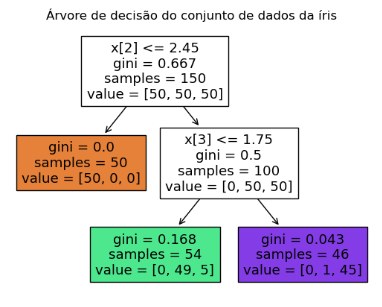
\includegraphics[width=0.5\textwidth]{Figuras/arvore de decisão do conjunto de dados da íris..png}
    \legend{Fonte: Própria autoria.}
    \label{figura10}
\end{figure}

As árvores de decisão oferecem várias vantagens. Elas são simples de entender e
visualizar, o que facilita a interpretação das decisões. Além disso, exigem menos preparação
dos dados em comparação com outras técnicas, o que significa menos trabalho com
normalização de dados e criação de variáveis \textit{dummy} (variáveis binárias). Outra vantagem é a
capacidade de lidar com diferentes tipos de dados, tanto numéricos quanto categóricos. Isso as
torna úteis em problemas com várias categorias.

Além disso, as árvores de decisão são
explicáveis, o que significa que você pode entender facilmente por que uma decisão foi tomada.
Elas também podem ser validadas usando testes estatísticos, o que ajuda avaliar o quão
confiável é o modelo. Mesmo quando algumas suposições são ligeiramente violadas pelo
modelo real que gerou os dados, as árvores de decisão geralmente mantêm um bom
desempenho.

No entanto, existem desvantagens a serem consideradas. As árvores de decisão
podem se tornar excessivamente complexas e se ajustar demais aos dados, um problema
conhecido como overfitting. Para evitar isso, são necessários mecanismos como poda ou a
limitação da profundidade máxima da árvore. Elas também podem ser instáveis, gerando
árvores completamente diferentes com pequenas variações nos dados.

O uso de conjuntos de
árvores (ensembles) ajuda a resolver esse problema. A aprendizagem de uma árvore de decisão
ideal é um problema complexo, e os algoritmos usam heurísticas, o que significa que não podem
garantir uma solução globalmente ideal. Além disso, algumas questões, como o problema XOR,
são difíceis de aprender com árvores de decisão. Por fim, as árvores de decisão podem criar árvores tendenciosas se algumas classes dominarem. Portanto, é aconselhável equilibrar o
conjunto de dados antes de ajustar a árvore de decisão.

Dados um conjunto de vetores de treinamento $x_i \in \mathbb{R}^n$, onde $i = 1, \ldots, l$ é um vetor de rótulos $y \in \mathbb{R}^l$, uma árvore de decisão particiona de forma recursiva o espaço de características para agrupar amostras com rótulos semelhantes em conjunto.  Cada nó $m$ contém um conjunto $Q_m$ de $n_m = Q_ml$ amostras de treinamento. Cada divisão candidata é representada por $\theta=(j,t_m)$, em que $j$ identifica um atributo e $t_m$ é o limiar aplicado a esse atributo. A divisão separa as amostras dois subconjuntos:   

\begin{equation}
    Q_m^{esquerda}(\theta) = \{(x,y) \mid x_j \leq t_m\},
    \label{eq:33}
\end{equation}

\begin{equation}
    Q_m^{direita}(\theta) = Q_m \setminus Q_m^{esquerda}(\theta).
    \label{eq:34}
\end{equation}

A qualidade de cada divisão candidata é avaliada pela impureza ponderada dos dois nós filhos, calculada por uma função $H$, como o índice de Gini ou a entropia. A melhor divisão é aquela que minimiza essa impureza pnderada ou, equivalentemente, maximiza a redução de impureza. A escolha da função depende da tarefa em questão, que pode ser classificação ou regressão. A métrica de qualidade $G(Q_m, \theta)$ é definida como:

\begin{equation}
    G(Q_m, \theta) = \frac{n_m^{esquerda}}{n_m} H\left(Q_m^{esquerda}(\theta)\right) + \frac{n_m^{direita}}{n_m} H\left(Q_m^{direita}(\theta)\right).
    \label{eq:35}
\end{equation}
O objetivo é selecionar os parâmetros que minimizam a impureza, logo

\begin{equation}
    \theta^* = \operatorname*{argmin}_{\theta} G(Q_m, \theta).
    \label{eq:36}
\end{equation}
Esse processo é repetido para os subconjuntos $Q_m^{esquerda}(\theta^*)$ e a $Q_m^{direita}(\theta^*)$ até que a profundidade máxima permitida seja alcançada, $n_m < min_{amostras}$ ou $n_m = 1$.

Considere um problema de classificação com $K$ classes, identificadas por $k=0, 1, ..., K-1$. Para cada nó $m$, a proporção de amostras pertencentes à classe $k$ é dada por:

\begin{equation}
    p_{mk} = \frac{1}{n_m} \sum_{y \in Q_m} I(y = k)
    \label{eq:37}
\end{equation}
em que $l(y_i = k)$ vale 1 quando a amostra $i$ pertence à classe $k$ e $O$ caso contrário. Se $m$ for um nó terminal essas proporções constituem as probabilidades estimadas retornadas pelo método $predict_proba$. A classe prevista é aquela que apresenta o maior valor de $p_mk$. As medidas comuns de impureza são as respectivamente Gini, dada pela equação \eqref{eq:38}, e Entropia, equação \eqref{eq:39}:
\begin{equation}
    H(Q_m) = \sum_{k} p_{mk}(1 - p_{mk}),
    \label{eq:38}
\end{equation}

\begin{equation}
    H(Q_m) = \sum_{k} p_{mk} \log(p_{mk}).
    \label{eq:39}
\end{equation}
Vale ressaltar que o conceito de entropia se originou como uma grandeza termodinâmica, entropia é uma medida estatística da multiplicidade de microestados, ou seja, a contagem de todas as maneiras pelas quais as partes um sistema podem se organizar para produzir o mesmo macroestado.
\subsubsection{\textit{Ensemble learning}}
\textit{Ensemble learning} ou (aprendizagem conjunto) é um método que consiste em combinar
as previsões de vários modelos individuais para poder generaliza-los e chegar em um modelo
finais mais preciso, como podemos ver na Figura~\ref{figura11}. No ensemble existe duas técnicas: o
\textit{bagging} e o \textit{boosting}.
\begin{figure}[htbp]
    \centering
    \caption{Representação dos modelos de ensemble.}
    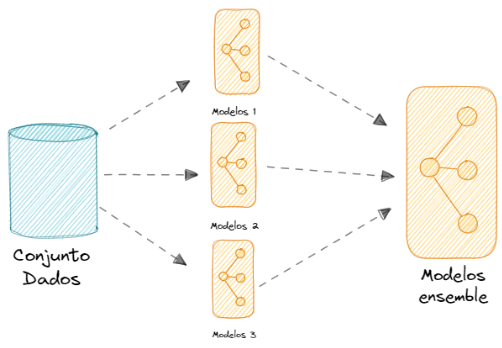
\includegraphics[width=0.5\textwidth]{Figuras/representação do ensemble.png}
    \legend{Fonte: Própria autoria.}
    \label{figura11}
\end{figure}
\subsubsection{\textit{Bagging}}
\textit{Bagging (Bootstrap aggregating)} é um método que utiliza um conjunto de dados de
amostragem aleatório como reposição, conhecido como \textit{bootstrap}, que é uma técnica estatística
amplamente utilizada \cite{efron1979bootstrap,breiman1996bagging}. Essa abordagem permite que os mesmos dados apareçam em vários subconjuntos, promovendo a robustez do modelo. 

No \textit{bagging}, os modelos de forma
individual em diferentes subconjuntos de dado, cada um aprendendo padrões específicos
encontrados em sua amostra, sem serem influenciados pelos outros modelos, Figura~\ref{figura12}. 

Essa
diversidade no treinamento dos modelos ajuda a reduzir a variância das previsões e evita
\textit{overfitting}, ou seja, o modelo se ajusta demais aos dados de treinamento e não generaliza bem
para novos dados. Assim, cada modelo preditivo explorará diferentes aspectos dos dados,
aumentando a robustez do conjunto.
\begin{figure}[htbp]
    \centering
    \caption{Representação da técnica \textit{bagging}, na qual são criados submodelos e, em seguida, são realizadas as predições.}
    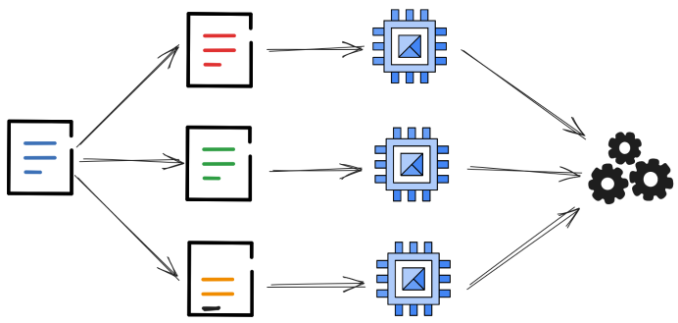
\includegraphics[width=0.8\textwidth]{Figuras/representação da técnica bagging. São criados submodelos em seguidos são realizadas prediçõe.png}
    \legend{Fonte: Própria autoria.}
    \label{figura12}
\end{figure}

Para regressão, as previsões dos modelos individuais são combinadas por meio da
média, enquanto para classificação, a combinação é feita por votação, onde a classe mais
frequente é selecionada como a previsão final. Essa abordagem resulta em previsões mais
estáveis e precisas, aproveitando as diferentes perspectivas fornecidas pelos modelos
individuais. 

No contexto deste trabalho, o algoritmo de \textit{bagging} utilizado foi o \textit{RandomForest},
que é um conjunto de árvores de dados. O \textit{RandomForest} combina os princípios do \textit{bagging}
com a construção de árvores de decisão, resultando em um modelo poderoso e versátil, capaz
de lidar com uma variedade de problemas de regressão e classificação.

\subsubsection{Floresta aleatória (\textit{Random Forest}, RF)}
\textit{Random forest} (RF) é um algoritmo de aprendizado de máquina supervisionado
utilizado tanto para problemas de regressão quanto para problemas de classificação. Além disso,
é conhecido por sua facilidade de uso e flexibilidade. Uma floresta é composta por várias árvores, sendo que quanto mais árvores compõem a floresta, mas robusta o modelo se torna. A
RF cria árvores de decisão selecionando aleatoriamente amostras de dados, obtendo previsões
para cada árvore e selecionando a melhor solução por votação.Além disso, fornece um bom
indicador da importância das características \cite{ho1995random}. 

As árvores de decisão individuais são geradas
usando indicadores de seleção de atributos, como ganho de informação, taxa de ganho e índice
Gini, como vimos na equação \eqref{eq:38}, e ou Entropia na equação \eqref{eq:39}, para cada atributo. Cada
árvore é construída com base em uma amostra aleatória independente dos dados. Em um
problema de classificação, cada árvore emite um voto e a classe mais popular é escolhida como
resultado final, como podemos ver na Figura~\ref{figura13}.
\begin{figure}[htbp]
    \centering
    \caption{Diagrama da estrutura do modelo RF.}
    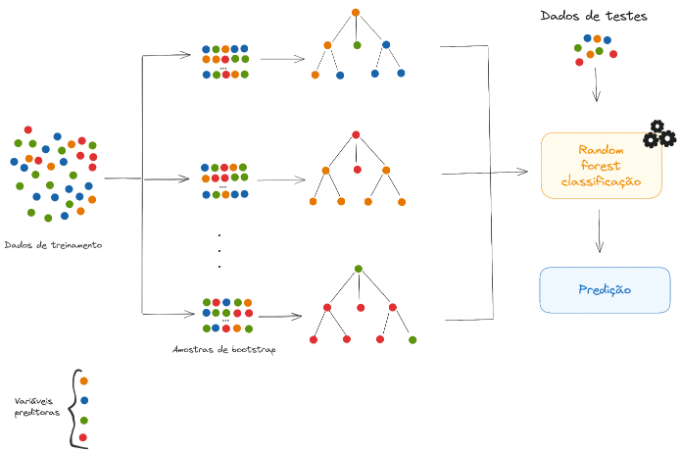
\includegraphics[width=0.8\textwidth]{Figuras/diagrama da estrutura do modelo RF.png}
    \legend{Fonte: Própria autoria.}
    \label{figura13}
\end{figure}

De forma semelhante ao método \textit{bagging}, a estrutura de funcionamento do algoritmo Floresta aleatória (\textit{Random Forest}, RF) consiste nas seguintes etapas:

• Seleciona-se aleatoriamente uma amostra de um conjunto de dados;

• Constrói-se uma árvore de decisão para cada amostra e obtém-se a previsão de cada árvore;

• Realiza-se uma votação para cada resultado previsto;

• Seleciona-se o resultado da previsão mais votado como o resultado final.

Ademais, árvore de decisão profundas podem
sofrer de \textit{overfitting}, mas RF previnem isso criando árvores em subamostras. Embora as árvores de decisão sejam computacionalmente rápidas, a RF é difícil de interpretar, são modelos que
são consideradas caixas pretas. Suas vantagens incluem alta precisão e robustez devido ao
grande número de árvores no processo, bem como a capacidade de lidar com valores ausente e
computar a importância das características.
\subsubsection{\textit{Boosting}}
É uma técnica de aprendizado em conjunto na qual vários modelos somples são treinados sequencialmente. Diferente do bagging, os modelos não são independentes: cada novo aprendiz é construído para reduzir os erros do conjunto formado pelos aprendizes anteriores. No AdaBoost, isso é feito aumentando  a importância das amostras classificadas incorrentamente. Em métodos de gradient boosting, como Gradient Boosting, XGBoost e LightGBM, cada novo modelo é treinado para aproximar uma direção de correção associada ao grandiente da função de perda. A previsão final resulta da combinação ponderada ou aditiva de todos os modelos treinados. A
Figura~\ref{figura14} ilustra o processo geral do Boosting, existem várias alternativas para determinar os
pesos a serem utilizados na próxima etapa. Essa técnica pode resultar em um modelo combinado
com menos erros, pois otimiza as vantagens e reduz as limitações no modelo único.
\begin{figure}[htbp]
    \centering
    \caption{Estrutura do Boosting}
    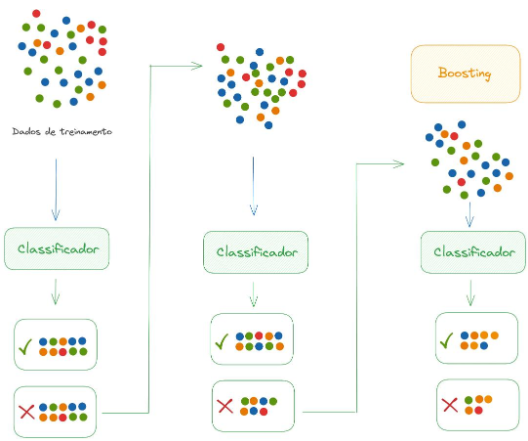
\includegraphics[width=0.8\textwidth]{Figuras/estrutura do Boosting.png}
    \legend{Fonte: Própria autoria.}
    \label{figura14}
\end{figure}

Nesse trabalho utilizamos alguns modelos de \textit{boosting}, incluindo \textit{gradient boosting},
\textit{Light Gradiente Boosting} e \textit{extreme gradiente boosting}. Vamos examinar cada um com mais
detalhes.
\subsubsection{\textit{Gradient Boosting}}
O \textit{Gradiente boosting} (GB) é um algoritmo de \textit{boosting} que pode ser usado tanto para
regressão quanto para classificação. Esse método utiliza uma técnica de ensemble que combina
os resultados de preditores fracos, onde cada um tem o objetivo de minimizar o erro do modelo
anterior por meio de uma função de perda diferenciável arbitrária.

Embora geralmente sejam
usadas árvores de decisão como modelo fracos, isso não é uma regra. Cada ajuste dos modelos
fracos é multiplicado por um valor chamado taxa de aprendizagem, que determina a influência
de cada árvore no modelo final. Quando a taxa de aprendizagem é menor, menores são as
contribuições de cada árvore, permitindo um ajuste mais refinado e menos propenso ao \textit{overfitting} \cite{friedman2000additive,natekin2013gradient,he2019gradient}.

O algoritmo funciona da seguinte forma: o primeiro modelo cria uma proximação inicial dos dados, e o resíduo dessa aproximação, que é a diferença entre o valor real e o valor previsto, é calculado, Figura~\ref{figura15}.
\begin{figure}[htbp]
    \centering
    \caption{Método GB pega o ajuste inicial e seleciona o resíduo para gerar novo
ajuste a partir dele.}
    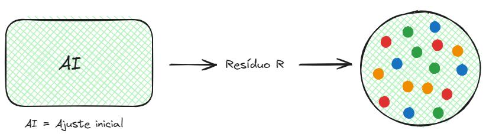
\includegraphics[width=0.8\textwidth]{Figuras/método pega o ajuste inicial e seleciona o resíduo para gerar novo ajuste a partir dele.png}
    \legend{Fonte: Própria autoria.}
    \label{figura15}
\end{figure}
Um novo modelo é então treinado para prever esse resíduo. Com base nesse novo modelo, um
novo resíduo é calculado, repetindo o processo dos passos anteriores.
\begin{figure}[htbp]
    \centering
    \caption{Novo ajuste é gerado a partir do outro ajuste e obtido um novo resíduo.}
    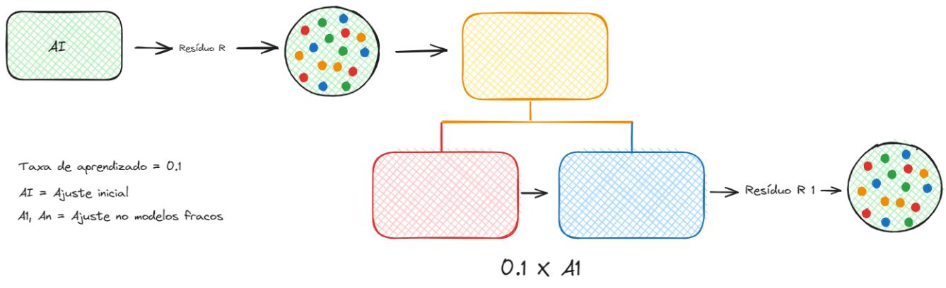
\includegraphics[width=0.8\textwidth]{Figuras/novo ajuste é gerado a partir do outro ajuste, e obtendo um novo resíduo.png}
    \legend{Fonte: Própria autoria.}
    \label{figura16}
\end{figure}
Um novo modelo é então criado e ajustado sobre o resíduo gerado pelo modelo anterior. Com base nesse novo modelo, um novo resíduo é calculado, como foi feito nos passos anteriores.

\begin{figure}[htbp]
    \centering
    \caption{Mais interação até que se chegue em um valor mínimo de erro possível.}
    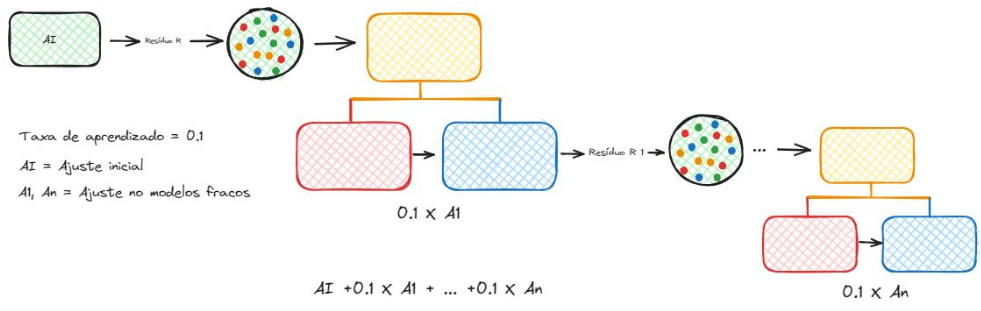
\includegraphics[width=0.8\textwidth]{Figuras/mais interação até que se chegue em um valor mínimo de erro possível.png}
    \legend{Fonte: Própria autoria.}
    \label{figura17}
\end{figure}
As interações são repetidas várias vezes, com o objetivo de minimizar o resíduo gerado pelos
modelos fracos, ou seja, até que o valor previsto e o valor real sejam a menor possível. O modelo
final é a soma dos ajustes de todos os modelos fracos.

\subsubsection{Light gradient boosting}
\textit{Light Gradient Boosting Machine} (LightGBM) é um algoritmo de aprendizado de
máquina desenvolvida pela Microsoft e disponibilizado como código aberto \textit{(open-source)}. Ele
se baseia no modelo de Gradient Boosting (GB), mas é mais rápido e eficiente que o GB
tradicional, que vimos na subseção anterior, e também que o XGBoost, que veremos
posteriormente.

O LightGBM utiliza um método de amostragem unilateral baseado em gradiente (GOSS
– \textit{Gradient basead One-Side Sampling}) para dividir as árvores, o que reduz significativamente
o uso de memória e melhora o desempenho. O GOSS seleciona instâncias de treinamento com
base na magnitude dos gradientes, mantendo as instâncias de gradientes grandes e realizando
uma amostragem aleatória das instâncias com gradientes pequenos. Isso preserva a precisão do
modelo ao reduzir o número de instâncias processadas, resultando em um treinamento mais
rápido. Além disso, ele emprega um crescimento baseado em folhas em vez de um crescimento
baseado em níveis, o que o torna mais rápido do que os algoritmos tradicionais que utilizam
crescimento em profundidade. 

Outra técnica inovadora usada pelo LightGBM é o EFB
(\textit{Exclusiva Feature Bundling}) \cite{ke2017lightgbm}. EFB agrupa característica mutuamente exclusivas em uma
única característica, ou seja, são eventos que não podem acontecer ao mesmo tempo, reduzindo
a dimensionalidade sem perda significativa de informação. Essa técnica é especialmente útil
quando há muitas características esparsas no conjunto de dados, pois reduz o espaço de memória necessário e acelera o processo de treinamento. Uma das grandes vantagens do
LightGBM é sua capacidade de lidar com conjuntos de dados em grande escala. Ele pode
processar milhões ou bilhões de registros com milhares de características, tornando-o ideal para
aplicações em que a escalabilidade é crucial.

\subsubsection{\textit{Extreme gradient boosting} (XGBoost)}
O \textit{}{Extreme Gradient Boosting} (XGBoost) é um algoritmo de aprendizado de
máquina baseado no método de \textit{Gradient Boosting}, e amplamente utilizado para resolver
problemas de classificação e regressão. O XGBoost aprimora o desempenho preditivo por meio
de uma abordagem iterativa, onde utiliza combinação ponderada uma sequência de modelos
fracos, como árvores de decisão, para corrigir erros cometidos nas iterações anteriores \cite{chen2016xgboost}. As
principais vantagens na utilização do algoritmo são:

• Regularização: XGBoost implementa regularização L1 e L2 para evitar overfitting, algo
que não é padrão em outras implementações de gradient boosting;

• Capacidade de lidar com valores ausentes: O XGBoost identifica e lida
automaticamente com valores faltantes durante o treinamento;

• Validação cruzada integrada: Ele realiza validação cruzada em cada iteração do
treinamento, o que facilita encontrar o número ótimo de iterações sem necessidade de
uma validação externa;

• Treinamento incremental: Permite interromper e retomar o treinamento, suportando o
batch training para cenários de grandes volumes de dados;

• Escalabilidade: O XGBoost pode ser escalado tanto verticalmente (processamento
paralelo em múltiplos núcleos) quando horizontalmente (distribuído em múltiplas
máquinas);

• Interrupção antecipada: Assim como modelos de rede neurais, oferece a possibilidade
de interromper o treinamento quando o modelo atinge o desempenho ótimo;

• Otimização de objetivo personalizada: Usuários podem definir funções de perda
personalizadas, permitindo ajuste mais refinado para problemas específicos;

• Poda de árvores: O XGBoost constrói árvores profundas e depois poda ramos ineficazes,
otimizando o modelo e evitando sobreajustes desnecessários.

Além disso, o XGBoost é conhecido por ser muito eficiente em termos computacionais,
utilizando técnicas como \textit{out-of-core computation} \cite{schiara2023detailed} para lidar com grandes conjuntos de
dados, e suporte a processamento paralelo, o que o torna uma escolha ideal para problemas
de aprendizado de máquina que demandam de alta performance.

\subsection{Aprendizado profundo (\textit{Deep Learning})}
O \textit{Deep Learning} é uma subárea do aprendizado de máquina baseada em redes
neurais artificiais com múltiplas camadas, capazes de aprender representações complexas a a
partir dos dados. Esses modelos são inspirados na estrutura e no funcionamento do cérebro
humano, particularmente na forma como os neurônios se conectam e processam informações.
O \textit{Deep Learning} tem sido aplicado em diversas tarefas complexas da inteligência artificial, como
visão computacional, processamento de linguagem natural (\textit{Natural Language Processing} –
NLP), reconhecimento de fala e, mais recentemente, no desenvolvimento de grandes modelos
de linguagem (\textit{Large Language Models} – LLMs).

Os primeiros estudos relacionados às redes neurais iniciaram por volta 1943,
quando o neurofisiologista Warrem McCulloch e o matemático Walter Pitts \cite{palm1986warren} apresentaram
um dos primeiros modelos matemáticos inspirados no funcionamento simplificada do neurônio
baseado em princípios da lógica proposicional, estabelecendo fundamentos importantes para o
desenvolvimento das redes neurais artificiais \cite{yang2016propositional}. 

Do ponto de vista biológico, o neurônio é
uma célula do sistema nervoso composta por um corpo celular (soma), que contém o núcleo,
além de ramificações chamadas dendritos, responsáveis por receber sinais de outros neurônios,
e uma extensão longa denominado axônio, responsável por transmitir sinais elétricos. O axônio
pode apresentar ramificações chamadas telodendros, cujas extremidades formam os terminais
sinápticos, onde ocorre a comunicação com outros neurônios por meio das sinapses.

A organização dos neurônios no cérebro é um campo de investigação científica bastante ativa.
Estudos indicam que, especialmente no córtex cerebral, os neurônios tendem a se organizar em
estruturas em camadas, característica que inspirou o desenvolvimento das arquiteturas de redes
neurais artificiais utilizadas atualmente. 

As redes neurais biológicas desempenham papel
fundamental no funcionamento do sistema nervoso, sendo responsáveis por processos como
percepção, controle motor, aprendizado e raciocínio. Inspiradas nesse mecanismo biológicos,
as redes neurais artificiais buscam reproduzir, de forma simplificada, alguns desses princípios
para resolver problemas computacionais.

O modelo de neurônio artificial proposto por
McCulloch e Pitts consiste em uma estrutura simples que recebe um ou mais sinais de entrada e produz um único sinal de saída. Cada entrada é multiplicada por um peso, que representa a
força da conexão. Em seguida, os valores ponderados são somados juntamente com um termo
de viés (bias), e o resultado é aplicado a uma função de ativação, produzindo a saída do
neurônio. Redes neurais artificiais são, portanto, compostas por um conjunto de neurônios
artificiais organizados em camadas, capazes de aprender representações complexas dos dados.
Essas redes são amplamente utilizadas em tarefas como classificação, regressão e
reconhecimento de padrões, sendo a base de muitos dos avanços recentes em Inteligência
Artificial.

\subsection{Métricas de Classificação}
A avaliação do desempenho de modelos de aprendizado de máquina é uma etapa
fundamental no processo de desenvolvimento de sistemas de inteligência artificial. Para isso,
são utilizadas funções matemáticas conhecidas como métricas de avaliação, que permitem
medir o desempenho do modelo em relação aos dados reais. Em problemas de classificação,
uma das ferramentas mais utilizadas para análise do desempenho do modelo é a matriz de
confusão. A matriz de confusão é uma tabela que compara os valores previstos pelo modelo
com os valores reais do conjunto de dados. Dessa forma, ela permite visualizar quantas
previsões foram realizadas corretamente e quantas foram classificadas de forma incorreta. Essa
matriz apresenta a decomposição das previsões em quatro categorias principais:

• Verdadeiro positivo (VP): quando o modelo prevê corretamente a classe
positiva;

• Verdadeiro negativa (VN): quando o modelo prevê corretamente a classe
negativa;

• Falso Positivo (FP): quando o modelo classifica uma instância como
positiva, mas na realidade ela pertence à classe negativa;

• Falso negativo (FN): quando o modelo classifica uma instância como
negativa, mas na realidade ela pertence à classe positiva.

A partir desses valores, diferentes métricas podem ser calculadas para avaliar o desempenho do
modelo. É importante destacar que, normalmente, um modelo não é avaliado por apenas uma
métrica, mas por um conjunto dela, pois cada métricas fornece uma perspectiva diferente sobre
o desempenho do modelo. Além disso, as métricas utilizadas dependem do tipo de problema abordado. Modelos de regressão, por exemplo, utilizam métricas diferentes das aplicadas em
problemas de classificação. Como este trabalho aborda um problema de classificação, serão
utilizadas métricas específicas para este tipo de modelo.


\subsubsection{Acurácia}
A acurácia é uma das métricas mais utilizadas na avaliação de modelos de classificação. Ela
mede a proporção de previsões corretas em relação ao total de previsões realizadas pelo modelo.
Em outras palavras, a acurácia representa o percentual de classificação corretas considerando
tanto as classes positivas quanto as negativas. A fórmula da acurácia é definida por:
\begin{equation}
    Acurácia = \frac{VP + VN}{VP + VN + FP + FN}
    \label{eq:40}
\end{equation}
\subsubsection{Precisão}
A precisão mede a proporção de previsões positivas que realmente pertencem à classe positiva.
Essa métricas é especialmente importante em situações onde falso positivos precisam ser
minimizados. Um falso positivo (FT) ocorre quando o modelo classifica uma instância como
positiva, mas ela pertence à classe negativa. A precisão é calculada da seguinte forma:
\begin{equation}
    Precisão = \frac{VP}{VP + FP}
    \label{eq:41}
\end{equation}
\subsubsection{Revocação (Recall)}
 A revocação, também conhecida como recall ou sensibilidade, mede a capacidade do modelo
de identificar corretamente as instâncias positivas. Essa métrica avalia quantos dos exemplos
que realmente pertencem à classe positiva foram corretamente identificados pelo modelo. Um
falso negativo (FN) ocorre quando um exemplo positivo é classificado incorretamente como
negativo. A revocação é definida pela seguinte equação:
\begin{equation}
    Precisão = \frac{VP}{VP + FN}
    \label{eq:42}
\end{equation}
\subsubsection{F1-Score}
O F1 Score é uma métrica que combina precisão e revocação em um único valor. Essa métrica
corresponde à média harmônica entre essas duas medidas, sendo particularmente útil quando
há um desequilíbrio entre as classes. Esse métrica busca equilibrar os erros associados a falsos
positivos (FP) e falsos negativos (FN), fornecendo uma medida mais robusta do desempenho
do modelo. Sua fórmula é dada por:
\begin{equation}
    F1\ Score = 2 \times \frac{Precisão \times Revocação}{Precisão + Revocação}
    \label{eq:43}
\end{equation}
\subsubsection{Matriz de Confusão}
A matriz de confusão é umas das métricas mais utilizadas na avaliação de modelos de
classificação supervisionada, pois organiza os resultados preditos pelo modelo em relação às
classes reais observadas. Em vez de fornecer apenas uma medida global de desempenho, como
a acurácia, ela permite analisar individualmente os acertos e erros do classificador,
identificando quais classes estão sendo confundidas com maior frequência. 

Essa característica
é especialmente importante em problemas com classes desbalanceadas, nos quais uma alta
acurácia pode ocultar falhas relevantes do modelo. Em uma classificação binária, a matriz de
confusão é formada por quatro elementos fundamentais: verdadeiro positivo (TP), verdadeiro
negativo (TN), falso positivo (FT) e falso negativo (FN). Esses valores sevem de base para o
cálculo de métricas derivadas, como precisão, recall e F1-score, que aprofundam a análise do
comportamento do modelo.

Dessa forma, a matriz de confusão não apenas informa se o modelo
acertou ou errou, mas também mostra o tipo de erro cometido, o que é útil para justes posteriores
no treinamento e na escolha de limiares de decisão. Além da classificação binária, a matriz de
confusão também pode ser aplicada em problemas multiclasse, assumindo a forma de uma
tabela $N\times N$, em que $N$ representa o número de classes do problema. Nesses casos, cada linha
e coluna indicam, respectivamente, as classes reais e as classes preditas, permitindo visualizar
de maneira clara quais categorias o modelo consegue distinguir com precisão e quais
apresentam maior sobreposição \cite{meyerbaese2014foundations}.

\chapter{Resultados e Discussões}
Neste capítulo são apresentados e discutidos os procedimentos adotados para o
desenvolvimento do modelo de aprendizado de máquina destinado à classificação de circuitos
equivalentes aplicados à EIS.
Inicialmente, estabeleceu-se como objetivo a construção de um conjunto de dados
adequado para o treinamento da rede neural e de outros algoritmos de aprendizado de máquina.
Foi aplicado diferentes configurações de circuitos equivalentes, correspondentes às classes
utilizadas no processo de classificação supervisiona.

Entretanto, a quantidade de dados
experimentais disponível mostrou-se insuficiente para atender às necessidades de treinamento
dos modelos, especialmente considerando a diversidade. Com o intuito de superar essa
limitação, foi empregada a ferramenta \textit{Automaterials} \cite{mouta2025automaterials}, desenvolvida pelo professor Doutor Rodolpho Mouta, que possibilita a
geração sintética de EIS a partir de parâmetros previamente definidos.

A utilização dessa
ferramenta permitiu a criação de uma base de dados robusta e balanceada, composta por
espectros sintéticos representativos de diferentes fenômenos eletroquímicos observados
experimentalmente. Para cada modelo de circuito foram gerados 10 mil espectros, conforme
apresentado na Tabela \ref{tab:1}.

\begin{table}[htb]
    \centering
    \caption{Relação dos circuitos e a quantidade de espectros utilizado no treinamento dos modelos de \textit{Machine Learning}}
    \label{tab:1}
    \begin{tabular}{ccc}
        \hline
        Circuitos & Quantidade de Dados Gerados \\
        \hline
        RC & 10.000 \\         
        RQ & 10.000 \\
        RQRQ\_RQ & 10.000 \\
        RQRQ\_RQ\_Q & 10.000 \\
        RQ\_Q & 10.000 \\
        RQ\_RQ & 10.000 \\
        R\_L\_RQ & 10.000 \\
        R\_L\_RQ\_Q & 10.000 \\
        R\_L\_RQ\_RQ & 10.000 \\
        R\_RQ & 10.000 \\
        R\_RQ\_RQ & 10.000 \\   
        \hline
    \end{tabular}
    \legend{Fonte: Autoria Própria.}
\end{table}

Os dados sintéticos foram gerados a partir de onze modelos de circuitos
equivalentes amplamente utilizados para representar sistemas eletroquímicos reais. Cada
modelo representa uma combinação específica de elementos, tais como resistores ($R$),
indutores ($L$), capacitiva ($C$) e elementos de fase constante ($Q$), conectados em série ou em
paralelo. Essas configurações permitem descrever diferentes fenômenos físicos associados aos
processos eletroquímicos, incluindo resistência de ôhmica da solução, transferência de carga,
comportamento capacitivo ideal, processo difusivos e efeitos indutivos observados em
determinadas condições experimentais.

O processo de geração dos espectros exigiu a definição
prévia dos parâmetros característicos de cada circuito, incluindo frequência, resistência,
indutância e os parâmetros do elemento de fase constante (CPE - \textit{Constante Phase Element}), representados pela constante $T$ e pelo expoente $p$, como podemos
ver na equação \eqref{eq:31}. 

Além disso, definiu-se o intervalo de variação da frequência em décadas
logarítmicas, iniciando com 30 pontos por décadas. Os parâmetros de entrada empregados na geração
sintética dos dados encontram-se resumidos na Tabela \ref{tab:2}.

\begin{table}[htb]
	\caption{Relação dos inputs dos parâmetros para geração dos dados de IES.}
	\label{tab:2}
	\centering
	\resizebox{\textwidth}{!}{%
		\begin{tabular}{lccccccc}
			\toprule
			\multirow{2}{*}{\textbf{Circuitos}} & \multicolumn{3}{c}{\textbf{Dentro do $RC/RQ$}} & \multicolumn{3}{c}{\textbf{Fora do $RC/RQ$}} & \multirow{2}{*}{\textbf{$L(H)$}} \\
			\cmidrule(lr){2-4} \cmidrule(lr){5-7}
			& $R\,(\Omega)$ & $T$ & $P$ & $R\,(\Omega)$ & $T$ & $P$ & \\
			\midrule
			RC          & $10-10^{10}$ & $10^{-13}-10^{-4}$ & --            & --           & --                  & --            & --                 \\
			RQ          & $10-10^{10}$ & $10^{-13}-10^{-4}$ & $0.4-1.0$     & --           & --                  & --            & --                 \\
			RQRQ\_RQ    & $10-10^{10}$ & $10^{-13}-10^{-4}$ & $0.4-1.0$     & --           & --                  & --            & --                 \\
			RQRQ\_RQ\_Q & $10-10^{10}$ & $10^{-13}-10^{-4}$ & $0.4-1.0$     & --           & $10^{-9}-10^{-4}$   & $0.5-0.9$     & --                 \\
			RQ\_Q       & $10-10^{10}$ & $10^{-13}-10^{-4}$ & $0.4-1.0$     & --           & $10^{-9}-10^{-4}$   & $0.5-0.9$     & --                 \\
			RQ\_RQ      & $10-10^{10}$ & $10^{-13}-10^{-4}$ & $0.4-1.0$     & --           & --                  & --            & --                 \\
			R\_L\_RQ    & $10-10^{10}$ & $10^{-13}-10^{-4}$ & $0.4-1.0$     & $1-10^{3}$   & --                  & --            & $10^{-7}-10^{-4}$  \\
			R\_L\_RQ\_Q & $10-10^{10}$ & $10^{-13}-10^{-4}$ & $0.4-1.0$     & $1-10^{3}$   & $10^{-9}-10^{-4}$   & $0.5-0.9$     & $10^{-7}-10^{-4}$  \\
			R\_L\_RQ\_RQ& $10-10^{10}$ & $10^{-13}-10^{-4}$ & $0.4-1.0$     & $1-10^{3}$   & --                  & --            & $10^{-7}-10^{-4}$  \\
			R\_RQ       & $10-10^{10}$ & $10^{-13}-10^{-4}$ & $0.4-1.0$     & $1-10^{3}$   & --                  & --            & --                 \\
			R\_RQ\_RQ   & $10-10^{10}$ & $10^{-13}-10^{-4}$ & $0.4-1.0$     & $1-10^{3}$   & --                  & --            & --                 \\
			\bottomrule
		\end{tabular}%
	}
	\legend{Fonte: Autoria própia.}
\end{table}

A definição dos intervalos de cada parâmetro buscou reproduzir condições
fisicamente plausíveis encontradas na literatura, com diversos parâmetros de impedância
podem variar ao longo de várias ordens de grandeza, optou-se pela utilização predominante de
amostras no espaço de busca e evitando a concentração excessiva de dados em determinadas
regiões. 

As resistências presentes no subcircuitos ($RQ$), normalmente associadas à resistência
de transferência de carga ou à resistência de polarização da interface eletroquímica, foram
definidas no intervalo de $10\,\Omega$ a $10^{10}\,\Omega$. Essa ampla faixa permite representar desde sistemas
altamente condutivos até materiais com elevadas resistências elétrica.

Para esses parâmetros foi
utilizada amostragem logarítmica, garantido representação equilibrada ao longo de todas as
ordens de grandeza consideradas. O elemento de fase constante ($Q$), como mencionado
anteriormente, é caracterizado pelos parâmetros $T$ e $P$. O parâmetro $T$ está relacionado à
magnitude da admitância do elemento e pode ser associado a fenômenos como capacitância de dupla camada elétrica, rugosidade superficial, heterogeneidade da interface e processo
difusivos.

Quando inserido em um subcircuito ($RQ$), o parâmetro $T$ foi definido entre $10^{-13}$ e $10^{-4}$, utilizando amostragem logarítmica. Essa faixa permite representar desde interface com baixa resposta capacitiva até sistema com comportamento fortemente capacitivo. O expoente $P$ do elemento $Q$ controla o grau de dispersão da frequência do sistema e o desvio em relação ao comportamento de um capacitor ideal. Quando $P$ assume o valor de 1, o elemento apresenta comportamento capacitivo ideal. 
Valores menores indicam diferentes níveis de
heterogeneidade ou efeitos difusivos.

Para os elementos $Q$ inseridos em subcircuitos ($RQ$), o
parâmetro $P$ varia entre $0.4$ e $1.0$, utilizando amostragem linear, abrangendo desde o
comportamento próximo ao modelo de Warburg até respostas capacitivas quase ideais. Nos
casos que o elemento $Q$ aparece isoladamente no circuito, sem associação direta a um resistor
em paralelo, foram adotadas faixas mais restritas.

O parâmetro $T$ varia entre \(10^{-9}\) e $10^{-4}$,
enquanto o parâmetro $P$ foi definido entre $0.5$ e $0.9$. Essas restrições foram estabelecidas para
representar fenômenos difusivos e respostas da interfacei mais específicas, mantendo coerência
física com os comportamentos normalmente observados em espectros experimentais.

As
resistências externas aos subcircuitos $RQ$, geralmente associadas à resistência ôhmica do
eletrólito ou a componentes em série do sistema eletroquímico, foram definidas no intervalo de
$1\,\Omega$ a $1000\,\Omega$, também utilizando amostragem logarítmica. Essa faixa contempla desde soluções altamente condutivas até sistemas com resistência ôhmica moderada.

Os elementos indutivos
foram incluídos nos circuitos $R-L-RQ,\; R-L-RQ-Q,\; R-L-RQ-RQ$ para
representar efeitos observados principalmente em altas frequências, frequentemente associados
à instrumentação, cabos de conexão ou característica geométricas da célula eletroquímica. Para esses elementos, adotou-se uma faixa de valores entre \(10^{-7}\) e \(10^{-4}\), com amostragem
logarítmica.

A utilização da amostragem logarítmica para resistências, indutância e parâmetros
$T$ mostrou-se particularmente importante devido à natureza desses parâmetros, que podem
varias por diversas ordens de grandeza. Caso fosse empregada uma distribuição linear, a maior
parte das amostras ficaria concentradas nas regiões de valores elevados, reduzindo
significativamente a representatividade dos valores menores. Dessa forma, os intervalos
adotados e os métodos de amostragem empregados possibilitaram a geração de espectros
sintéticos capazes de representar uma ampla variedade de comportamentos eletroquímicos,
fornecendo uma base consistente para o treinamento.

Após a definição da estratégia de geração dos espectros sintéticos e a validação de
que os dados produzidos apresentavam comportamentos fisicamente compatível com os EIS surgiu a necessidade de desenvolver uma infraestrutura capaz de armazenar e gerenciar o grande volume de dados gerados. Considerando que cada espectro é composto por uma
estrutura matricial contendo informações de frequência, impedância real e impedância
imaginária, optou-se pela aplicação de técnicas de Engenharia de Dados para garantir o
armazenamento eficiente e organizado dessas informações.

Para isso, foi construído um
servidor dedicado baseado em Linux, projetado especificamente para suportar o
armazenamento e o processamento dos dados de EIS. Entre as alternativas avaliadas para
persistência dos dados, foi escolhido o MongoDB, um sistema de gerenciamento de banco de
dados NoSQL orientado a documentos. A escolha foi motivada pela sua flexibilidade na
modelagem de dados, facilidade de integração com aplicações desenvolvidas em \textit{Python},
capacidade de lidar com estruturas semiestruturadas e pelo fato de ser uma solução \textit{Open Source}
amplamente utilizada em aplicações científicas e de análise de dados.

Com a infraestrutura do
servidor estabelecida, tornou-se necessário desenvolver uma camada de comunicação entre os
programas de geração e análise dos espectros e o banco de dados. Para atender essa necessidade,
foi desenvolvida uma biblioteca especifica denominada CISD (\textit{Connection Impedance Storage
and Data Analysis}), responsável por abstrair as operações de conexão, inserção, consulta e
recuperação dos espectros armazenados. A biblioteca foi projetada considerando as
particularidades dos dados de EIS, permitindo manipular de forma eficiente as informações
espectrais e os metadados associados a cada circuito equivalente. Todo o ambiente
computacional foi desenvolvido utilizando a linguagem de programação Python. 

Além dos
scripts responsáveis pela geração dos espectros sintéticos, foram implementados módulos
específicos para armazenamento, validação, processamento e recuperação dos dados. Essa
arquitetura permitiu criar um fluxo integrado, desde a geração dos espectros até sua
disponibilização para etapas de treinamento e validação dos modelos de aprendizado de
máquina. A adoção dessa infraestrutura proporcionou não apenas um ambiente adequado para
armazenamento dos milhares de espectros gerados, mas também garantiu escalabilidade para
futuras expansões da base de dados, e (que de fato ocorreram com adicionando ruídos nos
espectro) possibilitando a inclusão de novos modelos de circuitos equivalentes e de dados
experimentais reais. 

Com a base de dados consolidada e a infraestrutura de armazenamento
devidamente estabelecida, o próximo passo consistiu no desenvolvimento dos modelos de
aprendizado profundo. Com a geração dos espectros sintéticos concluída, a validação física
dos dados realizada e a infraestrutura de armazenamento devidamente estabelecida, tornou-se
possível iniciar a etapa de desenvolvimento dos modelos de aprendizado da rede neural. 

O objetivo era construir a rede neural convolucional capaz de identificar automaticamente o circuito equivalente associado a cada espectro de impedância eletroquímico. Com mencionado
anteriormente, os espectros utilizados no treinamento foram armazenados no banco MongoDB,
organizadas em coleções independentes, cada uma representando uma topologia distinta de
circuito equivalente, como mostra na tabela 1. As onzes configurações de circuito elétricos,
correspondendo às classes do problema de classificação supervisionado. 

Para cada classe foram
recuperados até 10.000 amostras totalizando um conjunto de dados, aproximadamente 110.000
espectros utilizadas no treinamento e avaliação do modelo. Os primeiros treinamentos foram
conduzidos utilizando os espectros em sua forma original, sem quaisquer procedimentos de
normalização, padronização ou alguma forma de escalonamento.

Nessa configuração, os
valores de frequência, impedância real e impedância imaginária apresentavam diferenças
significativas de magnitude, fazendo com que determinadas características dominassem o
processo de aprendizado da rede neural. Como consequência, os resultados obtidos mostraram-
se insatisfatórias, apresentando taxas de erro entre $70\%$ e $80\%$. 

Diante desse cenário, tornou-
se necessária a implementação de uma etapa de pré-processamento dos dados. A estratégia
adotada foi baseada no trabalho de Buteau e Dahn \cite{buteau2019analysis}. Nesse estudo, os autores demonstram
que a normalização adequada dos espectros de impedância é fundamental para melhorar a
estabilidade do treinamento e a capacidade de generalização dos modelos de aprendizado de
máquina. 

O trabalho introduz o conceito de distribuição a priori para os parâmetros dos circuitos
equivalentes, assumindo que cada parâmetro pode ser modelado por uma distribuição gaussiana
independente caracterizada por um valor médio e um desvio padrão. Segundo os autores, a
definição essas distribuições tornam-se significativamente mais simples quando os espectros
são previamente normalizados de acordo com duas condições fundamentais: O valor absoluto máximo da impedância deve ser igual a 1 e a média do logaritmo da frequência deve ser igual a zero.

A primeira condição elimina diferença de escala entre espectros obtidos em diferentes sistemas
ou condições experimentais. A segunda centraliza a distribuição de frequência em escala
logarítmica, tornando os espectros mais comparáveis e facilitando o aprendizado dos padrões
físicos relevantes. Com base nessa metodologia, foi desenvolvido um procedimento de
normalização específico para os espectros utilizados neste trabalho, adaptando os princípios
propostos por Buteau e Dahn \cite{buteau2019analysis} às características dos dados disponíveis.

Inicialmente, o vetor
de frequência foi transformado para escala logarítmica por meio de aplicação do algoritmo,
conforme a equação \eqref{eq:44}:
\begin{equation}
\omega_i = \ln(f_i), \quad i = 1, 2, \ldots, N
\label{eq:44}
\end{equation}

A seguir, em vez de subtrair a média aritméticas dos logaritmos – como proposto originalmente por Buteau e Dahn \cite{buteau2019analysis}, que garante que a média do logaritmo das frequências normalizadas seja
zero, optou-se pela divisão pela mediana da distribuição logarítmica, conforme a equação \eqref{eq:45}:
\begin{equation}
\omega_i^{\mathrm{norm}} =
\frac{\ln(f_i)}
{\operatorname{mediana}\left(\{\ln(f_j)\}_{j=1}^{N}\right)}
\label{eq:45}
\end{equation}

Essa escolha foi motivada pela maior robustez da mediana em relação a valores extremos.
Diferentemente da média aritmética, a mediana não é influenciada por pontos atípicos presentes
nos extremos dos espectros de frequência, que são comuns em medições de impedância
eletroquímica realizadas em faixas de frequência muito amplas.

Com essa abordagem, o
resultado da normalização garante que a mediana dos logaritmos normalizados seja igual a 1,
preservando a proporção por Buteau e Dahn \cite{buteau2019analysis}, por sua vez, garante que a média seja igual a
zero por meio de uma operação de recentramento aditivo. Ambos as estratégias atendem ao
mesmo objetivo geral de reduzir os efeitos de escala e deslocamento entre espectros distintos,
diferindo apenas no estimador de posição central utilizado e na operação matemática
empregada. 

Posteriormente, os valores de impedância real e imaginária foram combinados para
formar a impedância complexa, equação \eqref{eq:46}:
\begin{equation}
Z_{\max}=\max_i |Z_i|
=\max_i \sqrt{Z_{\mathrm{re},i}^{2}+Z_{\mathrm{im},i}^{2}},
\label{eq:46}
\end{equation}
e utilizado como fator de normalização, em acordo com a condição proposta por Buteau e Dahn \cite{buteau2019analysis}, equação \eqref{eq:47}:
\begin{equation}
Z_i^{\mathrm{norm}}
=\frac{Z_i}{Z_{\max}}.
\label{eq:47}
\end{equation}
Dessa forma, todos os pontos do espectro passaram a possuir magnitude relativa à impedância
máxima observada, garantindo que max
$\max_i |Z_i^{\mathrm{norm}}| = 1$, e que os dados permanecessem em uma
faixa padronizada e comparável entre diferentes amostras. Por fim, as três grandezas
normalizadas – frequência logarítmica, parte real e parte imaginária a impedância – foram
concatenadas para forma o vetor de entrada da rede neural, equação \eqref{eq:48}:
\begin{equation}
\chi=
\left[
\omega_1^{\mathrm{norm}},\ldots,\omega_N^{\mathrm{norm}},
\operatorname{Re}\!\left(Z_1^{\mathrm{norm}}\right),\ldots,
\operatorname{Re}\!\left(Z_N^{\mathrm{norm}}\right),
\operatorname{Im}\!\left(Z_1^{\mathrm{norm}}\right),\ldots,
\operatorname{Im}\!\left(Z_N^{\mathrm{norm}}\right)
\right]
\in \mathbb{R}^{3N}
\label{eq:48}
\end{equation}

Para os espectros utilizados neste trabalho, compostos por $N$ = 181 pontos de frequência, o
vetor resultante possui dimensão $3 \times181 = 543$, que correspondendo ao formato de entrada
da camada inicial da rede neural convolucional. Ao final da etapa de pré-processamento, foi
obtida uma matriz de entrada com dimensão (110000, 543, 1), adequada para utilização em
uma rede neural convolucional (CNN) unidimensional. Os rótulos foram convertidos para
codificação categórica para codificação categórica (one-hot enconding), produzindo uma
matriz com formato de (110000, 11), onde 11 corresponde ao número de topologias de
circuitos equivalente consideradas no problema de classificação.

A arquitetura desenvolvida consiste em uma CNN unidimensional (Conv1D), projetada
para identificar padrões característicos presentes nos espectros de impedância eletroquímica
normalizada. A rede possui uma camada de entrada com dimensão (543, 1), seguida por duas
camadas convolucionais contendo 16 e 32 filtros, respectivamente, ambas utilizando a função
de ativação \textit{ReLU} (Rectified linear Unit). Essa função de ativação, definida como $f(x)$ = $max(0,x)$, introduz não-linearidade ao modelo sem comprometer a eficiência computacional
do treinamento. 

Após essas etapas, aplica-se uma camada de MaxPooling para redução
dimensional e extração das características mais relevantes, reduzindo pela metade a dimensão
temporal da representação. Na sequência, uma terceira camada convolucional contendo 64
filtros é utilizada para aprofundar a extração de atributos espectrais, capturando padrões de
maior complexidade e abstração. Uma nova operação de MaxPooling é aplicada antes da etapa
de achatamento dos dados (Flatten), que converte a representação multidimensional em um
vetor unidimensional de 8.640 elementos.

As características extraídas pelas camadas
convolucionais são então processadas por uma camada totalmente conectada (Dense) contendo
128 neurônios com ativação ReLu, responsável por combinar globalmente os atributos
aprendidos. Finalmente, a camada de saída utiliza 11 neurônios com função de ativação
Softmax, que transforma os valores de saída em probabilidades normalizadas – isto é, valores
entre 0 e 1 cuja soma é sempre igual a 1 – associadas a cada uma das classes de circuitos
equivalentes. A classe predita corresponde ao neurônio de maior probabilidade. O modelo foi
compilado utilizando o otimizador Adam e a função de perda categorical crossentropy,
amplamente empregada em problemas de classificação multiclasse com rótulos em formato
one-hot.

Os dados foram divididos em $80\%$ para treinamento e $20\%$ para teste. Dentro do
conjunto de treinamento foi reservada uma parcela adicional de $20\%$ para validação,
permitindo monitorar a capacidade de generalização do modelo ao longo das épocas sem
contaminação pelo conjunto de teste. O treinamento foi configurado para até 3 mil épocas,
utilizando lotes de 32 amostrar (batch size). Para evitar sobreajuste (overfitting) e preservar a
melhor configuração encontrada durante o treinamento, foram empregados dois mecanismos
de controle:

• Early Stopping: interrompe automaticamente o treinamento quando não são observadas
melhorias na perda de validação (val\_loss) durante um número pré-definido de época
consecutivas (paciência de 10 épocas), evitando iterações desnecessários após a
convergência.

• Model Checkpoint: armazena automaticamente em disco a versão do modelo que
apresenta o menor valor de perda de validação observado até o momento, garantindo
que o modelo salvo ao final do treinamento corresponda ao melhor estado alcançado,
independentemente de eventuais oscilações posteriores.

A evolução do treinamento foi acompanhada por meio das métricas de acurácia e função de
perda (loss), calculadas tanto para os conjuntos de treinamento quanto para validação ao
longo das 3 mil épocas executadas. A Figura~\ref{figura18} apresenta as curvas de acurácia do conjunto de treinamento (linha azul)
e do conjunto de validação (linha laranja) ao longo das épocas.

\begin{figure}[htbp]
    \centering
    \caption{Evolução da acurácia de treinamento e de validação ao longo das épocas
de treinamento da rede neural convolucional.}
    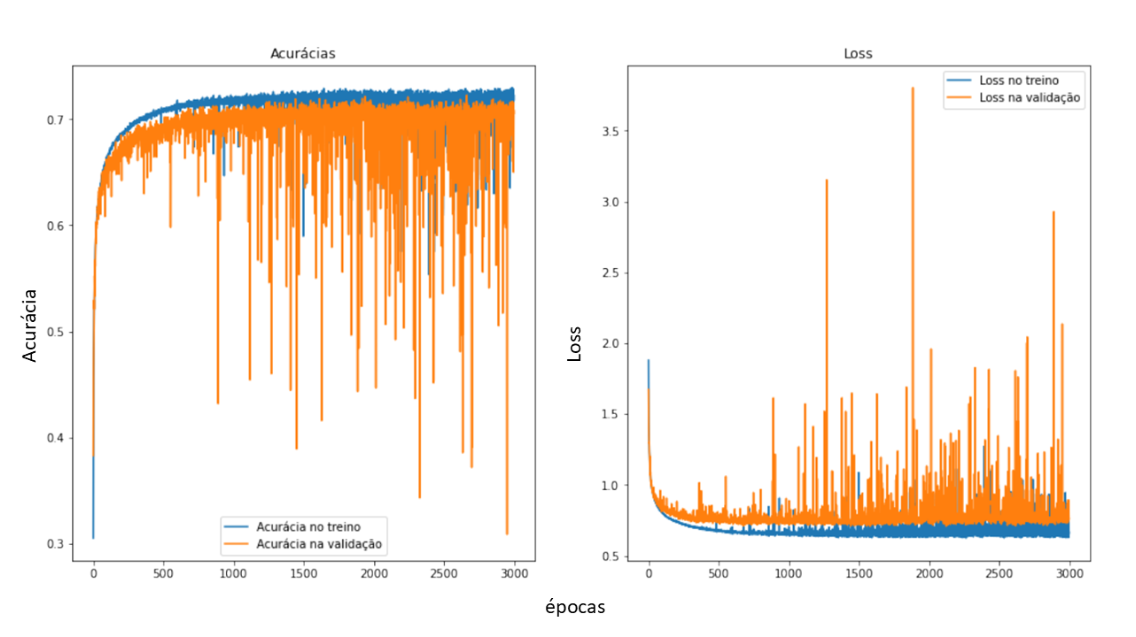
\includegraphics[width=0.9\textwidth]{Figuras/evolução da acurácia de treinamento e de validação ao longo das épocas de treinamento da rede neural convolucional.png}
    \legend{Fonte:Imagem gerada pelo algoritmo de treinamento.}
    \label{figura18}
\end{figure}

Observa-se um crescimento rápido e consistente da acurácia de treinamento nas
primeiras centenas de épocas, partindo de valores próximos a $30\%$ e estabilizando-se em torno
de $71\%$ ao longo do restante do treinamento. A curva de validação acompanha a tendência
geral de crescimento, porém com oscilação mais acentuadas, incluindo quedas pontuais
abruptas em algumas épocas. Esse comportamento é característico de treinamentos de longa
duração com o otimizador Adam, em que picos esporádicos na função de perda – provocados
por lotes (batches) de maior dificuldade – afetam momentaneamente a acurácia de validação,
sendo rapidamente corrigidos nas épocas seguintes. De modo geral, o modelo atingiu acurácia
de treinamento de aproximadamente $71.9\%$ e acurácia de validação de aproximadamente de
$70,6\%$ nas épocas finais, evidenciando boa capacidade de generalização e ausência de
sobreajuste significativo.

A curva de perda de treinamento apresenta decréscimo suave e
progressivo, saindo de valores próximos a 1.8 nas primeiras épocas e convergindo para
aproximadamente 0.66 ao final das 3 mil épocas. A curva de perda de validação, por sua vez,
exibe picos isolados que chegam a ultrapassar valores de 3.0 em determinados momentos,
refletindo instabilidades pontuais durante o processo de otimização. Ainda assim, o
comportamento médio da curva de validação também apresenta tendência de decréscimo,
estabilizando-se em torno de 0.76 nas épocas finais. A diferença entre a perda de treinamento e
a de validação, indicando que o modelo não decorou os dados de treinamento, mas aprendeu
padrões suficientes generalizáveis.

A Figura~\ref{figura19} apresenta o histórico completo do treinamento
com todos as quatros métricas sobrepostas em um único gráfico: perda de treinamento (\textit{loss},azul), acurácia de treinamento (\textit{accuracy}, laranja), perda validação (\textit{val\_loss}, verde) e  de validação (\textit{val\_accuracy}, vermelho).

\begin{figure}[htbp]
    \centering
    \caption{Histórico consolidado de treinamento: perda e acurácia de treinamento e validação ao longo das épocas.}
    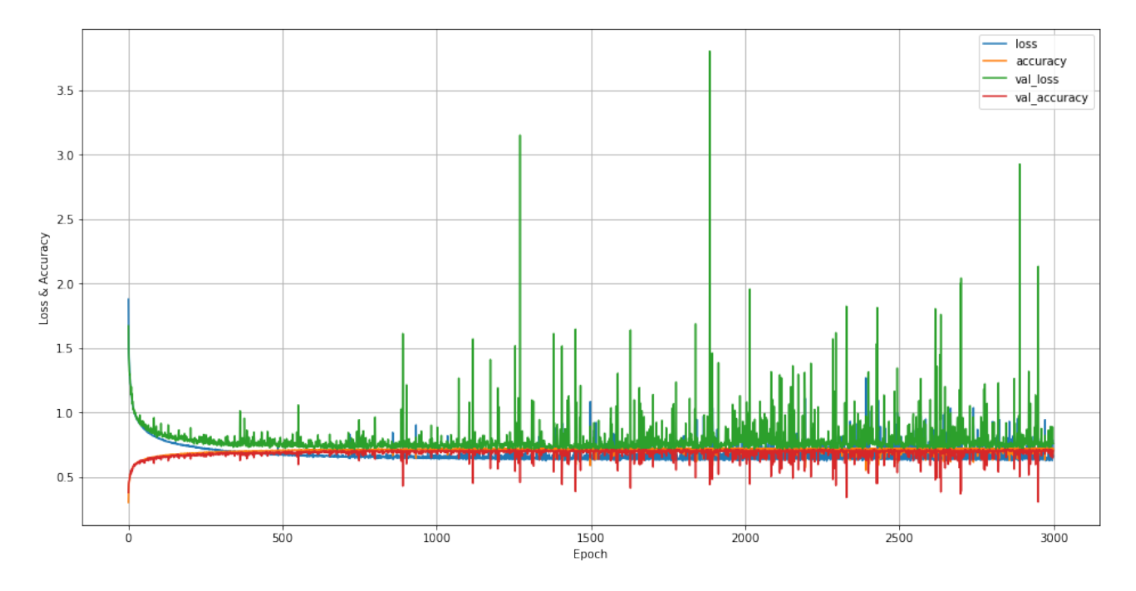
\includegraphics[width=0.9\textwidth]{Figuras/historico_treinamento.png}
    \legend{Fonte: Imagem gerada pelo algoritmo de treinamento.}
    \label{figura19}
\end{figure}

O gráfico confirma visualmente os comportamentos descritos anteriormente e evidência
com clareza o contraste entre as curvas de treinamento – mais suaves e estáveis – e as curvas
de validação – com oscilações mais pronunciadas, especialmente na perda de validação (verde).
Nota-se que, a partir de aproximadamente 500 épocas, todas as métricas passam a variar em
torno de valores relativamente estáveis, indicando que o modelo atingiu sua capacidade máxima
de aprendizado com a arquitetura e os dados disponíveis. Além da acurácia, foram calculadas
métricas complementares de avaliação para o conjunto de teste, incluindo Precisão (\textit{Precision}),
Revocação (\textit{Recall}) e \textit{F1-score}, toda calculadas com média ponderada pela proporção de cada
classe (\textit{wieghter average}). Os resultados obtidos estão indicados na tabela~\ref{tab:metricas_desempenho}.

\begin{table}[htb]
\caption{Métricas de classificação de desempenho do modelo avaliado}
\label{tab:metricas_desempenho}
\centering

\begin{tabular}{lc}
\toprule
\textbf{Métrica} & \textbf{Valor (\%)} \\
\midrule
Precisão  & 74,17 \\
Recall    & 70,84 \\
F1-Score  & 70,93 \\
\bottomrule
\end{tabular}

\legend{Fonte: Autoria própria.}
\end{table}

Esses valores demonstram desempenho consistente e equilibrado para a tarefa de
identificação automática dos circuitos equivalentes. A precisão ligeiramente superior ao
recall indica que, quando o modelo classifica um espectro como pertencente e determinada
topologia, essa predição tende a estar correta em 74\% dos casos: já o recall 70.8\% indica
que, do tal de espectros de cada classe, o modelo identificou corretamente aproximadamente
71\% deles. A Figura~\ref{figura20} apresenta a matriz e confusão calculada para o conjunto de teste,
contendo as predições do modelo para cada uma das 11 classes de circuito equivalente.

\begin{figure}[htbp]
    \centering
    \caption{Matriz de confusão do modelo treinado, avaliada sobre o conjunto de
    teste. Os valores na diagonal principal representam os acertos do classificador para topogia de
    circuito equivalente.}
    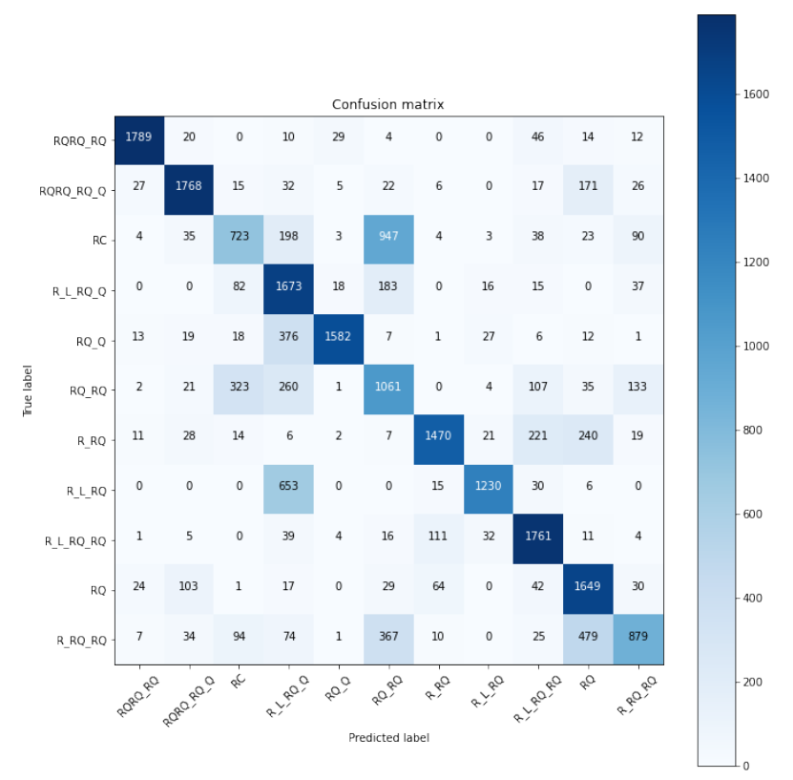
\includegraphics[width=0.9\textwidth]{Figuras/matriz de confusão do modelo treinado.png}
    \legend{Fonte: Imagem gerada pelo algoritmo de treinamento.}
    \label{figura20}
\end{figure}

A matriz é apresentada como um mapa de calor em tons de azul, em que a intensidade da cor é
proporcional ao número de amostras em cada combinação de classe verdadeira (linhas) e classe
predita (colunas). A diagonal principal concentra os maiores valores, confirmando que o
modelo acerta a classificação na grande maioria dos casos.
As topologias que apresentaram maior taxa de acerto absoluto foram:

\begin{itemize}
    \item RQRQ\_{RQ}: 1.789 acertos.
    \item RQRQ\_{RQ\_Q}: 1.768 acertos.
    \item R\_{L}\_RQ\_{RQ}: 1.761 acertos.
    \item R\_{L}\_RQ\_{Q}: 1.673 acertos.
    \item RQ: 1.649 acertos.
\end{itemize}

Por outro lado, as maiores confusões ocorreram entre topologias estruturalmente próximas. A
classe RQ apresentou 947 amostras classificadas incorretamente como RQ\_{RQ}, e a classe
R\_{L}\_RQ teve 653 amostrar confundidas como R\_{L}\_RQ\_{Q}. A classe R\_RQ\_{RQ} foi a que
apresentou o menor número de acertos absolutos (879), com 479 amostras sendo classificadas
como RQ, circuito com topologia semelhante, diferindo apenas pela ausência do ramo resistivo
em série. 

Esses padrões de confusão são fisicamente coerentes: topologias que compartilham
elementos de circuito ou que diferem apenas na presença de um componente adicional tendem
a gerar espectros de impedância com formas muito semelhantes, tornando sua distinção um
desafio inerente ao problema de classificação. Os resultados obtidos demonstram que a
combinação entre dados sintéticos fisicamente consistentes, normalização dos espectros
fundamentada na literatura e utilização de rede neurais convolucionais unidimensionais
constitui uma abordagem promissora para identificação automática de circuitos equivalentes
em EIS.

Embora a CNN tenha demonstrado resultados promissores, com \textit{F1-Score} de aproximadamente
$70,9\%$, o custo computacional e o tempo de treinamento elevados – decorrentes da necessidade
de ajustar milhares de parâmetros ao longo de até 3 mil épocas – tornaram necessária a
investigação de abordagem alternativas. Ademais, a complexidade de construção, configuração
e interpretação de uma CNN representa uma barreira prática em cenários que demandam soluções mais acessíveis e de menos custo computacional. 

Nesse contexto, a literatura recente
em IES aponta que algoritmos clássicos de aprendizado de máquina como florestas aleatórias
(\textit{Random forest} - RF) e métodos baseados em gradiente, têm apresentado resultados
competitivos na tarefa de identificação e classificação de circuitos equivalentes \cite{schaeffer2023machine}. Com base
nessa motivação, foram avaliados sistematicamente dez algoritmos distintos da biblioteca
\textit{scikit-learn}, além de \textit{XGBoost} e do LightGBM, utilizando a mesma base de dados e os mesmos
protocolos de divisão treino/teste empregados nos experimentos com a CNN.

Os dados utilizados foram os mesmos 110 mil EIS armazenados no MongoDB, distribuídos
entre as 11 topologias de circuito equivalente. Para este conjunto de experimentos, foi utilizada
a mesma função de normalização descrito anteriormente -- incluindo a normalização logarítmica
da frequência pela mediana -- e o vetor de atributos foi formado pela concatenação da frequência
normalizada com as partes real e imaginária da impedância normalizada, resultando em vetores
de dimensões $3 \times 181 = 543$ atributos por amostra.

Essa configuração é idêntica à utilizada
no treinamento da CNN, garantindo comparabilidade direta entre os resultados dos dois
conjuntos de experimentos. Os rótulos das classes foram codificados numericamente por meio
o \textit{LabelEncoder} do \textit{Scikit-learn}. Os dados foram divididos em 80\% para treinamento e 20\%
para teste (\textit{train\_test\_split} com \textit{Random\_state = 42}). Para cada modelo, além da acurácia sobre
o conjunto de treinamento, foi calculada a acurácia por validação cruzada estratificada com 10
folds (\textit{cross\_val\_predict}, \textit{cv = 10}), que fornece uma estimativa mais robusta da capacidade de
generalização do modelo. Os gráficos gerados para cada modelo seguem um padrão fixo de três
visualizações:

\begin{enumerate}
    \item Curva ROC (\textit{Receiver Operating Characteristic}) por classe, gerada com a
    biblioteca \textit{Yellowbrick}, exibindo a relação entre taxa de verdadeiros positivos e
    taxa de falsos positivos para cada uma das 11 topologias, com o valor de AUC
    (\textit{Area Under the Curve}) correspondente.

    \item Matriz Confusão (\textit{Confusion Matrix}), em formato de mapa de calor com a
    biblioteca \textit{Seaborn}, mostrando a distribuição das predições para cada par (classe
    verdadeiro, classe predita).

    \item \textit{Classification Report} visual, também gerado com \textit{Yellowbrick},
    exibindo as métricas de precisão, \textit{recall} e F1-score para classe individualmente.
\end{enumerate}

\section{\textit{Random Forest} (RF) - Floresta Aleatória}
 RF é um método de conjunto (ensemble) baseando na combinação de múltiplas árvores de
decisão treinadas sobre subamostras aleatórias dos dados e dos atributos. A predição final é
dada por votação majoritária entre as árvores, o que reduz a variância e aumenta a robustez do
classificador em relação a uma única árvore de decisão. O modelo foi treinando com os
parâmetros padrão do scikit-learn, chegando o valor da acurácia no treinamento de 99,54\% e o
acurácia por validação cruzada (10 folds) e 97,10\% e sem ajuste de hiperparâmetros. 

\begin{figure}[h]
    \centering
    \caption{Curva ROC por classe para o classificador RF. O AUC igual a 1,0 para
    todas as classes, exceto R\_{RQ} com AUC = 0,99, indicando excelente capacidade discriminativa
    do modelo.}
    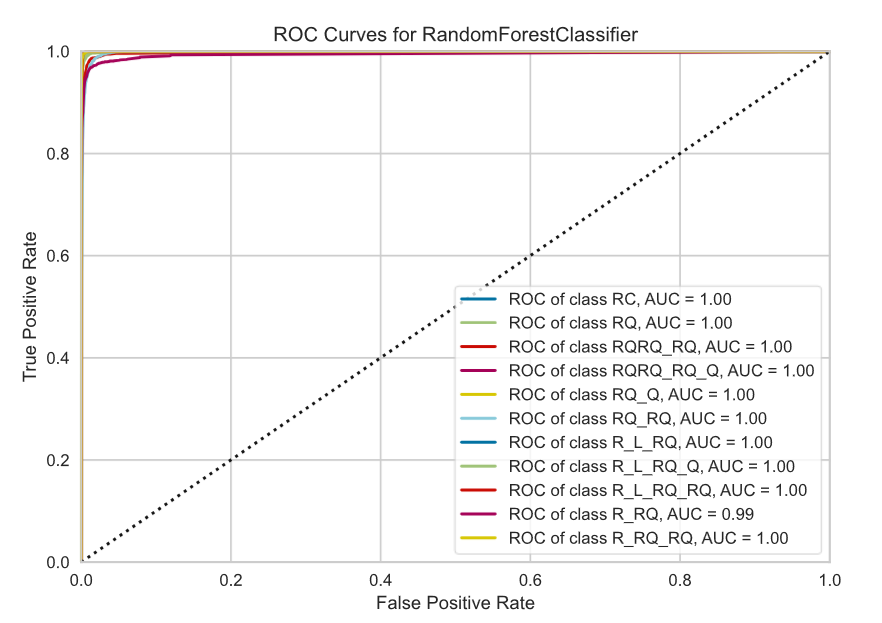
\includegraphics[width=0.9\textwidth]{Figuras/curva ROC por classe para o classificador RF.png}
    \legend{Fonte: Imagem gerada pelo script de treinamento.}
    \label{figura21}
\end{figure}

A curva ROC demonstra que o RF conseguiu separar praticamente todas as classes com
perfeição, com $AUC = 1{,}0$ para dez das onze topologias e $AUC = 0{,}99$ para a classe
R\_{RQ}, que historicamente apresenta maior confusão com classes estruturalmente
semelhantes. Os
resultados obtidos estão na Figura~\ref{figura21}.

\begin{figure}[h]
    \centering
    \caption{Matriz de confusão RF sobre o conjunto de teste. Os valores na diagonal
    principalmente indicam os acertos do modelo para cada topologia}
    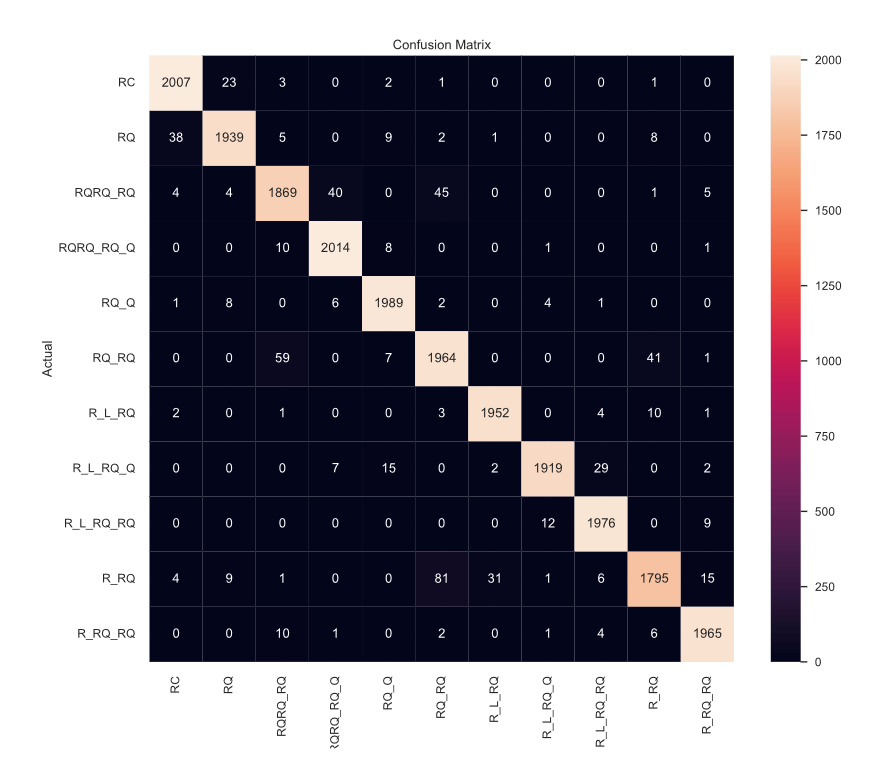
\includegraphics[width=0.9\textwidth]{Figuras/matriz de confusão RF.png}
    \legend{Fonte: Imagem gerada pelo script de treinamento.}
    \label{figura22}
\end{figure}
A matriz de confusão evidencia a alta concentração de acertos na diagonal principal, com poucos
erros distribuídos de forma esparsa. As maiores confusões ocorreram na classe RQ\_{RQ}, com
59 amostras classificadas como RQRQ\_{RQ}, e na classe R\_{RQ}, com 81 amostras classificadas
como RQ\_{RQ}, padrão coerente com a semelhança estrutural entre essas topologias, como ilustrado na Figura~\ref{figura22}.

O relatório de classificação confirma o alto desempenho do modelo: os valores de precisão,
\textit{recall} e \textit{F1-score} para cada classe ficaram entre 0,924 e 0,990, demonstrando desempenho
consistente e equilibrado em todas as topologias, como ilustrado na Figura~\ref{figura23}.


\begin{figure}[h]
    \centering
    \caption{Relatório de classificação do RF, com precisão, recall e F1Score por classe.}
    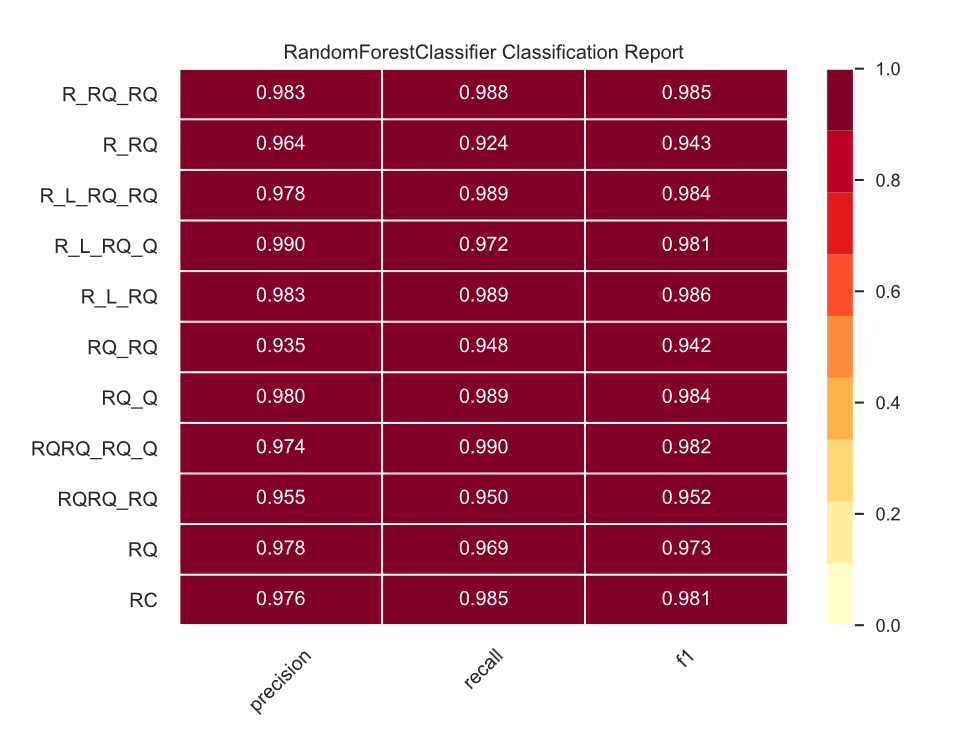
\includegraphics[width=0.8\textwidth]{Figuras/relatório de classificação do RF.png}
    \legend{Fonte: Imagem gerada pelo script de treinamento.}
    \label{figura23}
\end{figure}

\section{\textit{k-Nearest Neighbours} (KNN)}
KNN é um algoritmo de classificação baseado em similaridade para classificar um
novo espectro, o algoritmo identifica os $k$ vizinhos mais próximos no espaço de atributos
(usando distância euclidiana por padrão) e atribui a classe mais frequente entre eles. Trata-se
de um algoritmo não paramétrico, sem fase explícita de treinamento, mas com custo de predição
proporcional ao tamanho do conjunto de dados. Em espaços de alta dimensionalidade, o KNN
tende a sofrer com o fenômeno conhecido como \textit{curse of dimensionality} (maldição da
dimensionalidade), em que as distâncias euclianas perdem capacidade discriminativa à medida que a dimensão aumenta. O modelo foi treinado com os parâmetros padrões chegando ao o
valor de acurácia no treinamento de 92,73\% e a acurácia por validação cruzada (10 folds) de
88,93\% e se usar qualquer tipo de hiperparâmetros.

\begin{figure}[htbp]
    \centering
    \caption{Curvas ROC por classe para o KNN. Os menores AUCs foram registrados
    para R\_{RQ} (AUC = 0,95), RQ (AUC = 0,98) e RQRQ\_{RQ} (AUC = 0,98),
    refletindo maior dificuldade de separação nessas classes.}
    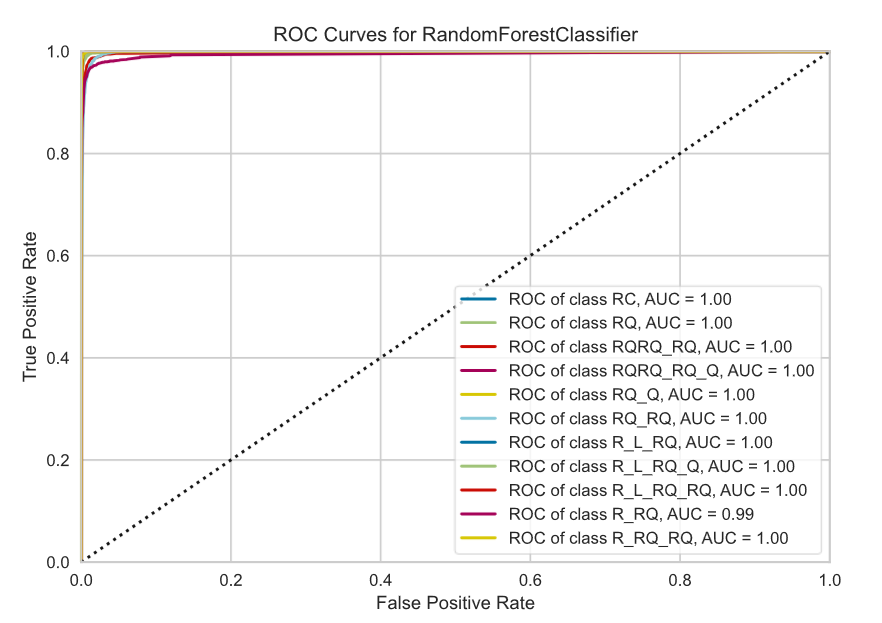
\includegraphics[width=0.9\textwidth]{Figuras/curva ROC por classe para o classificador RF.png}
    \legend{Fonte: Imagem gerada pelo script de treinamento.}
    \label{figura24}
\end{figure}

A curva ROC do KNN mostra desempenho inferior ao RF, com AUC entre 0,95 e
1,0. As classes R\_{RQ} (AUC = 0,95) e RQ (AUC = 0,98) apresentaram maior dificuldade de
separação, enquanto R\_{L\_RQ\_{RQ}} e R\_{RQ\_{RQ}} atingiram AUC = 1,0, como ilustrado na Figura~\ref{figura24}.

\begin{figure}[htbp]
    \centering
    \caption{Matriz de confusão do KNN sobre o conjunto de teste. A classe R\_{RQ}
    apresentou o maior número de erros absolutos, com 209 amostras classificadas incorretamente
    como R\_{RQ}.}
    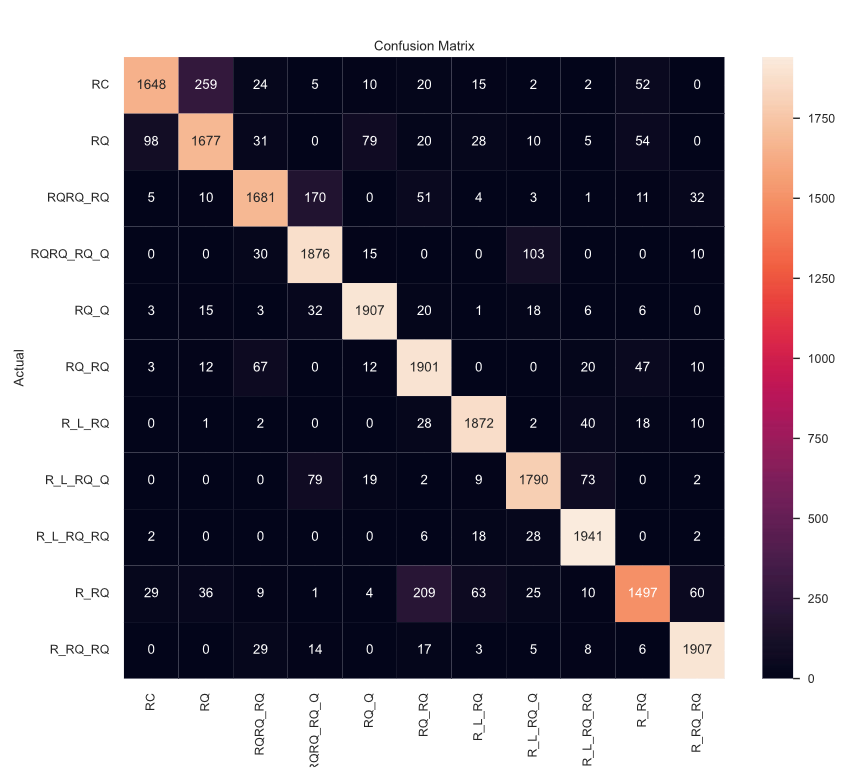
\includegraphics[width=0.9\textwidth]{Figuras/matriz de confusão do KNN sobre o conjunto de teste.png}
    \legend{Fonte: Imagem gerada pelo script de treinamento.}
    \label{figura25}
\end{figure}

A matriz de confusão revela que a classe R\_{RQ} foi a mais prejudicada: 209 amostras
foram classificadas como RQ\_{RQ} e 63 como R\_{L\_RQ}, totalizando 436 erros -- o pior
desempenho absoluto entre todas as classes e modelos avaliados, como ilustrado na Figura~\ref{figura25}. A classe RC também
apresentou número elevado de erros (389 amostras mal classificadas), especialmente confundida como RQ (259 erros). Isso reflete a dificuldade do KNN de separar classes cujos
espectros diferem em escala ou forma de maneira não linear, como ilustrado na Figura~\ref{figura26}.

\begin{figure}[htbp]
    \centering
    \caption{Relatório de classificação do KNN. O menor F1-score foi observado na
    classe R\_{RQ} (0,824), e os maiores em R\_{L\_RQ\_RQ} (0,946) e R\_{RQ} (0,948).}
    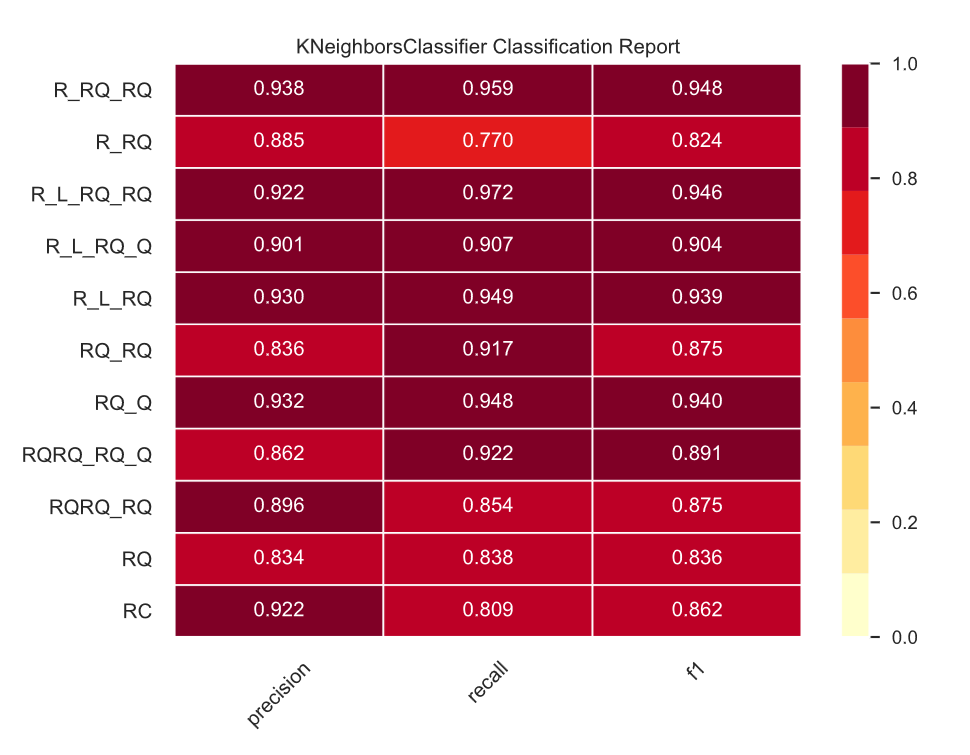
\includegraphics[width=0.9\textwidth]{Figuras/relatório de classificação do KNN.png}
    \legend{Fonte: Imagem gerada pelo script de treinamento.}
    \label{figura26}
\end{figure}

As melhores topologia R\_L\_RQ\_RQ (F1 0.946), R\_RQ\_RQ (F1 0.948) e R\_L\_RQ
(F1 0.939) e os piores topologia R\_RQ (precisão 0,885, recall 0,77; F1 0,824) e RQ\_RQ (F1
0,875), evidenciando que topologias com elementos resistivos isolados são mais difíceis para o KNN.

\section{Árvore de Decisão}
A árvore de decisão é um modelo que particiona o espaço de atributo por meio de
regra binárias sucessivas aprendidas a partir dos dados de treinamento, formando uma estrutura
hierárquica. Cada nó interno representa uma condição sobre um atributo, e cada folha representa
uma classe predita. Sem poda, uma árvore de decisão pode crescer até memorizar complemente
o conjunto de treinamento, o que explica a alta acurácia de treino, mas o desempenho
ligeiramente inferior na validação cruzada em comparação ao RF. O modelo foi treinado com
os parâmetros padrões da biblioteca, chega na acurácia no treinamento de 99,54\% e acurácia
por validação cruzada (10 folds) 95,85\%.

\begin{figure}[htbp]
    \centering
    \caption{Curva ROC da árvore de decisão. Os menores AUCs foram observados
    em R\_{RQ} (AUC = 0,95), RQ (AUC = 0,97), RQRQ\_{RQ} (AUC = 0,97) e
    RQ\_{RQ} (AUC = 0,97).}
    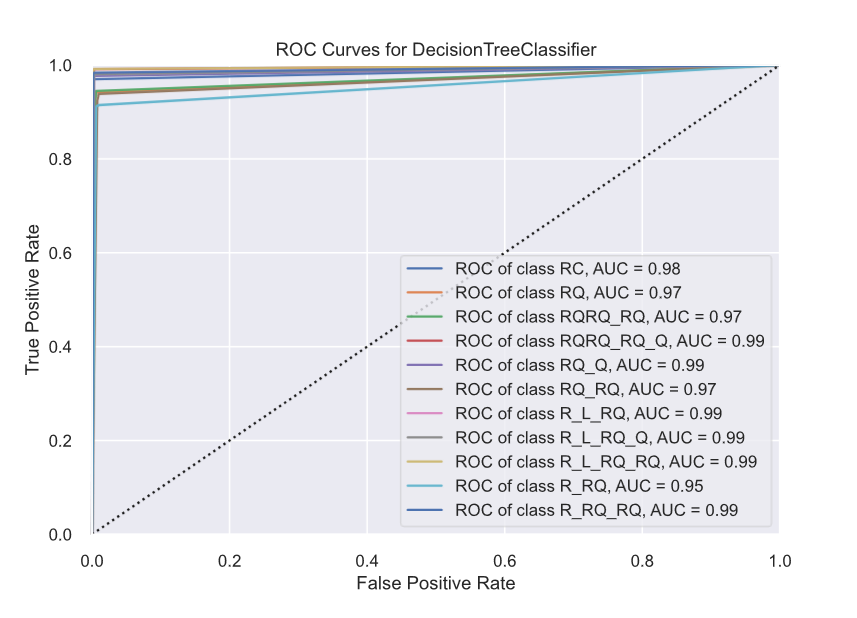
\includegraphics[width=0.9\textwidth]{Figuras/curva ROC da árvore de decisão.png}
    \legend{Fonte: Imagem gerada pelo script de treinamento.}
    \label{figura27}
\end{figure}

A curva ROC da árvore de decisão mostra AUC entre 0.95 e 0.99 para maioria das
classes, com R\_RQ novamente apresentando o menor valor (AUC=0.95). Comparando com o KNN, os AUCs são semelhantes, mas o arvore de decisão mostrou padrão de erros diferente na matriz de confusão, como ilustrado na Figura~\ref{figura27}.

\begin{figure}[htbp]
    \centering
    \caption{Matriz de confusão da árvore de decisão sobre o conjunto de teste. A classe R\_RQ apresentou 171 erros, com maior confusão com RQ\_RQ (77 amostras) e R\_L\_RQ (35 amostras).}
    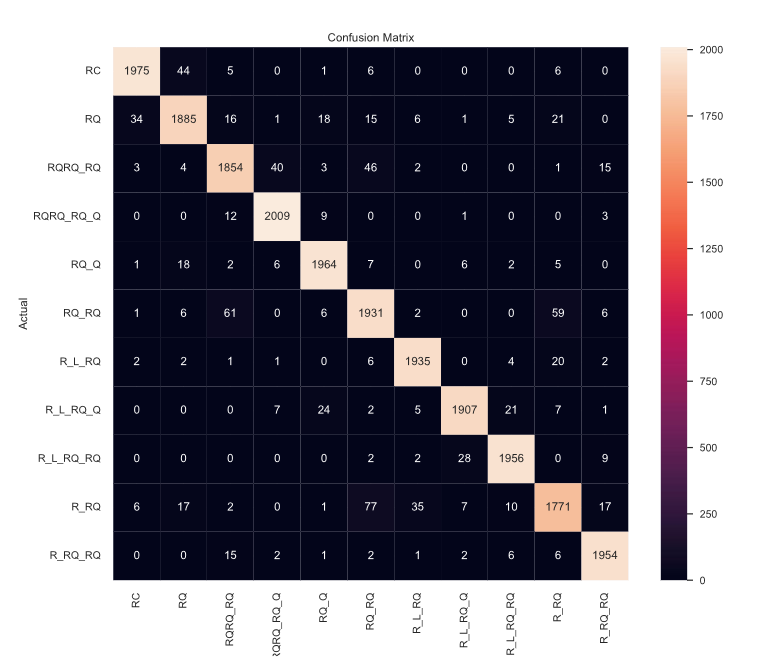
\includegraphics[width=0.9\textwidth]{Figuras/matriz de confusão da árvore de decisão sobre o conjunto de teste.png}
    \legend{Fonte: Imagem gerada pelo script de treinamento.}
    \label{figura28}
\end{figure}

A matriz de confusão da Árvore de decisão apresentou padrão de similar ao RF, porém com erros mais distribuídos. A classe R\_RQ continuou sendo a mais problemática (171 erros totais). RQRQ\_RQ também apresentou erros relevantes: 46 amostras classificadas como
RQ\_RQ e 40 como RQRQ\_RQ\_Q. O comportamento reflete o sobreajustes característico de árvore sem poda, que constroem fronteiras de decisão excessivamente específicas ao treinamento, como ilustrado na Figura~\ref{figura28}.

\begin{figure}[htbp]
    \centering
    \caption{Relatório de classificação da árvore de decisão. Os menores F1-score
    foram registrados em R\_RQ (0.923) e RQ\_RQ (0.927), enquanto RQRQ\_RQ\_Q ( F1 0.980) e
    R\_L\_RQ\_RQ (f1 0.978) obtiveram os melhores resultados.}
    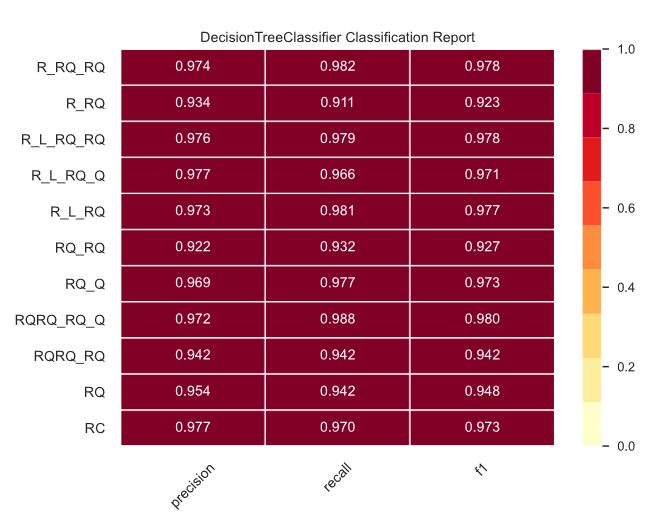
\includegraphics[width=0.9\textwidth]{Figuras/relatório de classificação da árvore de decisão.png}
    \legend{Fonte: Imagem gerada pelo script de treinamento.}
    \label{figura29}
\end{figure}

Melhores topologias RQRQ\_RQ\_Q (F1 0.980), RC (F1 0.973), RQ\_Q (F1 0.973)
e R\_L\_RQ\_RQ (F1 0.978). Pior topologias R\_RQ (F1 0.923) e RQ\_RQ (F1 0.927) – mesmo
padrão observado no RF, confirmando que essas topologias são intrinsecamente mais difíceis
de classificar,  como ilustrado na Figura~\ref{figura29}.


\section{Regressão Logística}
A regressão logística é um classificador linear que estima a probabilidade de
pertencimento a cada classe por meio de uma combinação linear dos atributos, transformada
pela função sigmoide (ou \textit{softmax}, no caso multiclasse). Apesar do nome regressão, trata-se de
um algoritmo de classificação. Sua limitação fundamental é a suposição de separabilidade
linear: o modelo só consegue aprender fronteiras de decisão lineares no espaço de atributos. O
modelo foi configurado com \textit{LogisticRegression}(\textit{solver} = \texttt{'lbfgs'},
\textit{max\_iter} = 1000).

Durante o treinamento, o otimizador não conseguiu convergir dentro do número máximo de
iterações, indicando que os dados não são linearmente separáveis nesta representação. Os
resultados foram acurácia no treino de 9,05\%, acurácia por validação cruzada (10 folds) de
9,05\% e tempo de treinamento de aproximadamente 41 segundos.

\begin{figure}[htbp]
    \centering
    \caption{ Matriz de confusão a), relatório de classificação b) e curva ROC c) de regressão logística. O desempenho próximo ao aceso de (~9.09\% para 11 classes) indica que os espectros não são linearmente separáveis no espaço de atributos utilizado.}
    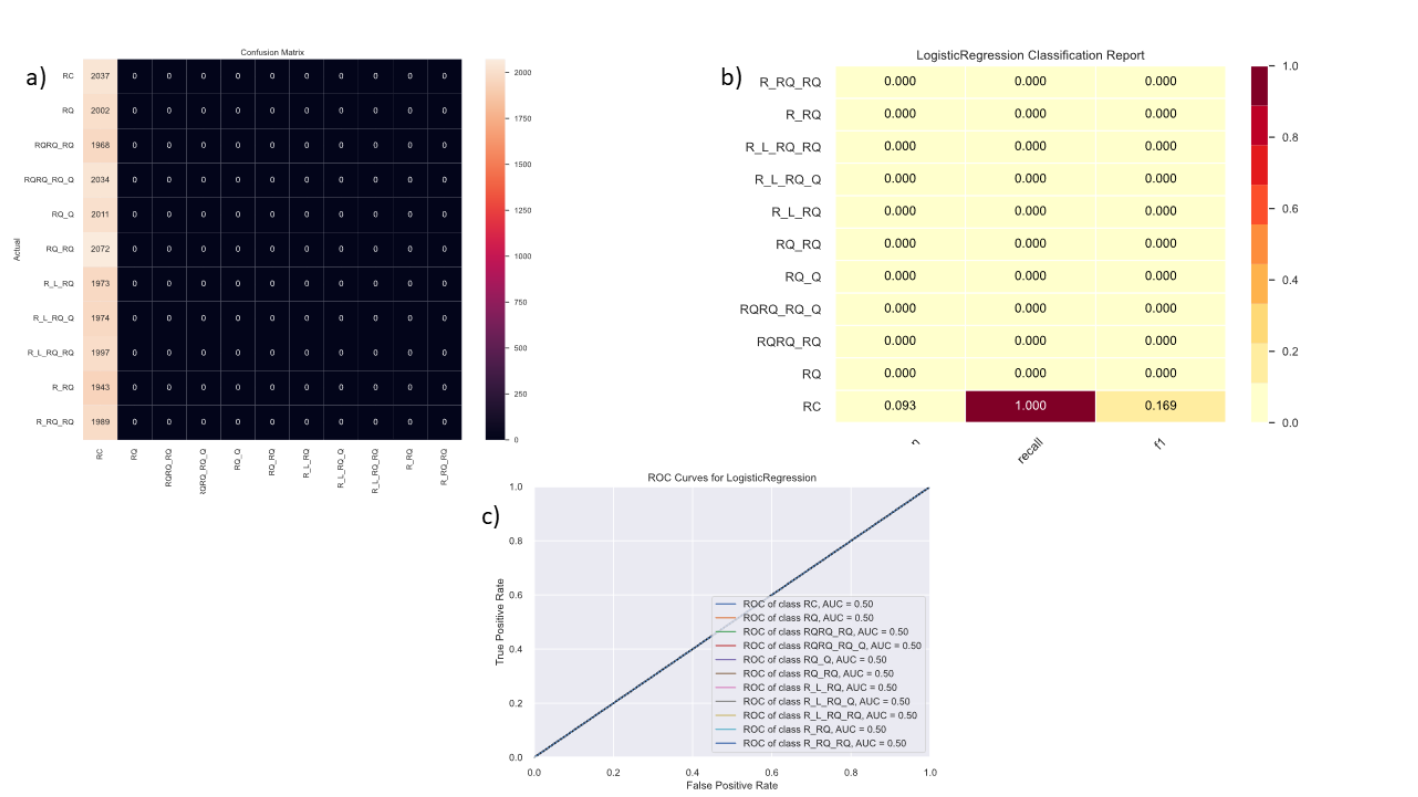
\includegraphics[width=0.9\textwidth]{Figuras/matriz de confusão a), relatório de classificação b) e curva ROC c) de regressão logística..png}
    \legend{Fonte: Imagem gerada pelo script de treinamento.}
    \label{figura30}
\end{figure}

O desempenho da regressão logística foi essencialmente igual ao de um
classificador aleatório: para um problema de 11 classes equiprováveis, a acurácia esperada ao
acesso é 1/11 $\approx$ 9.09\% , e o modelo atingiu exatamente 9.05\%. Esse resultado confirma que
as relações entre os atributos dos espectros e as classes de circuito equivalente são
intrinsecamente não lineares, inviabilizando o uso de classificadores lineares para este
problema, como ilustrado na Figura~\ref{figura30}.


\section{\textit{Gaussian Naive Bayes}}
O \textit{Gaussian Naive Bayes} ou \textit{Naive Bayes} é um classificador probabilístico baseado
no Teorema de Bayes com a suposição ingênua (naive) de independência condicional entre os
atributos como uma distribuição gaussiana, estimando média e variância por classe a partir dos dados de treinamento. Apesar de sua simplicidade, é computacionalmente muito eficiente e
funciona bem em dados de alta dimensionalidade quando a suposição de independência é
aproximadamente válida. Os resultados foram da acurácia no treino de 15,85\%, acurácia por
validação cruzada (10 folds) 15,86\% e o tempo de treinamento foi de aproximadamente de 39
segundos.
\begin{figure}[htbp]
    \centering
    \caption{Matriz de confusão d), relatório de classificação e) e curva ROC f) do
    gaussian Naive Bayess. O desempenho ligeiramente acima do acaso (15.85\%) indica suposição
    de independência antre atributos é fortemente violada nos EIS. }
    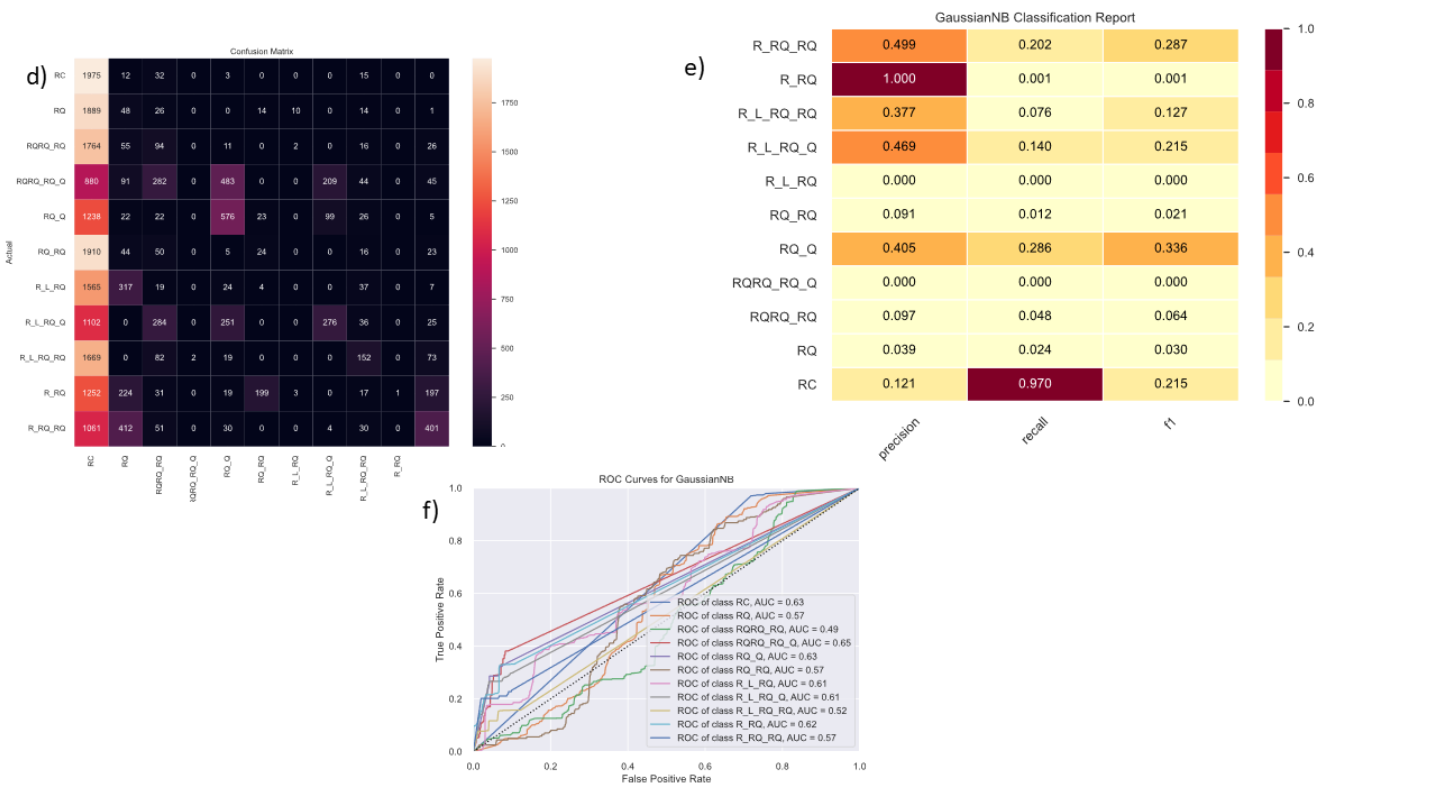
\includegraphics[width=0.9\textwidth]{Figuras/matriz de confusão d), relatório de classificação e) e curva ROC f) do gaussian Naive Bayess.png}
    \legend{Fonte: Imagem gerada pelo script de treinamento.}
    \label{figura31}
\end{figure}

O Naive Bayes atingiu 15,85\% de acurácia, ligeiramente superior ao acaso, mas
muito abaixo dos modelos baseados em árvores. O baixo desempenho é esperado nos EIS, as
partes real e imaginária são fisicamente acoplados e correlacionadas ao longo do eixo de
frequência. A suposição de independência condicional viola diretamente essa estrutura,
impedindo que o modelo capture os padrões relevantes, como ilustrado na Figura ~\ref{figura31}. 

\section{\textit{Linear Support Vector Machine} (LinearSVC) ou SVM}
O SVM busca o hiperplano de separação de máximo margem entre as classes no
espaço de atributos. A versão \textit{linear LinearSVC} é computacionalmente mais eficiente que as
versões com o kernel, adequada para grandes volumes de dados. Assim como Regressão
logística, o SVM pressupõe separabilidade linear, o que representa uma limitação fundamental
para este problema. Os resultados foram de acurácia no treino de 20,91\%, acurácia por
validação cruzada (10 folds) de 17,64\% e o tempo de treinamento foi de aproximadamente 5
horas e 54 minutos.
\begin{figure}[htbp]
    \centering
    \caption{Matrix de confusão g), relatório de classificação h) e a curva ROC i) do SVM. Além do baixo desempenho (20.91\%), o modelo demandou aproximadamente de 5 horas e 54 minutos de treinamento, tornando-o inviável para este problema.}
    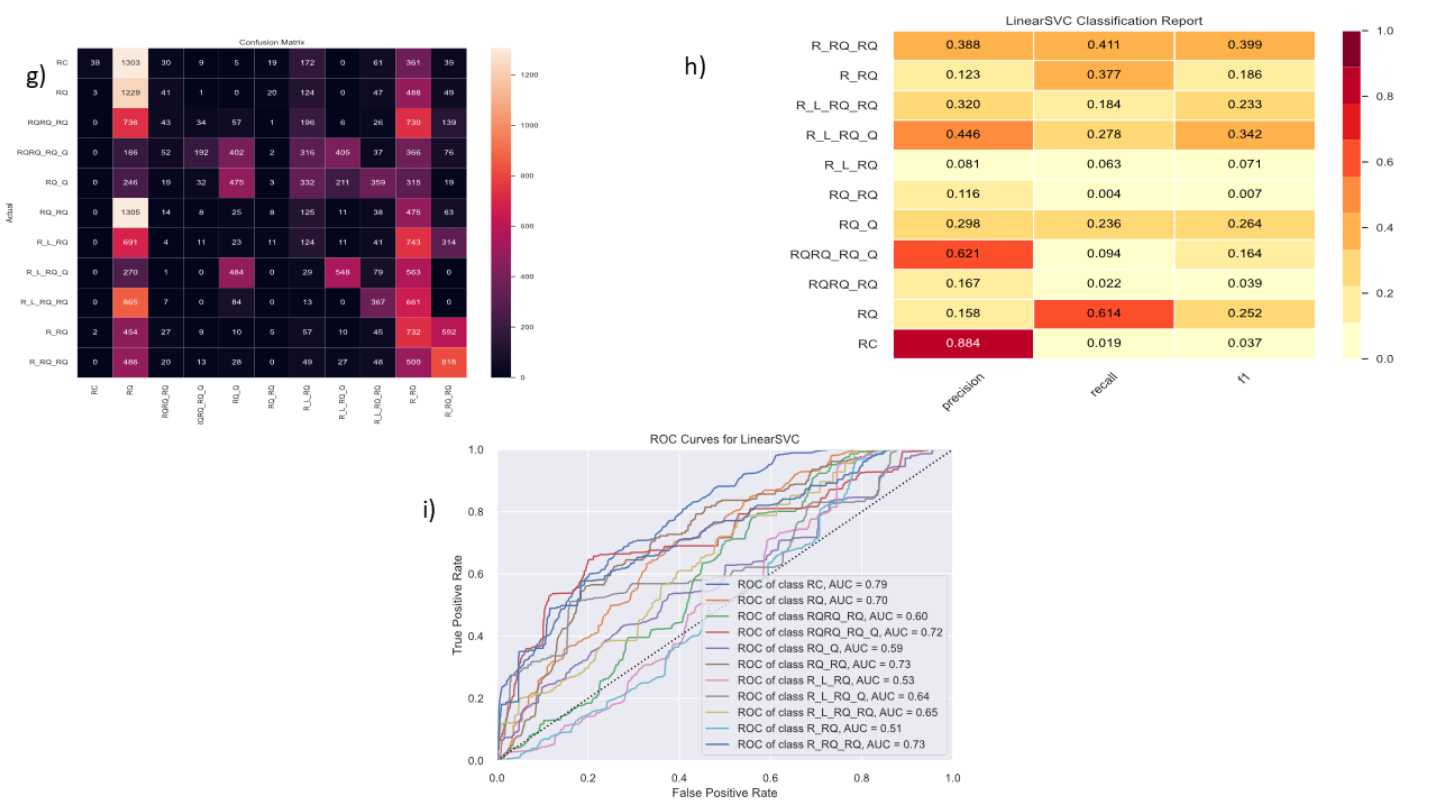
\includegraphics[width=0.9\textwidth]{Figuras/matrix de confusão g), relatório de classificação h) e a curva ROC i) do SVM.png}
    \legend{Fonte: Imagem gerada pelo script de treinamento.}
    \label{figura32}
\end{figure}

O SVM apresentou desempenho franco (20.9\%) combinado com tempo de treinamento
muito grande (~5h 54 min), resultado da dificuldade do algoritmo de encontrar hiperplanos
separadores válidos em dados não linearmente separáveis com 543 atributos. Esses resultados, somados aos da regressão logística consolidam a conclusão de que modelos lineares são
inadequados para a classificação de espectros de impedância, como ilustrado na Figura~\ref{figura32}.

\section{XGBoost (\textit{Extreme Gradient Boosting} - XGB)}
O XGB é um algoritmo de conjunto baseado em boosting de árvores de decisão,
que combina sequencialmente modelos fracos minimizando uma função de perda por meio de
descida de gradiente. A cada iteração uma nova árvore é treinada para corrigir os erros residuais
da iteração anterior. O XGB inclui regularidade L1 e L2, tratamento nativo de valores ausente
e otimizações de paralelização que o tornam significativamente mais eficiente que o Gradiente
Boosting nativo da scikit-learn. Os resultados foram de acurácia no treino de de 98,15\%, acurácia por validação cruzada (10 folds): 96,81\% e tempo de treinamento de aproximadamente
56 minutos e 13 segundos.

\begin{figure}[htbp]
    \centering
    \caption{Curva ROC por classe para XGB AUC=1.0 para todas as 11 topologias, indicando capacidade discriminativa perfeita do modelo no espaço de pontuações.}
    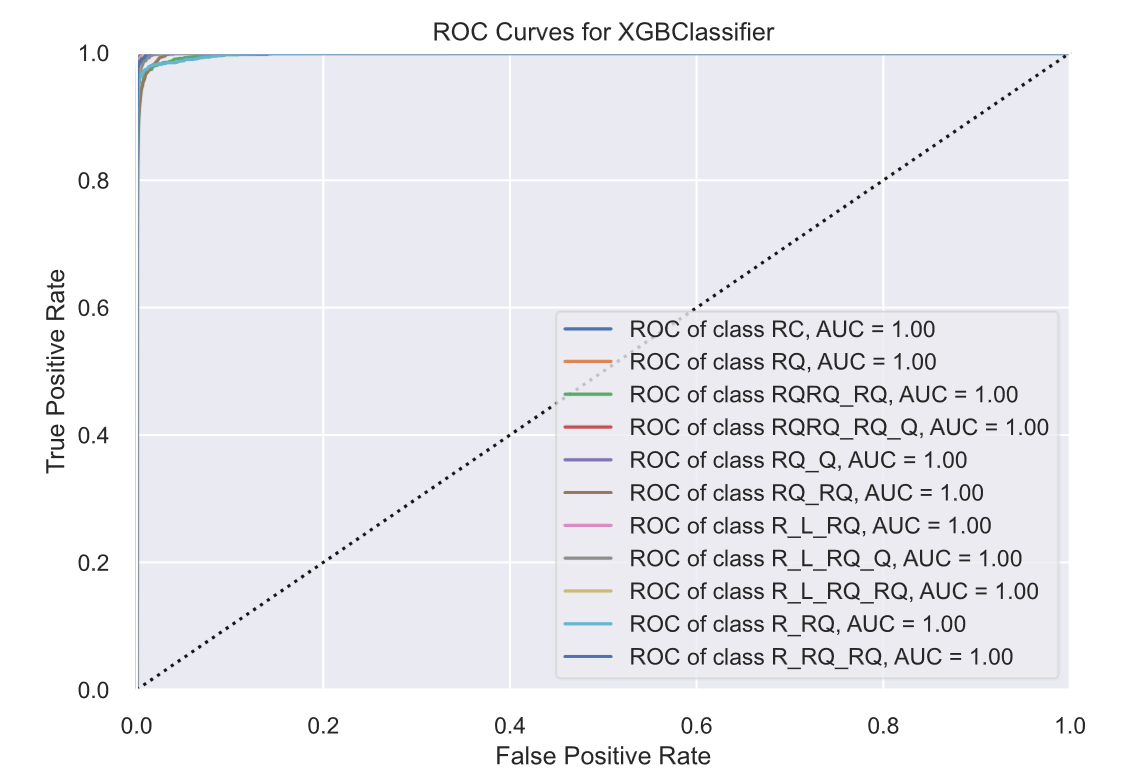
\includegraphics[width=0.9\textwidth]{Figuras/curva ROC por classe para XGB AUC=1.0 para todas as 11 topologias.png}
    \legend{Fonte: Imagem gerada pelo script de treinamento.}
    \label{figura33}
\end{figure}
 
A curva ROC da XGB atingiu AUC = 1.0 para todas as 11 classes – resultados superiores ao RF, que registrado AUC=0.99 para R\_RQ. Isso indica que o XGB separa perfeitamente as classes em termos de pontuação de probabilidade, mesmo que alguns erros ainda ocorram na
predição final (classe predita), como ilustrado na Figura~\ref{figura33}.

\begin{figure}[htbp]
    \centering
    \caption{Matriz de confusão do XGB sobre o conjunto de teste. As maiores
    confusões ocorreram entre RQRQ\_{RQ} e RQRQ\_{Q} (59 amostras) e entre RQ\_{RQ}.}
    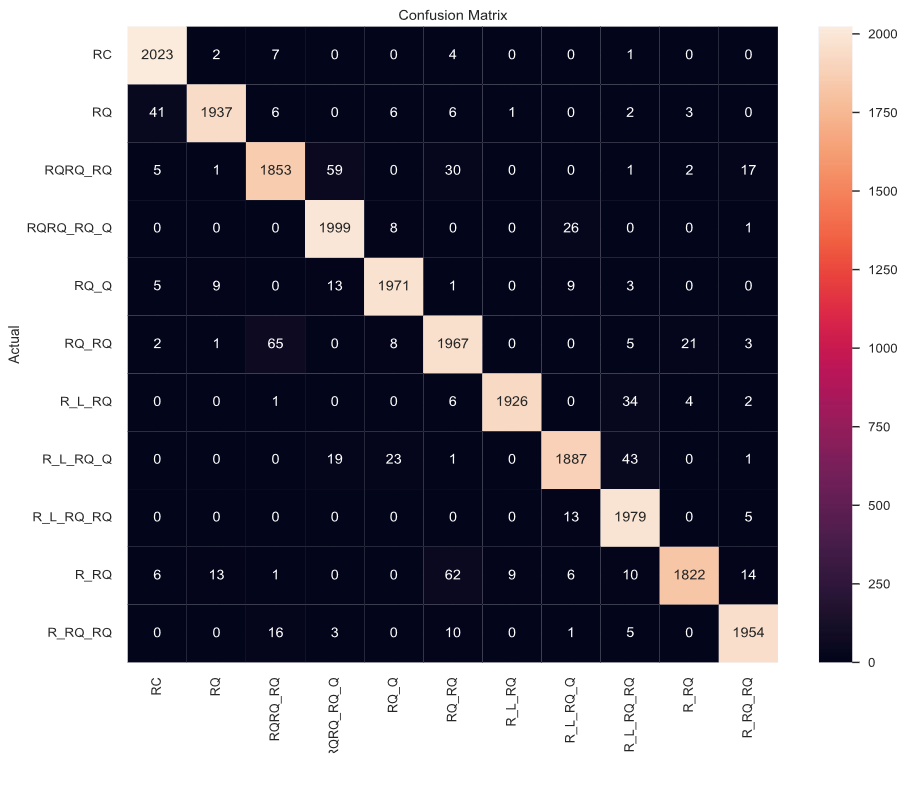
\includegraphics[width=0.9\textwidth]{Figuras/matriz de confusão do XGB sobre o conjunto de teste.png}
    \legend{Fonte: Imagem gerada pelo script de treinamento.}
    \label{figura34}
\end{figure}

A matriz de confusão do XGB apresenta erros menos numerosos e mais concentrados que os
observados no KNN e na árvore de decisão. As principais confusões ocorreram entre
RQRQ\_{RQ} e RQRQ\_{RQ\_Q} (59 erros), entre RQ\_{RQ} e RQRQ\_{RQ} (65 erros),
e entre R\_{RQ} e RQ{RQ} (62 erros). O padrão é consistente com os outros modelos, reforçando que essas confusões refletem a semelhança física entre as
topologias e não limitações do algoritmo, como ilustrado na Figura~\ref{figura34}.

\begin{figure}[htbp]
    \centering
    \caption{Relatório de classificação do XGB. Os melhores resultados foram
    obtidos em R\_{L\_RQ} (precisão 0,995; F1-score 0,985) e RC (recall 0,993;
    F1-score 0,982). Os menores F1-scores foram registrados em RQ\_{RQ} (0,946)
    e RQRQ\_{RQ} (0,946).}
    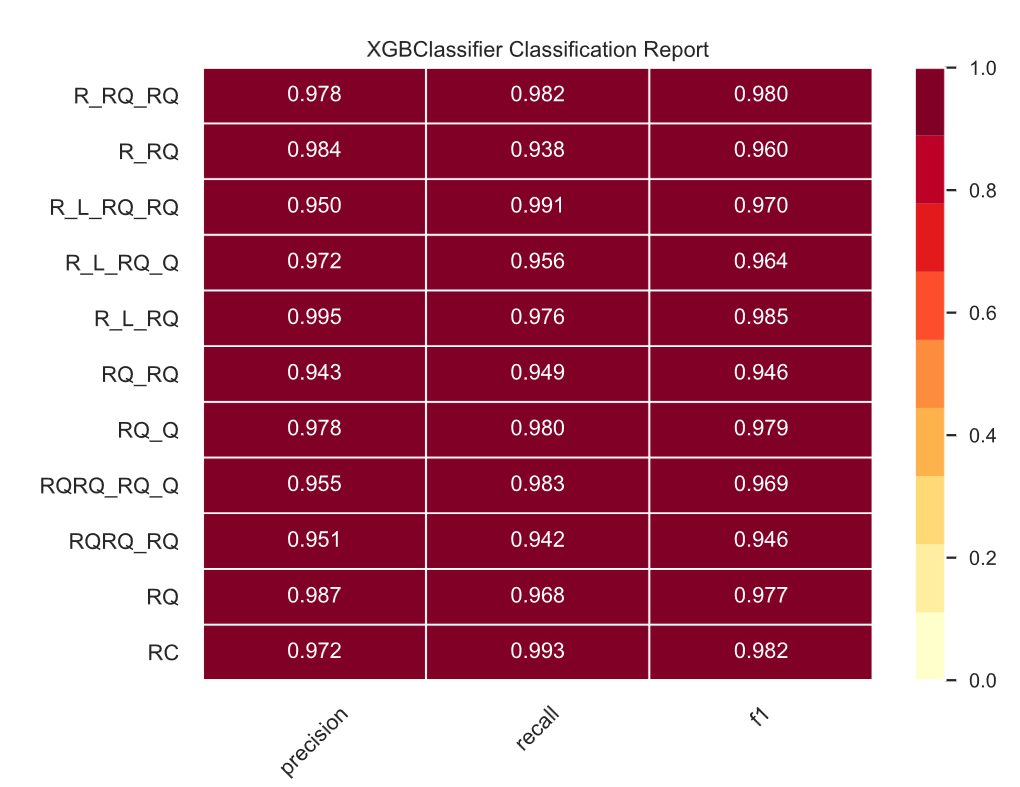
\includegraphics[width=0.9\textwidth]{Figuras/relatório de classificação do XGB.png}
    \legend{Fonte: Imagem gerada pelo script de treinamento.}
    \label{figura35}
\end{figure}

As melhores topologias foram R\_{L\_RQ} (precisão 0,995; F1-score 0,985), RC
(recall 0,993; F1-score 0,982) e RQ\_{Q} (F1-score 0,979), enquanto as piores
topologias foram RQ\_{RQ} (F1-score 0,946) e RQRQ\_{RQ} (F1-score 0,946), ambas
com confusões recíprocas elevadas. A topologia R\_{RQ} também apresentou desempenho
relativamente inferior (recall 0,938; F1-score 0,960), como ilustrado na Figura~\ref{figura35}.

\section{\textit{Gradiente Boosting} (GB)}
O Gradient Boosting nativo do scikit-learn é conceitualmente idêntico ao XGB na
abordagem de combinação sequencial de árvore rasas por descida de gradiente, porém sem as otimizações de paralelização e regularização presentes no XGB. Essa diferença de
implementação resulta em tempo de treinamento muito superior para grande volume de dados,
sem ganho proporcional de desempenho. Os resultados foram acurácia no treino 86.29\%,
acurácia por validação cruzada (10 folds): 85.34\% e tempo de treinamento foi de
aproximadamente 1 dia, 13 horas e 16 minutos.

\begin{figure}[htbp]
    \centering
    \caption{Matrix de confusão j), relatório de classificação k) e curva ROC l) do
    GB. O modelo apresentou acurácia de 86.29\% com tempo de treinamento superior a 37 horas
    confirmando sua inviabilidade prática frente ao XGB e ao LightGBM.}
    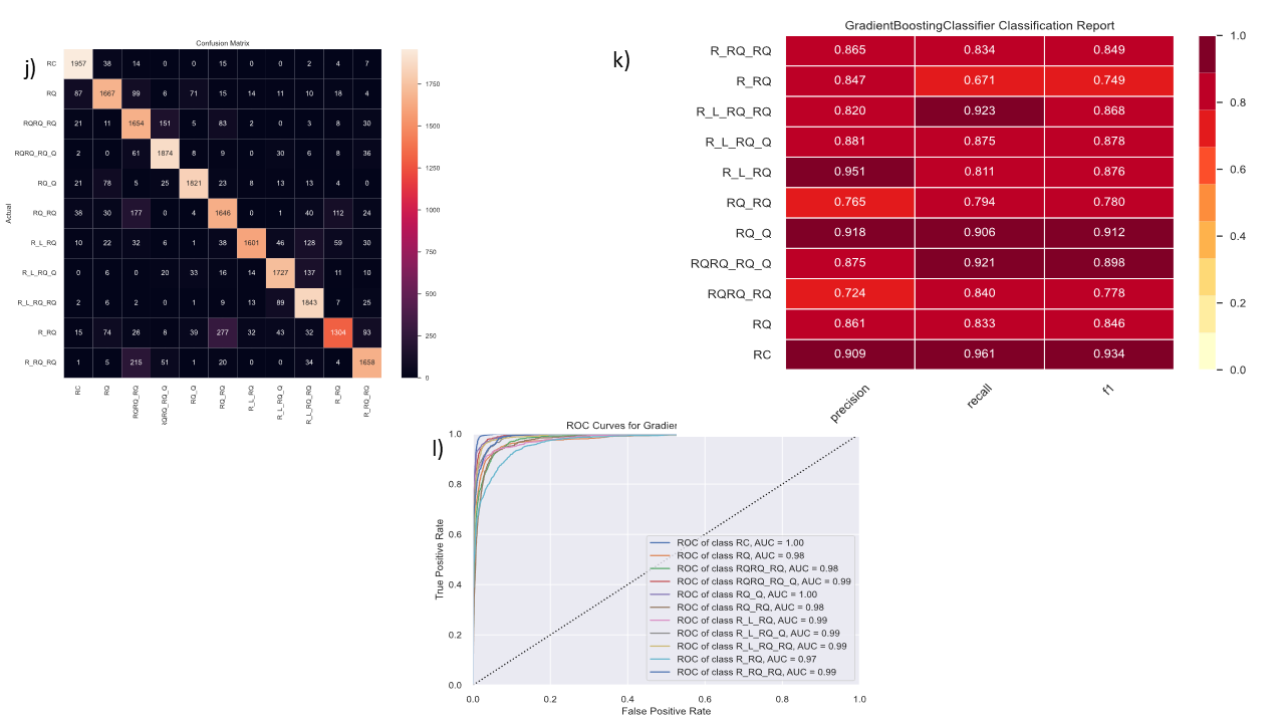
\includegraphics[width=0.9\textwidth]{Figuras/matrix de confusão j), relatório de classificação k) e curva ROC l) do GB.png}
    \legend{Fonte: Imagem gerada pelo script de treinamento.}
    \label{figura36}
\end{figure}

O GB apresentou desempenho inferior ao XGB (86.29\% vs. 98.15\%) com custo computacional
proibitivo – mais de 37 horas de treinamento contra 56 minutos do XGB. Esse resultado
evidencia que, para este volume de dados (110 mil) amostras com 543 atributos), a
implementação nativa do scikit-learn não é adequada, e as versões otimizadas (XGB e
LightGBM) devem ser preferidas, como ilustrado na Figura~\ref{figura36}. 

\section{\textit{Stochastic Gradient Descent} (SGDClassifier)}
O SGD implementa modelos lineares treinados com descida de gradiente
estocástico. A função de perda padrão (hinge) equivale a um SVM linear treinado de forma
estocástica, processando um exemplo por cez em vez do conjunto completo. Embora seja
muito eficiente computacionalmente, compartilha a limitação fundamental dos demais modelos
lineares: incapacidade de aprender fronteiras de decisão não lineares. Os resultados acurácia no
treino de 17,15\%, acurácia por validação cruzada (10 folds): 16,96\% e o tempo de treinamento
de 7 minutos e 1 segundo.

\begin{figure}[htbp]
    \centering
    \caption{Matriz de confusão m), relatório de classificação n) e curva ROC o) do
    SGD. Com acurácia de 17,15\%, o modelo confirmou o padrão observado nos demais
    classificadores lineares. Incapacidade de aprender fronteiras de decisão não lineares nos EIS.}
    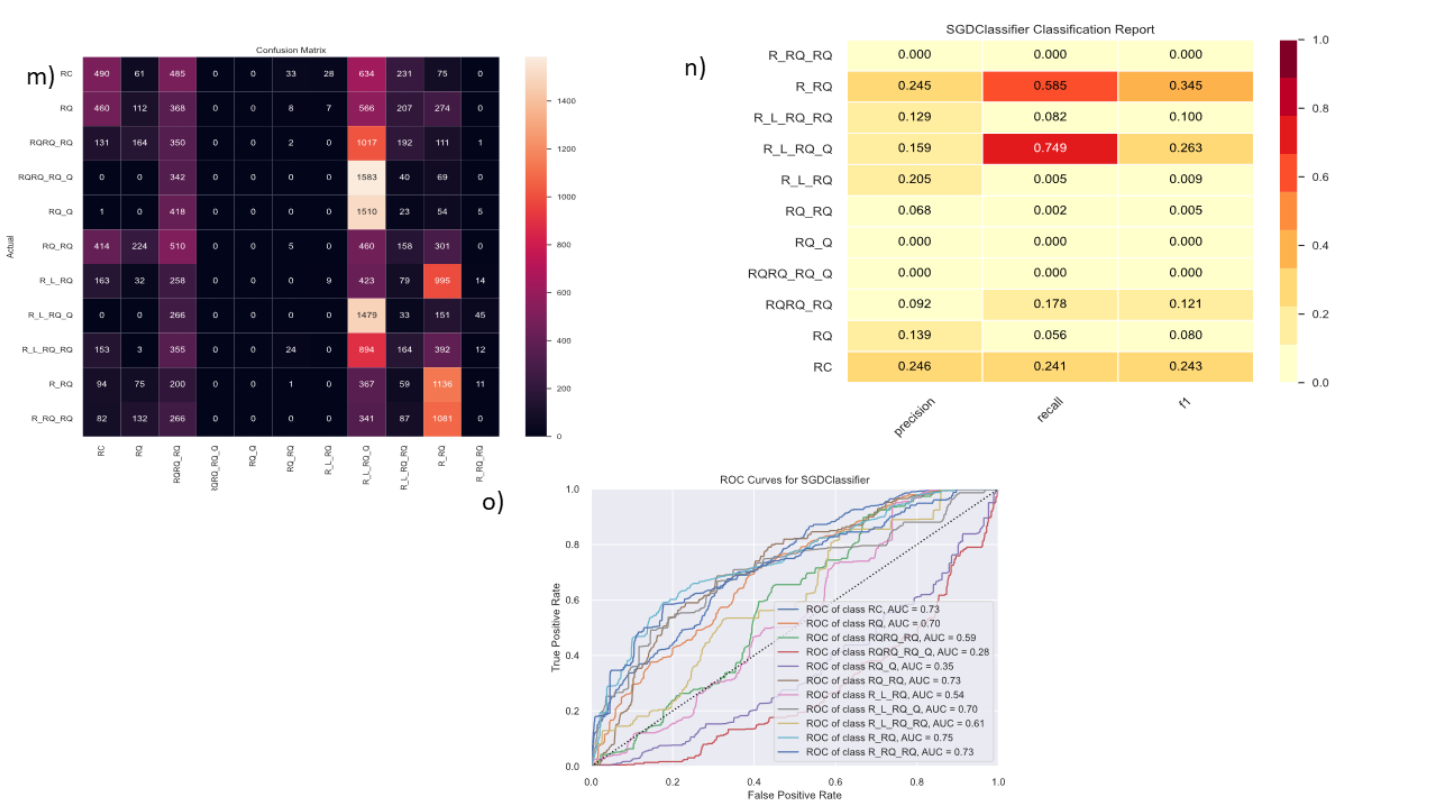
\includegraphics[width=0.9\textwidth]{Figuras/matriz de confusão m), relatório de classificação n) e curva ROC o) do SGD.png}
    \legend{Fonte: Imagem gerada pelo script de treinamento.}
    \label{figura37}
\end{figure}

O SGD reproduziu o baixo desempenho dos demais modelos lineares (17,15\%), em
linha com a Regressão Logística (9,05\%) e o SVM (20,91\%). A varação entre eles se deve
apenas às diferenças de implementação e estratégia de otimização, não a canho realiza de
capacidade preditiva sobre dados não linearmente separáveis, como ilustrado na Figura~\ref{figura37}.

\section{LightGBM (\textit{Light Gradient Boosting Machine} - LGBM)}
O LGBM é uma implementação altamente otimizada de gradiente boosting
desenvolvida pela Microsoft, com foco em eficiência computacional e baixo consumo de
memória. Diferencia-se do XGBoost e do \textit{gradient boosting} tradicional pelo uso de crescimento
de árvore por folha (\textit{leaf-wise}), em contraste com o crescimento por nível (\textit{level-wise}): em vez
de expandir todos os nós de um mesmo nível antes avançar, o LGBM seleciona a folha que
proporciona a maior redução de perda e a expande, independentemente do nível. Isso permite
que o modelo construa árvores mais assimétricas e profundas com menos iterações, geralmente
alcançando maior precisão com menor tempo de treinamento. Os resultados foram a acurácia no treino de 98,74\%, acurácia por validação cruzada (10 folds) 97,54\% e o tempo de
treinamento aproximadamente 21 minutos e 20 segundos. 
\begin{figure}[htbp]
    \centering
    \caption{Curva ROC por classe para o LGBM. AUC = 1.0 para todos as 11
    topologias, resultado idêntico ao XGB, confirmando a capacidade discriminativa perfeita do
    modelo.}
    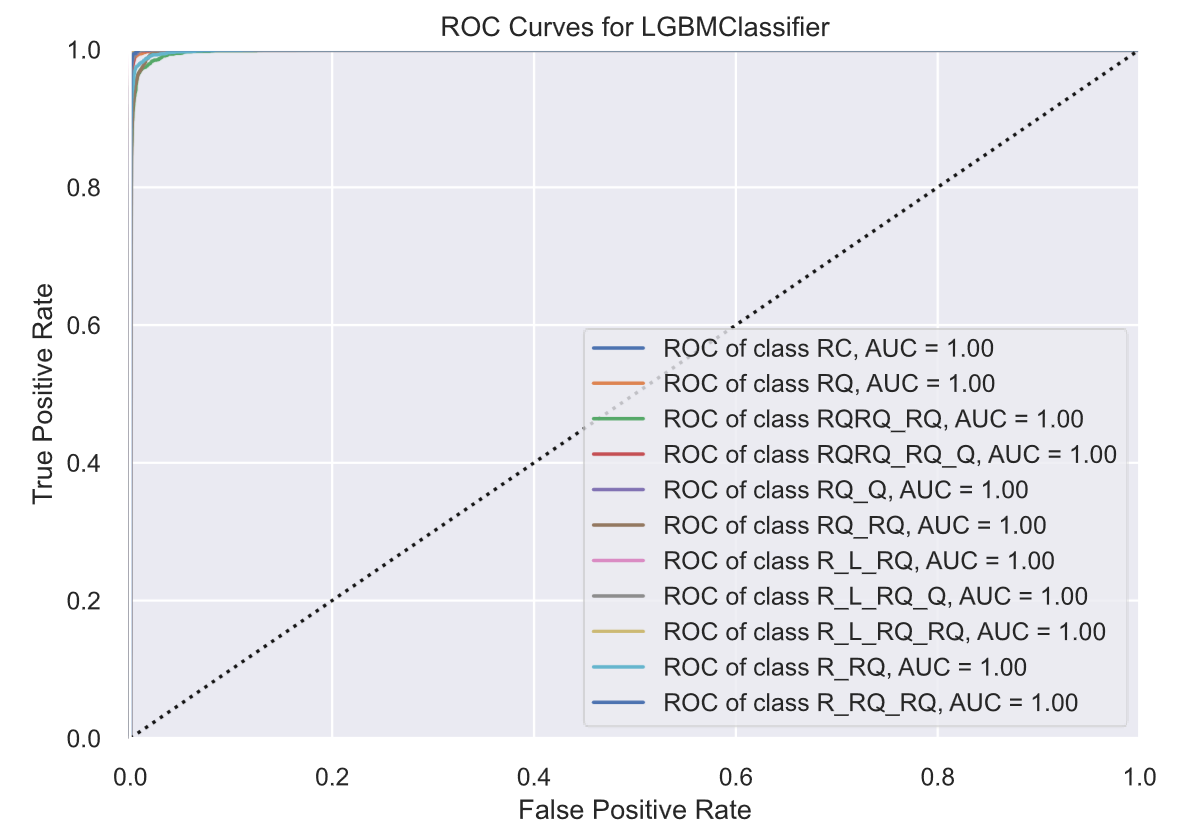
\includegraphics[width=0.9\textwidth]{Figuras/curva ROC por classe para o LGBM.png}
    \legend{Fonte: Imagem gerada pelo script de treinamento.}
    \label{figura38}
\end{figure}

A curva ROC do LGBM atingiu AUC=1.0 para todas as 11 classes, igualando o XGB e
superando o RF (que havia registrado AUC=0.99 para R\_RQ). O LGBM alcançou esse
resultado com tempo de treinamento cerca de 2.6 vezes menos que XGB (21 minutos vs. 56
minutos), como ilustrado na Figura~\ref{figura38}.

\begin{figure}[htbp]
    \centering
    \caption{Matriz de confusão do LGBM sobre o conjunto de teste. As confusões
    mais expressivas ocorreram entre RQRQ\_{RQ} e RQRQ\_{RQ\_Q} (62 amostras) e entre
    RQ\_{RQ} e RQRQ\_{RQ} (67 amostras). A classe R\_{RQ} apresentou 119 erros totais,
    o maior valor entre as classes para este modelo.}
    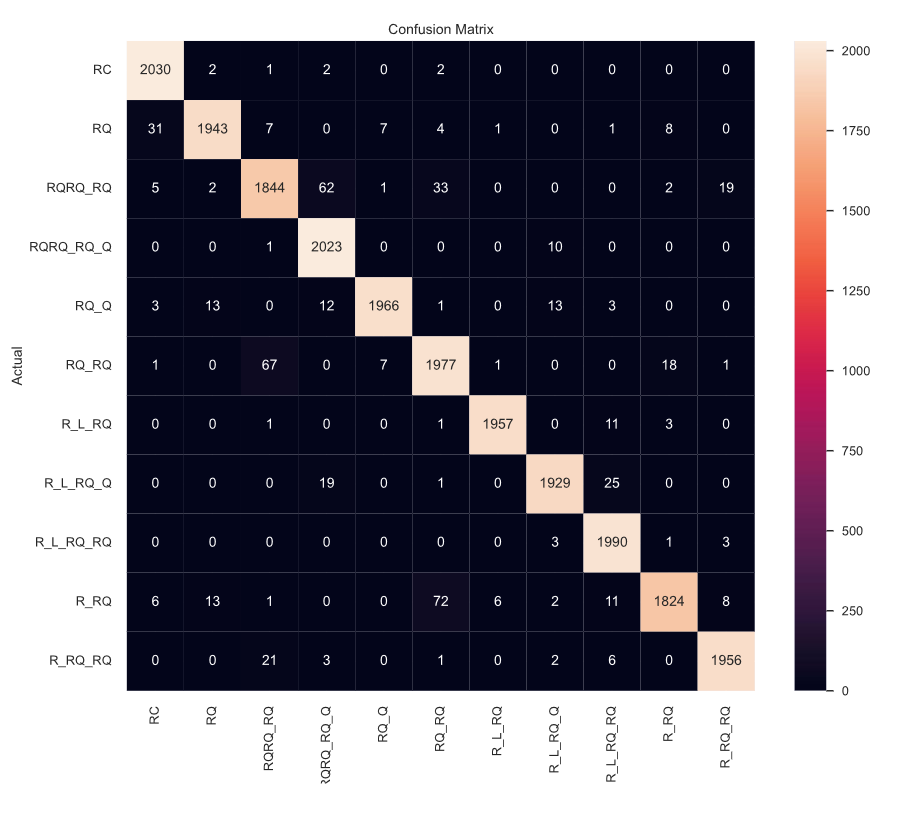
\includegraphics[width=0.9\textwidth]{Figuras/matriz de confusão do LGBM sobre o conjunto de teste.png}
    \legend{Fonte: Imagem gerada pelo script de treinamento.}
    \label{figura39}
\end{figure}

A matriz de confusão do LGBM é a mais limpa entre todos os modelos avaliados,
com menores valores absolutos de erro na maioria das classes. As principais confusões foram
entre RQRQ\_{RQ} e RQRQ\_{RQ\_Q} (62 erros), entre RQ\_{RQ} e RQRQ\_{RQ} (67 erros),
e entre R\_{RQ} e RQ\_{R} (72 erros), além de 6 erros entre R\_{RQ} e R\_{L\_RQ}.
Destaque positivo para a classe RC, que obteve apenas 7 erros totais (2030 acertos em
2037 amostras), como ilustrado na Figura~\ref{figura39}.

Os resultados demonstram claramente dois grupos distintos de desempenho. O primeiro grupo composto por LGBM, RF, XGB e Árvore de Decisão formado por modelos baseados em
árvores de decisão e alcançou acurácias de validação cruzada entre 95,85\% e 97,54\%,
superando amplamente a CNN (F1-score de 70,9\%). O segundo grupo formado pelos
modelos lineares (Regressão Logística, SVM, SGD e Naive Bayes) ficou restrito a
acurácias entre 9\% e 21\%, confirmando que os EIS não são linearmente separáveis. O LGBM
destacou-se como o melhor modelo geral, combinando a maior acurácia de validação cruzada
(97,54\%) com o menor tempo de treinamento entre os modelos de alto desempenho
($\sim$21 minutos). 

O RF apresentou resultado muito próximo (97,10\%) com uma estrutura
mais simples e interpretável. Ambos os modelos superam a CNN simultaneamente em
acurácia (97\% versus 71\%) e em eficiência computacional (21--34 minutos versus horas de
treinamento com 3 mil épocas), consolidando os métodos de ensemble baseados em árvores
como a abordagem mais adequada para este problema de classificação automática de
circuitos equivalentes.

\begin{figure}[htbp]
    \centering
    \caption{Relatório de classificação do LGBM. Os melhores resultados foram obtidos
    em $R\_{L\_RQ}$ (precisão 0,996; F1-score 0,994) e RC (recall 0,997; F1-score
    0,987). O menor F1-score foi registrado em RQRQ\_{RQ} (0,943), seguido de
    RQ\_{RQ} (0,950).}
    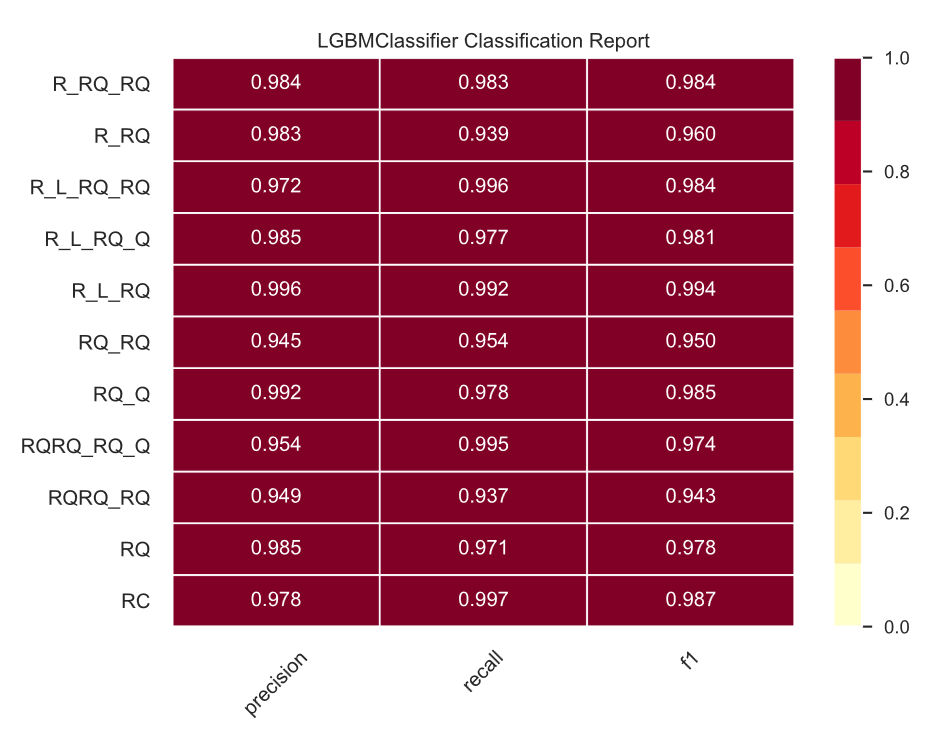
\includegraphics[width=0.9\textwidth]{Figuras/relatório de classificação LGDM.png}
    \legend{Fonte: Imagem gerada pelo script de treinamento.}
    \label{figura40}
\end{figure}

As melhores topologias são R\_L\_RQ atingiu os melhores resultados absolutos entre
todos os modelos e classes avaliados (precisão 0.996; recall 0.992; F1 0.994). TC também se
destacou com recall 0.997 e F1 0.987. R\_L\_RQ\_RQ (F1 0.984), R\_RQ\_RQ (F1 0.984) e
 R\_L\_RQ\_Q (F1 0.981) complementam o grupo das topologias mais bem identificadas. A piores
topologias são RQRQ\_RQ obteve o menor F1score entre as classes para LGBM (0.943), seguido de RQ\_RQ (0.950) – ambas classes que apresentam confusão reciproca elevada, como 
observado consistentemente em todos os modelos.

A análise conjunta dos resultados todos os modelos revelam um padrão consistente
quando às topologias mais ou menos identificáveis, independentemente do algoritmo utilizado.
R\_L\_RQ e RC aparece repetidamente como as classes mais bem classificadas, com F1-score
acima de 0.985 nos melhores modelos. Essas topologias possuem assinaturas espectrais mais
distintas: O circuito RC gera um arco semicircular característico no plano de Nyquist, enquanto
o R\_L\_RQ inclui o elemento indutivo L, que produz uma resposta de alta frequência exclusiva
e facilmente discriminável. R\_{L\_RQ\_RQ, R\_{RQ\_RQ} e R{QRQ\_RQ\_Q} também apresentaram
desempenho consistentemente alto, beneficiando-se da maior complexidade estrutural que gera
padrões espectrais mais únicos. R\_RQ foi a topologia mais difícil de classificar em todos os
modelos, com F1-score de 0.824 (KNN), 0.923 (Árvore de decisão), 0.943 (RF), 0.960 (XGB
e LGBM). Esse circuito é estruturalmente simples (um resistor em série) e seu espectro pode
ser facilmente confundindo com subconjuntos de topologias complexas que o contêm como
parte de sua estrutura. RQ\_RQ e RQRQ\_RQ também apresentaram desempenho abaixo da
média em todos os modelos, com confusões recíprocas frequentes entre si. Ambas as topologias
contêm dois elementos ZARC em série, diferindo apenas pela presença ou não de resistor
adicional, o que produz espectros com formas muito semelhantes em certas faixas de
frequência. Podendo ver na tabela~\ref{tab:3} e na Figura~\ref{figura41}.

\begin{table}[htb]
\caption{Comparativo geral dos modelos.}
\label{tab:3}
\centering
\begin{tabular}{lccc}
\toprule
\textbf{Modelo} & \textbf{Acurácia treino (\%)} & \textbf{Val. cruzada (\%)} & \textbf{Tempo de treino} \\
\midrule
LGBM            & 98,74 & 97,54 & $\sim$21 min \\
RF              & 99,54 & 97,10 & $\sim$34 min \\
XGB             & 98,15 & 96,81 & $\sim$56 min \\
Árvore decisão  & 99,54 & 95,85 & $\sim$9 min  \\
KNN             & 92,73 & 88,93 & $\sim$10 min \\
GB              & 86,29 & 85,34 & $\sim$37 h   \\
SGD             & 17,15 & 16,96 & $\sim$7 min  \\
Naïve Bayes     & 15,85 & 15,86 & $\sim$39 s   \\
SVM             & 20,91 & 17,64 & $\sim$5 h 54 min \\
RL              & 9,05  & 9,05  & $\sim$41 s   \\
\bottomrule
\end{tabular}
\legend{Fonte: Elaborado pelo autor.}
\end{table}

\begin{figure}[htbp]
    \centering
    \caption{Acurácia vs. Validação cruzada. Mostra claramente os dois grupos (alta/baixa performance) e a linha de referência da CNN.}
    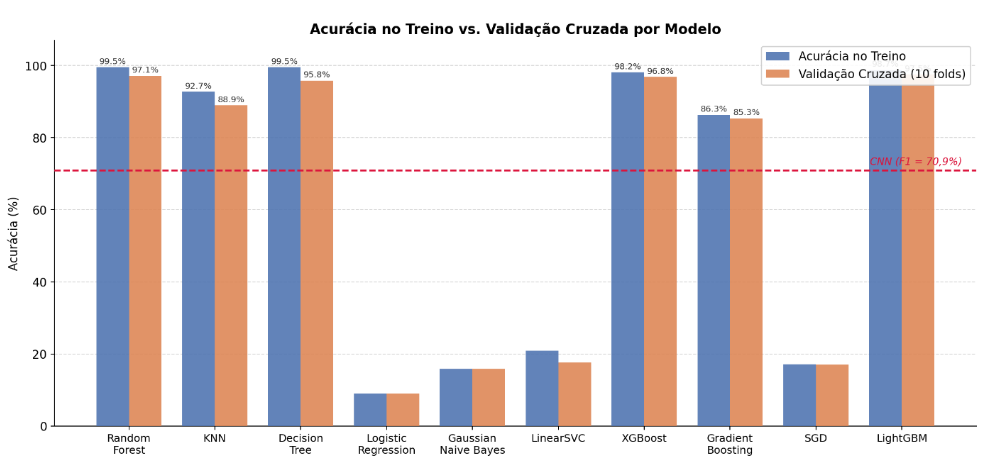
\includegraphics[width=0.9\textwidth]{Figuras/acurácia vs. Validação cruzada.png}
    \legend{Fonte: Imagem gerada pelo script de treinamento.}
    \label{figura41}
\end{figure}

Os resultados demonstram claramente dois grupos distintos de desempenho. O
primeiro grupo – composto por LGBM, RF, XGB e Árvore de decisão – são todos baseados em
árvores de decisão e alcançaram acurácias de validação cruzada entre 95.85\% e 97.54\%, superando amplamente a CNN (F1-score 70,9\%). O segundo grupo – formado pelos modelos
lineares (Regressão Logística, SVM, SGB e Naive Bayes) – ficou restrito a acurácia entre 9\%
e 21\%, confirmando que os EIS não são linearmente separáveis. O LGBM destacou-se como o
melhor modelo geral, combinando a maior acurácia de validação cruzada (97.54\%) com menor
tempo de treinamento entre os modelos de alto desempenho (~21 minutos). O RF apresentou
resultado muito próximo (97.10\%) com estrutura mais simples e interpretável. Ambos os
modelos superam a CNN simultaneamente em acurácia (97\% vs. 71\%) e em eficiência
computacional (21 – 34 minutos vs. Horas de treinamento com 3 mil épocas), consolidando os
métodos de ensemble baseados em árvores como a abordagem mais adequada para este
problema de classificação automática de circuitos equivalentes.

A análise do desempenho agregado, entretanto, não revela de forma completo o
comportamento dos modelos frente às diferentes topologias de circuito equivalente. Para
aprofundar essa avaliação. A Figura~\ref{figura42} apresenta o F1-score obtido por cada modelo para cada
uma das 11 topologias individualmente, permitindo identificar quais classes representam maior
desafio para os classificadores e em quais modelos convergem para resultados semelhantes.

\begin{figure}[htbp]
    \centering
    \caption{F1-score por topologia de circuito equivalente para os cinco melhores modelos avaliados (LBGM, RF, XGB, Árvore de decisão e KNN) e linha de referência da CNN (F1 médio $\approx$ 0.709). As regiões sombreadas em vermelho destacam as topologias RQ\_RQ, R\_RQ que apresentaram os menores F1-score de forma consistente entre todos os
    modelos.}
    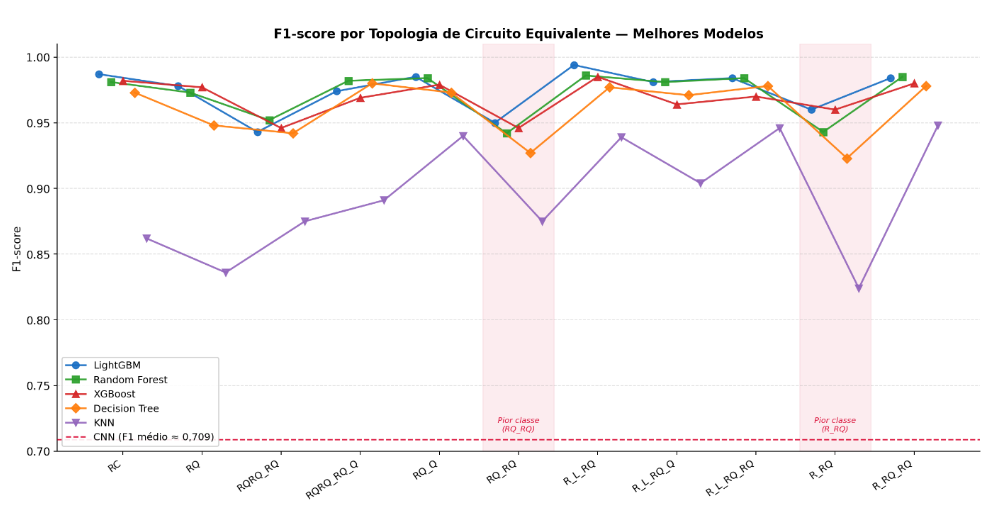
\includegraphics[width=0.9\textwidth]{Figuras/f1-score por topologia de circuito equivalente para os cinco melhores modelos avaliados.png}
    \legend{Fonte: Própria autoria.}
    \label{figura42}
\end{figure}

O gráfico confirma o padrão já discutido nas seções anterior: RC e R\_L\_RQ
como as topologias mais bem identificadas, e R\_RQ e RQ\_RQ como as mais desafiadoras e
evidencia que a superioridade dos modelos de ensemble sobre a CNN se mantém em todas as
11 topologias simultaneamente, e não apenas na média geral.

\chapter{CONCLUSÕES}
Este trabalho teve como objetivo desenvolver e avaliar modelos de aprendizado de
máquina capazes de identificar automaticamente o circuito equivalente associado a um espectro
de impedância eletroquímica (EIS), a partir de uma base de dados sintética composta por 110
mil espectros distribuídos entre onze topologia distintas. Para isso, foi construída uma
infraestrutura completa de geração, armazenamento e processamento dos dados, seguida da
avaliação sistemática de diferentes abordagens de classificação, desde redes neurais
convolucionais até algoritmos clássicos de aprendizado de máquina.

Os resultados obtidos evidenciaram diferenças expressivas de desempenho entre as
abordagens testadas. A rede neural convolucional (CNN), apesar de apresentar resultados
consistentes, alcançou F1-score de aproximadamente $70,9\%$, ficando atrás dos modelos
baseados em ensembles de árvores. Entre este, O LGBM destacou-se como o melhor modelo
geral, combinando a maior acurácia de validação cruzada $97,54\%$ ao menor tempo de
treinamento entre os modelos de alto desempenho, seguido de perto pelo RF $(97,10\%)$ e pelo
XGB $(96,81\%)$. Já os modelos lineares, como Regressão Logística, SVM e SGD, apresentaram
desempenho próximo ao acaso, confirmando que a relação entre os atributos espectrais e as
classes de circuito equivalente é fortemente não linear.

A análise detalhada dos erros mostrou um padrão consistente entre todos os
modelos avaliados: as topologias R\_RQ e RQ\_RQ, estruturalmente mais simples e semelhantes
a subconjuntos de outras topologias, concentraram a maior parte das confusões, enquanto RC e
R\_L\_RQ, com assinaturas espectrais mais distintas, foram consistentemente as mais bem
classificadas. Por esse motivo, já se encontra em andamento a etapa de continuidade deste
trabalho, na qual ruídos é deliberadamente adicionado aos espectros sintéticos de treinamento,
com o objetivo de aproximar as condições simuladas das características observadas em
medições reais de laboratório. Resultados preliminares dessa etapa, obtidos com diferentes
níveis de ruído $(1\%$ a $5\%)$ aplicados na mesma base de espectros. Já mostram o comportamento
esperado: O XGB manteve-se como o modelo mais robusto nesse cenário mais realista, com
acurácia de $72,46\%$ no conjunto de teste, e a taxa de erro cresceu de forma consistente com o
aumento do nível de ruído, passando de $4,8\%$ para espectros sem ruído a $32,1\%$ para o maior
nível avaliado. Esses resultados confirmam a relevância dessa etapa para uma avaliação mais
fiel da aplicabilidade dos modelos em condições experimentais reais.

Como trabalho futuros,
pretende-se dar continuidade ao aprimoramento dos modelos de classificação, com ajuste de
hiperparâmetros e novas estratégias de pré-processamento, buscando um modelo que alie robustez ao ruído experimental e desempenho suficiente para viabilizar a automatização do
processo de identificação de circuitos equivalentes no laboratório. Pretende-se, ainda, ampliar
o escopo da automação para além da etapa de classificação, explorando o uso de modelos de
aprendizado de máquina também no ajuste de curva (curve fitting) dos parâmetros do circuitos
equivalentes, de modo a cobrir todo o fluxo de análise de dados de espectroscopia de
impedância eletroquímica.
\pagebreak




% ----------------------------------------------------------
% ELEMENTOS PÓS-TEXTUAIS
% ----------------------------------------------------------
%!TEX root = ./main.tex
%%%%%%%%%%%%%%%%%%%%%%%%%%%%%%%%%%%%%%%%%%%%%%%%%%%%%%%%%%%%%%%%%%%%%%%%%%%%%%%%%%
% ----------------------------------------------------------
% ELEMENTOS PÓS-TEXTUAIS
% ----------------------------------------------------------
\postextual
% ----------------------------------------------------------

% ----------------------------------------------------------
% Referências bibliográficas
% ----------------------------------------------------------
\bibliography{bibliografia}

% ----------------------------------------------------------
% Glossário
% ----------------------------------------------------------
%
% Consulte o manual da classe abntex2 para orientações sobre o glossário.
%
%\glossary

% ----------------------------------------------------------
% Apêndices
% ----------------------------------------------------------

% ---
% Inicia os apêndices
% ---

% ---


% ----------------------------------------------------------
% Anexos
% ----------------------------------------------------------

% ---
% Inicia os anexos
% ---


%---------------------------------------------------------------------
% INDICE REMISSIVO
%---------------------------------------------------------------------
\phantompart
\printindex
%---------------------------------------------------------------------


\end{document}

%%%%%%%%%%%%%%%%%%%%%%%%%%%%%%%%%%%%%%%%%%%%%%%%%%%%%%%%%%%%
%%%%%%%%%%%%%%%%%%%%%%%%%%%%%%%%%%%%%%%%%%%%%%%%%%%%%%%%%%%%
%% Links de algumas NBRs:

% -------------------------------------------
% ABNT NBR 14724:2011 - Trabalhos acadêmicos 
% -------------------------------------------
% http://site.ufvjm.edu.br/revistamultidisciplinar/files/2011/09/NBR_14724_atualizada_abr_2011.pdf

% -----------------------------
% ABNT NBR 6027:2012 - Sumário
% -----------------------------
% https://cnm.paginas.ufsc.br/files/2020/02/ABNT-NBR-6027.pdf

% ---------------------------------
% ABNT NBR 6023:2018 - Referências
% ---------------------------------
% https://www.ufpe.br/documents/40070/1837975/ABNT+NBR+6023+2018+%281%29.pdf/3021f721-5be8-4e6d-951b-fa354dc490ed

% ----------------------------------------------------------------------
% ABNT NBR 6024:2012 - Numeração progressiva das seções de um documento
% ----------------------------------------------------------------------
% https://cnm.paginas.ufsc.br/files/2020/02/ABNT-NBR-6024.pdf

% ------------------------------------------------
% ABNT NBR 6028:2021 - Resumo, resenha e recensão
% ------------------------------------------------
% http://plone.ufpb.br/secretariado/contents/documentos/2021_ABNT6028Resumo.pdf

% ----------------------------
% ABNT NBR 6034:2004 - Índice
% ----------------------------
% https://cnm.paginas.ufsc.br/files/2020/02/ABNT-NBR-6034.pdf

% --------------------------------------------
% ABNT NBR 10520:2023 - Citações em documentos
% --------------------------------------------
% http://www.cbiotec.ufpb.br/secretariado/contents/documentos/abnt-docs/2023_abnt-10520-citacoes.pdf

% ----------------------------------------------------------
%%%% Falta: ABNT NBR 12225: 2023 - Lombada
%% Não consegui encontrar o PDF disponível online. Uma descrição do que mudou em relação à versão passada:
%% https://www.infonormas.com.br/2023/05/16/saiu-nova-norma-abnt-que-pode-ser-aplicada-ao-seu-trabalho-academico-tcc-2023/
% ----------------------------------------------------------

%%%%%%%%%%%%%%%%%%%%%%%%%%%%%%%%%%%%%%%%%%%%%%%%%%%%%%%%%%%%%%%%%%%%%%%%%%%%%%%%%%%%%%%%%%%%%%%%%%%%%%%%%%
%%% ATENÇÃO: antes de se basear nas normas, verifique se a versão é a atual.
%%%
%%% Algumas Universidades ou cursos possuem regras extras e/ou formatação específica 
%%% Ex: a UFSM possui normas MDT (Manual de Dissertações e Teses) para elaboração de trabalhos acadêmicos.
%%%%%%%%%%%%%%%%%%%%%%%%%%%%%%%%%%%%%%%%%%%%%%%%%%%%%%%%%%%%%%%%%%%%%%%%%%%%%%%%%%%%%%%%%%%%%%%%%%%%%%%%%%

%% EOF